\documentclass[11pt]{article}
\usepackage[UTF8]{ctex}
\usepackage[preprint]{acl}
\usepackage{times}
\usepackage{latexsym}
\usepackage{graphicx}
\usepackage{booktabs}
\usepackage{multirow}
\usepackage{amsmath}
\usepackage{amssymb}
\usepackage{amsthm}
\usepackage{mathtools}
\usepackage{enumitem}
\usepackage{tikz}
\usetikzlibrary{arrows.meta,positioning,shapes.geometric,fit,backgrounds}

\setcounter{topnumber}{4}
\setcounter{bottomnumber}{4}
\setcounter{totalnumber}{8}
\setcounter{dbltopnumber}{4}
\renewcommand{\topfraction}{0.95}
\renewcommand{\bottomfraction}{0.95}
\renewcommand{\textfraction}{0.05}
\renewcommand{\floatpagefraction}{0.85}
\renewcommand{\dbltopfraction}{0.95}
\renewcommand{\dblfloatpagefraction}{0.85}

\newtheorem{theorem}{定理}
\newtheorem{proposition}{命题}
\newtheorem{lemma}{引理}
\newtheorem{definition}{定义}

\title{\textbf{U-GraphRAG}：基于不确定性路由、冲突感知证据选择与校准解码的可靠检索增强生成}

\author{
  \textbf{周兴} \quad \textbf{宋丽} \\
  计算机与人工智能学院 \\
  山东财经大学 \\
  \texttt{zhouxing@sdufe.edu.cn}, \texttt{LindaSong@gmail.com}
}

\begin{document}
\maketitle

\begin{abstract}
在充满噪声、多跳关联与潜在事实冲突的语料库上部署检索增强生成（RAG）系统时，现有方法面临三类相互耦合的技术瓶颈：（1）固定 Top-$K$ 检索在简单查询上耗费 $50\%\text{--}80\%$ 的冗余上下文 Token，而未经跨模型标定的熵阈值在同质无关候选池（Scenario S4）上容易引发无效早退；（2）最大边际相关性（MMR）等表面多样性方法缺乏事实冲突辨别力（保留 $>95\%$ 的注入矛盾文档），而直接施加无条件概率散度惩罚又会过度抑制分别承载不同推理跳数的互补桥接文档；（3）对比解码虽可通过扣除无上下文先验增强事实依从性，但直接依据对比缩放与截断后的 Logits 估计置信度会导致严重的过度自信偏移，推高期望校准误差（ECE）。

本文提出一种免训练、适配单卡显存约束的可靠 RAG 框架 \textbf{U-GraphRAG}，包含三个协同阶段：\textbf{M1} 利用首词元预测熵估计认知不确定性，结合开发集分位数标定以及查询相关性与词面重叠双重安全门控控制检索早退，并在需要扩展时通过布隆过滤器与 MinHash LSH 哈希图筛出高关联候选文档；\textbf{M2} 基于词面重叠触发的 Jensen-Shannon 散度惩罚筛选基数受限的证据子集，并利用 Kruskal 最大生成森林与根优先深度优先遍历排序输出上下文；\textbf{M3} 将 $\beta=0.12$ 对比生成轨迹与 $\beta=0$ 无调节上下文概率采集分离，再联合单调 Platt 校准与有限样本划分共形预测（Split Conformal Prediction）完成选择性拒答控制。在涵盖 \textbf{324 组多种子主实验}（$71,280$ 次评估）、\textbf{6 维 22 档受控压力测试}（$7,920$ 次评估）、\textbf{跨域零调优迁移}（$2,080$ 次评估）以及与 \texttt{BGE-Reranker-Large}、\texttt{CK-PLUG}（ICLR'26）、\texttt{InstructRAG-ICL}（ICLR'25）和 \texttt{CAD}（NAACL'24）同口径对照的 \textbf{15,960 次评测}——累计 \textbf{97,240 次测试推理}上：U-GraphRAG 取得 12 区块最高的宏平均 F1（\textbf{52.05\%}，Friedman $p = 1.37 \times 10^{-10}$），将宏平均 ECE 降低 \textbf{78.8\%}（\textbf{0.0720} vs.\ 0.3404，Friedman $p = 9.90 \times 10^{-6}$）；在公开反事实基准 \texttt{NQ-Swap Dual} 上于三个基座模型上均位居首位（较最强基线高 \textbf{+7.32 至 +28.56 pp}），在混合冲突基准 \texttt{RAMDocs} 的 \texttt{Qwen2.5-7B} 模型上取得 \textbf{69.40\% Raw F1 / 75.58\% 选择性精度}，将 \texttt{HotpotQA} 冲突文档保留率由 \textbf{72.5\%--100\% 降至 9.17\%--10.00\%}，并在全无关检索池 S4 上消除了最高 \textbf{85.83 pp} 的无效早退（门控后 \textbf{0.0\%} 漏放行且实现 100\% 安全拒答）。
\end{abstract}

\section{引言 (Introduction)}

检索增强生成（RAG）通过引入外部非参数化知识库，有效缓解了大语言模型（LLM）的参数知识陈旧性与幻觉问题 \cite{yang2018hotpotqa,mallen2023popqa}。尽管近年来顶会文献在冲突消解 RAG \cite{wei2025instructrag,xiang2024robustrag,wang2025madamrag,bi2026ckplug}、不确定性自适应检索 \cite{su2024dragin,jeong2024adaptiverag,yao2025seakr,adarague2025} 以及对比解码与共形校准 \cite{shi2024cad,gema2025decore,sinha2025crg} 三条赛道上取得了重要进展，但在严格的单卡显存与低延迟约束下构建高可靠 RAG 系统，仍存在三个亟待解决的方法学矛盾：

\begin{enumerate}[leftmargin=*,nosep]
    \item \textbf{跨模型家族熵尺度差异与无效早退风险（M1 层面）}：不同架构 LLM 的首词元预测熵具有明显不同的数值尺度（例如在 \texttt{HotpotQA} 开发集上，\texttt{Qwen2.5-3B}、\texttt{Qwen2.5-7B} 与 \texttt{Llama-3.1-8B} 的第 60 分位认知不确定性估计值分别为 $0.2015$、$0.0749$ 与 $0.6281$）。固定标量阈值难以直接跨模型通用；此外，当初始检索集 $\mathcal{D}_0$ 全为表层相近但偏离查询主题的无关文档（Scenario S4），或潜伏未触发警戒的高分矛盾文档时，模型熵值仍可能保持在较低水平，从而引发无效早退。
    \item \textbf{互补多跳桥接保留与矛盾文档清除的两难问题（M2 层面）}：在多跳推理中，首跳桥接文档 $d_1$（如指明影片导演姓名）与次跳答案文档 $d_2$（如给出该导演的出生地）各自单独提供时，诱导出的下一词元预测分布天然存在显著差异（$D_{\text{JS}}(P_1 \parallel P_2) \gg 0$）。若直接施加无门控的 JS 散度惩罚，当冲突权重 $\lambda_4$ 从 $1.0$ 增至 $10.0$ 时，\texttt{HotpotQA} 干净测试集的支持事实召回率从 $90.62\%$ 下降至 $56.25\%$，F1 从 $46.63\%$ 降至 $22.64\%$；相反，基于表面多样性的 MMR \cite{carbonell1998mmr} 无法区分事实矛盾，会保留高达 $96.25\%$ 的注入冲突文档。
    \item \textbf{对比解码增强与概率校准失真之间的内在冲突（M3 层面）}：CAD \cite{shi2024cad} 与 CK-PLUG \cite{bi2026ckplug} 等方法通过 $(1+\beta)\mathbf{z}_t^{\text{ctx}} - \beta\mathbf{z}_t^{\text{prior}}$ 放大上下文依赖信号，但我们从理论上证明并经消融实验证实：直接在对比调节与尾部截断后的 Logits 上计算生成概率，会剔除尾部概率质量并推高最大词元概率，破坏置信度排序能力（\texttt{HotpotQA} 判别 AUROC 仅 $0.5267$，错误拒答率达 $43.75\%$）。
\end{enumerate}

本文在单卡 RTX 4090（4-bit NF4 量化）预算下系统构建了可校准选择性 RAG 框架 \textbf{U-GraphRAG}，全面报告其核心技术原理与理论证明、多种子跨家族主基准评测、6 维单变量受控压力测试、零调优跨域迁移、划分共形风险控制审计，以及与 \texttt{BGE-Reranker}、\texttt{CK-PLUG}、\texttt{InstructRAG-ICL} 及 \texttt{CAD} 等近期免训练强基线的同口径对比分析。

\section{相关工作与顶会基线循证定位 (Related Work)}

基于对 2024--2026 年顶会文献的循证梳理，相关工作可分为三大赛道：

\paragraph{赛道 A：冲突消解与鲁棒 RAG。}
\textbf{InstructRAG} \cite{wei2025instructrag} 通过自合成去噪推理链（Rationale）显式引导模型过滤噪声，但其最强微调版（FT）需针对各数据集单独多卡微调。 \textbf{RobustRAG} \cite{xiang2024robustrag} 采用“隔离生成再安全聚合（Isolate-then-Aggregate）”架构提供可证明抗篡改鲁棒性，但带来 $1.16\text{--}3.65$ 倍延迟且在错误源占多数时投票易受冲击。 \textbf{MADAM-RAG} \cite{wang2025madamrag} 为每篇文档分配独立 Agent 进行多轮辩论，在 AmbigDocs 上领先 Astute RAG $11.40\%\text{--}12.90\%$，但在高强度混合冲突集 RAMDocs 上 EM 仍仅 $34.40\%$，且在 \texttt{Qwen2.5-7B} 上显存占用高达 $29.44\text{ GB}$（超出单张 RTX 4090 的 $24\text{ GB}$ 上限）。 \textbf{CK-PLUG} \cite{bi2026ckplug} 利用参数与上下文预测的置信增益（Confidence Gain）实现免训练 Token 级冲突调控，但未对调制后的概率分布进行下游校准或选择性拒答控制。此外，\textbf{Astute RAG} \cite{wang2025astuterag}、\textbf{Knowledgeable-R1} \cite{knowledgeabler1_2026} 与 \textbf{ReliabilityRAG} \cite{reliabilityrag2025} 分别探索了内外知识对齐、GRPO 强化学习与 NLI 最大独立集采样。

\paragraph{赛道 B：不确定性驱动与自感知自适应检索。}
\textbf{DRAGIN} \cite{su2024dragin} 与 \textbf{Adaptive-RAG} \cite{jeong2024adaptiverag} 分别基于生成期实时 Token 熵或预训练复杂度分类器动态触发检索；\textbf{SEAKR} \cite{yao2025seakr} 与 \textbf{Internal Confidence} \cite{chen2026internalconfidence} 提取 LLM 内部隐层 Gram 行列式或决策中心层表征评估知识边界；\textbf{Self-RAG} \cite{asai2024selfrag} 与 \textbf{CRAG} \cite{yan2024crag} 则引入反思微调或外部 $0.77\text{B}$ 评估器。尤为关键的是，ACL 2025 综述基准 \textbf{AdaRAGUE} \cite{adarague2025} 在 6 大数据集上同口径复现了 Adaptive-RAG、DRAGIN、FLARE 与 SEAKR，实证表明轻量级不确定性指标在检索路由决策上的表现与复杂的隐层自感知探针相当——这为 U-GraphRAG M1 采用基于单次前向熵的解析估计算子提供了循证支撑，同时凸显了在全无关候选池（Scenario S4）上增设相关性下界门控的必要性。

\paragraph{赛道 C：对比解码、校准与共形风险控制。}
\textbf{CAD} \cite{shi2024cad}、\textbf{DoLa} \cite{chuang2024dola} 与 \textbf{DeCoRe} \cite{gema2025decore} 通过上下文或检索头对比解码降低幻觉。在风险校准方面，\textbf{CRG} \cite{sinha2025crg} 揭示了著名的“语义幻觉（Semantic Illusion）”负结果：在合成集上达到 $0.81\text{--}0.83$ AUROC 和 $0\%$ 误报率的检测器，在真实 HaluEval 的 $95\%$ 召回约束下误报率退化至 $100\%$（跨分布 $\text{NQ}\to\text{RAGTruth}$ 覆盖率从 $95\%$ 跌至 $11\%$）。近期 \textbf{CoFact} \cite{cofact2026} 与 \textbf{DualStake} \cite{dualstake2026} 进一步探索了共形事实覆盖与选择性预测 AURC 优化。U-GraphRAG 在单卡免训练架构中有机整合了 M1 安全路由检索、M2 重叠门控证据优选排序，以及 M3 无调节概率校准与有限样本共形风险控制。

\section{方法论：基础预备知识、核心原理与系统架构 (Methodology)}

为确保方法推导的自洽性与可读性，我们在形式化 M1--M3 模块之前，依次阐明本框架所依托的基础网络架构、信息检索原语、哈希索引结构、信息论度量、图论遍历及统计校准方法的提出背景、基本思想与具体用途。

\subsection{基础预备知识与总体架构}
\label{sec:zh_prelim}

\paragraph{自回归 Transformer 语言模型与 4-bit NF4 量化。}
本文所采用的大语言模型均基于 \citet{vaswani2017attention} 提出的 \textbf{Transformer 架构}。与按时间步串行递推的循环神经网络不同，Transformer 通过并行化的多头缩放点积自注意力（Multi-Head Scaled Dot-Product Self-Attention）机制直接建模任意位置词元间的长程语义关联，并配合位置前馈网络与残差归一化层实现深层表征。在因果语言建模中，下三角因果注意力掩码确保第 $t$ 步的预测分布 $P_{\theta}(y_t \mid q, \mathcal{E}, y_{<t}) = \mathrm{Softmax}(\mathbf{z}_t)$ 仅依赖输入查询 $q$、检索证据 $\mathcal{E}$ 与已生成前缀 $y_{<t}$。为在不更新模型参数的条件下将 3B--8B 模型权重容纳至单张消费级 GPU（$<24\text{ GB}$ 显存），我们采用 \citet{dettmers2023qlora} 提出的 \textbf{4-bit NormalFloat（NF4）量化}技术：针对神经网络权重近似正态分布的统计特性，按标准正态分布等概率分位数划定 4-bit 量化桶，在基本保持冻结模型前向输出一致性的前提下将显存需求压缩至约四分之一。

\paragraph{稀疏、稠密与秩融合一阶段检索原语。}
给定自然语言查询 $q \in \mathcal{Q}$ 与外部语料库 $\mathcal{C} = \{d_1, \dots, d_M\}$，一阶段检索器结合词面精确匹配与稠密语义表征获取初始候选：
\begin{itemize}[leftmargin=*,nosep]
    \item \textbf{BM25 稀疏检索模型} \cite{robertson2009bm25}：由 Robertson 与 Zaragoza 系统提出，基于概率相关性框架对逆文档频率（IDF）、词频饱和效应与文档长度归一化进行建模，对人名、地名与专有实体具有稳定的精确匹配能力。
    \item \textbf{稠密双编码器检索} \cite{karpukhin2020dpr}：由 Karpukhin 等人在开放域问答中系统验证，利用神经网络将查询与段落分别映射至同一低维向量空间（本文采用 \texttt{BAAI/bge-small-en-v1.5}~\cite{chen2024bgem3}），通过向量内积捕捉缺乏共同关键词的同义改写关联。
    \item \textbf{倒数秩融合（RRF）} \cite{cormack2009rrf}：由 Cormack 等人提出，针对稀疏检索分与向量相似度尺度不可直接相加的问题，仅依据各自排序名次计算融合得分 $\text{RRF}(d) = \sum_r (k + \text{rank}_r(d))^{-1}$（本文固定 $k=60$）。由此得到初始种子集 $\mathcal{D}_0 = (d_1, \dots, d_{k_0})$（$k_0 = 3$）及候选池 $\mathcal{D}_{\text{pool}}$（$|\mathcal{D}_{\text{pool}}| \le 16$）。
    \item \textbf{最大边际相关性（MMR）} \cite{carbonell1998mmr}：由 Carbonell 与 Goldstein 提出的多样性重排经典算法，在迭代选择文档时权衡查询相关性与已选文档的表面相似度。尽管 MMR 能有效削减词汇重复，但无法辨别“高重叠且事实矛盾”的伪证片段，这正是后续模块 M2 需要重点解决的缺陷。
\end{itemize}

\begin{figure*}[t]
\centering
\resizebox{\textwidth}{!}{
\begin{tikzpicture}[
    node distance=0.55cm and 0.85cm,
    box/.style={rectangle, rounded corners=4pt, draw=black!70, thick, align=center, font=\small, inner sep=6pt, fill=white},
    m1box/.style={box, fill=blue!6, draw=blue!65!black},
    m2box/.style={box, fill=teal!6, draw=teal!65!black},
    m3box/.style={box, fill=orange!7, draw=orange!70!black},
    gatebox/.style={box, fill=red!6, draw=red!65!black},
    arr/.style={-{Latex[length=2.4mm]}, thick, draw=black!80},
    dasharr/.style={-{Latex[length=2.4mm]}, thick, dashed, draw=green!50!black}
]
% Stage 0
\node[box, fill=gray!8] (inp) {\textbf{查询与混合检索池}\\查询 $q$, $\text{RRF}_{k=60}$ 排序\\初始种子 $\mathcal{D}_0$ ($k_0=3$)\\候选池 $\mathcal{D}_{\text{pool}}$ ($|\mathcal{D}|\le 16$)};

% Stage 1: Module M1
\node[m1box, right=0.75cm of inp] (m1p) {\textbf{M1 首词元熵估计}\\单次 Top-$V_k$ ($V_k=48$)\\$H_{\text{total}} \to U_{\text{AU}}, U_{\text{EU}}$\\开发集分位数 $\tau_{\text{EU}}^{(m)}$};
\node[gatebox, below=0.48cm of m1p] (m1g) {\textbf{M1 安全路由门控}\\相关性下界 $\mathcal{G}_{\text{rel}}(q, \mathcal{D}_0)$\\冲突重叠 $\mathbb{I}_{\text{conflict}}$ ($J_3\ge 0.20$)\\决策：$\text{EE} \in \{0,1\}$};
\node[m1box, right=0.80cm of m1p] (m1e) {\textbf{M1 布隆与图扩展}\\双哈希布隆剪枝（零漏报）\\64 置换 MinHash LSH\\碰撞图 $G_{\text{LSH}} \to \mathcal{D}_{\text{cand}}$};

% Stage 2: Module M2
\node[m2box, right=0.80cm of m1e] (m2g) {\textbf{M2 重叠冲突门控}\\指数调节可靠度 $\tilde{R}_i$\\3-shingle 门控 $\mathbb{I}[R_{ij}\ge 0.20]$\\散度惩罚 $K_{ij}^{\text{gated}}(D_{\text{JS}}, C_{ij})$};
\node[m2box, below=0.48cm of m2g] (m2o) {\textbf{M2-A/B 证据优选}\\基数受限精确子集 ($k\le 5$)\\Kruskal 最大生成森林\\根优先 DFS $\pi(\mathcal{D}^*)$};

% Stage 3: Module M3
\node[m3box, right=0.85cm of m2g] (m3d) {\textbf{M3 对比答案生成}\\对比 Logits ($\beta=0.12$)\\$\alpha_{\text{tr}}=0.10$, 终止符保护\\输出答案轨迹 $\hat{\mathbf{y}}$};
\node[m3box, below=0.48cm of m3d] (m3c) {\textbf{M3 Platt 与共形控制}\\无调节 $\beta=0$ 原始概率 $/ T$\\Platt $(a^*, b^*) + r_{\text{ev}} + \text{SynChk}$\\Split 共形阈值 $\hat{\tau}_{\text{conf}}^{\text{SC}}(\alpha) \to \hat{c}$};

% Output
\node[box, fill=gray!8, right=0.75cm of m3d, yshift=-0.95cm] (out) {\textbf{高可靠输出元组}\\$(\hat{\mathbf{y}}, \hat{c}, \text{Abstain})$\\触发安全拒答若\\$\hat{c} < \hat{\tau}_{\text{conf}}^{\text{SC}}$ 或 $\neg \mathcal{G}_{\text{rel}}$};

% Edges
\draw[arr] (inp) -- (m1p);
\draw[arr] (m1p) -- (m1g);
\draw[arr] (m1g.east) -| node[pos=0.25, above, font=\scriptsize] {$\text{EE}=0$} (m1e.south);
\draw[arr] (m1e) -- (m2g);
\draw[arr] (m2g) -- (m2o);
\draw[arr] (m2o.east) -- ++(0.32,0) |- (m3d.west);
\draw[arr] (m3d) -- (m3c);
\draw[arr] (m3d.east) -| (out.north);
\draw[arr] (m3c.east) -| (out.south);

% Fast Path Early Exit
\draw[dasharr] (m1g.south) -- ++(0,-0.55) -| node[pos=0.22, below, font=\scriptsize\bfseries, text=green!45!black] {安全早退捷径 ($\text{EE}=1$)：跳过 M1 图扩展与 M2（$\mathcal{D}^*=\mathcal{D}_0$，至高节省 84\% Token）} (m2o.south);
\end{tikzpicture}
}
\caption{\textbf{U-GraphRAG} 整体系统架构图。模块 M1 在相关性下界与重叠冲突双重安全门控（$\mathcal{G}_{\text{rel}}$ 与 $\mathbb{I}_{\text{conflict}}$）约束下估计首词元认知不确定性并控制检索早退；当 $\text{EE}=0$ 时经布隆过滤与 MinHash LSH 扩展候选图送入 M2，通过重叠门控 JS 惩罚与 Kruskal 最大生成森林净化并重排证据；M3 将 $\beta=0.12$ 对比生成轨迹与 $\beta=0$ 无调节概率采集分离，联合 Platt 缩放与划分共形预测实现风险受控的选择性输出。}
\label{fig:zh_arch}
\end{figure*}

在冻结的 4-bit NF4 因果 Transformer 语言模型 $P_{\theta}(y \mid q, \mathcal{E})$ 下，U-GraphRAG 通过图~\ref{fig:zh_arch} 所示的三阶段流水线输出带有校准置信度与拒答标识的三元组 $(\hat{\mathbf{y}}, \hat{c}, \text{Abstain}) \in \mathcal{V}^* \times [0, 1] \times \{0, 1\}$。

\subsection{模块 M1：不确定性路由的自适应检索与候选图扩展}

\subsubsection{首词元香农熵估计与不确定性分解}
\paragraph{基础方法：香农熵与偶然/认知不确定性二分。}
\citet{shannon1948mathematical} 在信息论中提出\textbf{香农熵（Shannon Entropy）}$H(P) = -\sum_v p(v)\ln p(v)$，用于刻画离散随机变量概率分布的不确定性或平均信息量：分布越平缓均匀则熵越高，概率高度集中于单一取值则熵趋于零。在机器学习不确定性量化领域，\citet{hullermeier2021aleatoric} 系统阐述了预测总不确定性的双重来源：\textbf{偶然不确定性（Aleatoric Uncertainty）}源自输入表达或局部语境本身固有的歧义性与不可约噪声；而\textbf{认知不确定性（Epistemic Uncertainty）}源自模型当前所获知识或外部证据不足，可通过补充检索或消解冲突予以降低。为避免多次随机前向采样带来的高额单卡延迟，M1 仅执行一次非自回归前向计算（\texttt{use\_cache=False, logits\_to\_keep=1}），截取首答案词元在 Top-$V_k$（$V_k = 48$）词表支撑集 $\mathcal{V}_k \subset \mathcal{V}$ 上的分布，并计算归一化香农预测熵：
\begin{align}
H_{\text{total}}(q, \mathcal{D}_0) &= -\sum_{v \in \mathcal{V}_k} \tilde{p}(v \mid q, \mathcal{D}_0) \nonumber \\
&\qquad \cdot \ln \tilde{p}(v \mid q, \mathcal{D}_0), \label{eq:zh_m1_htotal} \\
\tilde{p}(v \mid q, \mathcal{D}_0) &= \frac{P_{\theta}(v \mid q, \mathcal{D}_0)}{\sum_{w \in \mathcal{V}_k} P_{\theta}(w \mid q, \mathcal{D}_0)}. \nonumber
\end{align}
设 $\mathcal{W}(d_i)$ 为文档 $d_i \in \mathcal{D}_0$ 的归一化词集合，通过种子文档间的平均成对 Jaccard 相似度 $\bar{J}(\mathcal{D}_0)$ 与词面分歧度 $D_{\text{lex}}(\mathcal{D}_0) = 1 - \bar{J}(\mathcal{D}_0)$ 反映检索上下文内部的表层分散程度：
\begin{equation}
\bar{J}(\mathcal{D}_0) = \frac{2}{|\mathcal{D}_0|(|\mathcal{D}_0|-1)} \sum_{i < j} \frac{|\mathcal{W}(d_i) \cap \mathcal{W}(d_j)|}{|\mathcal{W}(d_i) \cup \mathcal{W}(d_j)|}.
\label{eq:zh_m1_jbar}
\end{equation}
据此，偶然歧义分量 $U_{\text{AU}}$ 与认知路由信号 $U_{\text{EU}}$ 的解析分解定义为：
\begin{align}
U_{\text{AU}}(q, \mathcal{D}_0) &\triangleq \alpha_{\text{au}}\bigl(0.25 + 0.50 \, D_{\text{lex}}(\mathcal{D}_0)\bigr) \nonumber \\
&\quad \cdot H_{\text{total}}(q, \mathcal{D}_0), \label{eq:zh_m1_uau} \\
U_{\text{EU}}(q, \mathcal{D}_0) &\triangleq \max\bigl(0, \; H_{\text{total}} - U_{\text{AU}}\bigr). \label{eq:zh_m1_ueu}
\end{align}
在默认 $\alpha_{\text{au}} = 1.0$ 下，式~\eqref{eq:zh_m1_ueu} 简化为 $U_{\text{EU}}(q, \mathcal{D}_0) = (0.25 + 0.50 \, \bar{J}(\mathcal{D}_0)) H_{\text{total}}(q, \mathcal{D}_0) \ge 0$。对任意待扩展文档 $d_c \in \mathcal{D}_{\text{pool}} \setminus \mathcal{D}_0$，加入该文档所带来的边际认知不确定性消减量为 $\Delta U_{\text{EU}}(d_c \mid q, \mathcal{D}_0) = \max(0, U_{\text{EU}}(q, \mathcal{D}_0) - U_{\text{EU}}(q, \mathcal{D}_0 \cup \{d_c\})) \ge 0$。

\subsubsection{跨模型开发集分位数定标与双安全路由门控}
由于不同模型家族的词表概率锐度不同，我们仅在一个固定参考开发集 $\mathcal{D}_{\text{anchor}}^{\text{dev}}$（\texttt{HotpotQA} Dev, $N_{\text{dev}} = 80$）上按 $q_{\text{target}} = 0.60$ 分位数为每个基座单独标定阈值 $\tau_{\text{EU}}^{(m)}$，完全禁止针对测试集调参：
\begin{align}
\tau_{\text{EU}}^{(m)} &\triangleq \text{Clip}_{[0.05, 0.90]}\Bigl( \mathcal{Q}_{\text{dev}}^{(m)} \Bigr), \label{eq:zh_m1_anchor} \\
\mathcal{Q}_{\text{dev}}^{(m)} &\triangleq \mathrm{Quant}_{0.60}\bigl(\{ U_{\text{EU}}^{(m)}(q_i, \mathcal{D}_{0,i}) \}_{i=1}^{N_{\text{dev}}}\bigr). \nonumber
\end{align}
上述标定依次得到 $\tau_{\text{EU}}^{\text{Qwen-3B}} = 0.2015$、$\tau_{\text{EU}}^{\text{Qwen-7B}} = 0.0749$ 与 $\tau_{\text{EU}}^{\text{Llama-8B}} = 0.6281$。为防范在潜伏矛盾或全无关候选池上因低熵发生错误早退，M1 并联施加两项零前向代价的确定性安全门控：
\begin{enumerate}[leftmargin=*,nosep]
    \item \textbf{词面重叠冲突旁路门控 ($\mathbb{I}_{\text{conflict}}$)}：检验 Top-5 候选池内是否存在任意文档对的 3-word shingle Jaccard 重叠度满足 $J_{3\text{-sh}}(d_i, d_j) \ge \tau_{\text{sh}} = 0.20$；一旦成立即旁路早退，转交模块 M2 排查事实矛盾：
    \begin{equation}
    \mathbb{I}_{\text{conflict}} \triangleq \mathbb{I}\Bigl[ \max_{1 \le i < j \le 5} J_{3\text{-sh}}(d_i, d_j) \ge \tau_{\text{sh}} \Bigr].
    \label{eq:zh_m1_bypass}
    \end{equation}
    \item \textbf{查询-证据相关性下界门控 ($\mathcal{G}_{\text{rel}}$)}：记 $\rho_{\text{lex}}(q, d) = |\mathcal{W}_{\text{ctrl}}(q) \cap \mathcal{W}_{\text{ctrl}}(d)| / |\mathcal{W}_{\text{ctrl}}(q)|$ 为去除停用词后的实词覆盖召回率，$s(d)$ 为首阶段检索得分。当同质无关池（Scenario S4）导致低预测熵却缺乏问题实体支撑时，该门控直接拦截无效早退：
    \begin{align}
    \mathcal{G}_{\text{rel}}(q, \mathcal{D}_0) &\triangleq \mathbb{I}\Bigl[ \max_{d \in \mathcal{D}_0}\rho_{\text{lex}} \ge 0.45 \nonumber \\
    &\quad \lor \bigl(\max_{d \in \mathcal{D}_0}\rho_{\text{lex}} \ge 0.25 \nonumber \\
    &\qquad\quad \land \max_{d \in \mathcal{D}_0} s(d) \ge 0.70\bigr) \Bigr].
    \label{eq:zh_m1_rel_gate}
    \end{align}
\end{enumerate}
综合早退决策指示函数为：
\begin{align}
\text{EE}(q, \mathcal{D}_{\text{pool}}) &\triangleq \mathbb{I}\bigl[U_{\text{EU}}(q, \mathcal{D}_0) \le \tau_{\text{EU}}^{(m)}\bigr] \nonumber \\
&\quad \cdot \mathcal{G}_{\text{rel}}(q, \mathcal{D}_0) \cdot (1 - \mathbb{I}_{\text{conflict}}).
\label{eq:zh_m1_ee}
\end{align}

\subsubsection{布隆过滤器剪枝与 MinHash LSH 图扩展}
当 $\text{EE}(q, \mathcal{D}_{\text{pool}}) = 0$ 时，M1 联合应用两种亚线性时间复杂度数据结构以低开销过滤噪声并发现实体共享边。

\paragraph{布隆过滤器与 Kirsch-Mitzenmacher 双哈希技术。}
\citet{bloom1970space} 提出的\textbf{布隆过滤器（Bloom Filter）}是一种紧凑的 $m$ 位二进制位数组结构，用于以极低内存代价与 $\mathcal{O}(1)$ 单次查找开销判断某元素是否属于已知集合；其核心性质是\textbf{假阴性率恒为零}（凡在集合内的元素必不被漏检），仅存在可控微小的假阳性误差。经典布隆过滤器需计算 $k$ 个彼此独立的哈希函数以定位 $k$ 个比特位；\citet{kirsch2006less} 从理论上证明，仅利用\textbf{两个}基础哈希函数 $h_1(x), h_2(x)$ 构造线性组合即可生成全部 $k$ 个位置索引，在不牺牲渐近假阳性率的前提下显著减少哈希运算量。本文借助该双哈希布隆过滤器存储查询与种子实体集合 $\mathcal{E}(q) \cup \mathcal{E}(\mathcal{D}_0)$，快速剪枝与核心实体毫无关联的候选片段：
\begin{equation}
h_r(x) = \left( h_1(x) + r \cdot h_2(x) \right) \bmod m,
\label{eq:zh_m1_bloom}
\end{equation}
其中 $r \in \{0, \dots, k-1\}$，最优位宽 $m = \lceil -n \ln p_{\text{err}} / (\ln 2)^2 \rceil$，哈希次数 $k = \max(1, \text{round}((m/n)\ln 2))$，理论假阳性率为 $p_{\text{fp}} = (1 - e^{-kn/m})^k$。

\paragraph{MinHash 签名与局部敏感哈希（LSH）。}
直接计算全部候选文档 3-word shingle 集合 $\mathcal{S}_3(d)$ 的精确成对 Jaccard 重叠度具有平方级开销。\citet{broder1997resemblance} 提出的 \textbf{MinHash} 通过对特征集合施加 $L$ 组线性哈希置换并记录各自最小哈希值，生成等长的 $L$ 维紧凑签名，且任意两文档在随机分量上的碰撞概率严格无偏等于其 Jaccard 相似度。随后，依据 \citet{indyk1998lsh} 提出的\textbf{局部敏感哈希（LSH）}思想，将 $L=64$ 维签名划入多频带哈希桶中，使高相似文本以高概率落入同一桶并快速构图，避免全连接成对比较（梅森素数 $p = 2^{31}-1$）：
\begin{align}
\sigma_r(d) &= \min_{s \in \mathcal{S}_3(d)} \bigl( (a_r \operatorname{hash}(s) + b_r) \bmod p \bigr), \label{eq:zh_m1_minhash} \\
\hat{J}_3(d_i, d_j) &= \frac{1}{L}\sum_{r=1}^L \mathbb{I}\left[\sigma_r(d_i) = \sigma_r(d_j)\right],
\label{eq:zh_m1_j3}
\end{align}
由此构成的稀疏桶碰撞图 $G_{\text{LSH}}$ 将收敛后的候选集 $\mathcal{D}_{\text{cand}}$（$N = |\mathcal{D}_{\text{cand}}| \le 16$）输入模块 M2。

\subsection{模块 M2：重叠门控冲突过滤与证据结构化排序}

\subsubsection{文档可靠度与重叠条件化散度惩罚}
\paragraph{基础方法：Jensen-Shannon（JS）散度。}
对候选集 $\mathcal{D}_{\text{cand}}$ 中的每篇文档 $d_i$，融合归一化检索分 $\hat{s}_i \in [0, 1]$、边际认知不确定性消减量 $\Delta U_{\text{EU}, i}$ 与局部歧义 $U_{\text{AU}, i}$（固定默认参数 $(\gamma_1, \gamma_2, \delta_{\text{rel}}) = (0.80, 0.20, 0.22)$），得到校准节点可靠度 $\tilde{R}_i \in [0, 1]$：
\begin{align}
\tilde{R}_i &\triangleq \text{Clip}_{[0, 1]}\Bigl( \delta_{\text{rel}} + \text{Clip}_{[0, 1]}\bigl( \hat{s}_i \nonumber \\
&\qquad \cdot \exp(\gamma_1 \Delta U_{\text{EU}, i} - \gamma_2 U_{\text{AU}, i}) \bigr) \Bigr).
\label{eq:zh_m2_rel}
\end{align}
为量化两篇文档在引导模型输出答案时的语义冲突强度，需要对比其单文档条件预测分布 $P_i = P_{\theta}(v \mid q, \{d_i\})$ 与 $P_j = P_{\theta}(v \mid q, \{d_j\})$。由 \citet{lin1991divergence} 提出的 \textbf{Jensen-Shannon（JS）散度}以两分布均值混合 $M_{ij} \triangleq \frac{1}{2}(P_i + P_j)$ 为桥梁对 Kullback-Leibler 散度进行对称化平滑，即便两个答案分布支撑集互不相交，其值依然严格有界（$\in [0, \ln 2]$）。结合实体桥接互补度 $C_{ij}$ 与 3-shingle 词面冗余度 $R_{ij}$，定义成对指标：
\begin{align}
C_{ij} &\triangleq \frac{|\mathcal{E}(d_i) \cap \mathcal{E}(d_j)|}{|\mathcal{E}(d_i) \cup \mathcal{E}(d_j)|}, \label{eq:zh_m2_c} \\
R_{ij} &\triangleq \frac{|\mathcal{S}_3(d_i) \cap \mathcal{S}_3(d_j)|}{|\mathcal{S}_3(d_i) \cup \mathcal{S}_3(d_j)|}, \label{eq:zh_m2_cr} \\
D_{\text{JS}}(P_i \parallel P_j) &\triangleq \tfrac{1}{2}D_{\text{KL}}(P_i \parallel M_{ij}) \nonumber \\
&\quad + \tfrac{1}{2}D_{\text{KL}}(P_j \parallel M_{ij}). \label{eq:zh_m2_djs}
\end{align}
为避免将不同推理跳数上的异源桥接文档误判为相互矛盾，我们引入以 3-shingle 词面重叠阈值（$\tau_{\text{sh}} = 0.20$）为触发条件的 \textbf{重叠门控 JS 冲突惩罚}：
\begin{align}
K_{ij}^{\text{gated}} &\triangleq \mathbb{I}[R_{ij} \ge \tau_{\text{sh}}] \cdot \Lambda_{ij}^{\text{conflict}}, \label{eq:zh_m2_gated} \\
\Lambda_{ij}^{\text{conflict}} &\triangleq (0.25 + 0.50 C_{ij}) D_{\text{JS}}(P_i \parallel P_j) \nonumber \\
&\quad + 0.12 R_{ij}. \nonumber
\end{align}

\begin{proposition}[异源多跳桥接文档在重叠门控下的免惩罚性质]
\label{prop:zh_bridge}
设 $(d_i, d_j)$ 为分别覆盖不同推理跳数的互补多跳桥接文档对，其 3-shingle 表面重叠度满足 $R_{ij} < \tau_{\text{sh}}$。则对任意冲突惩罚系数 $\lambda_4 \ge 0$ 及任意预测分布散度 $D_{\text{JS}}(P_i \parallel P_j) \in [0, \ln 2]$，门控冲突惩罚项恒等于零（$\lambda_4 K_{ij}^{\text{gated}} = 0$），从而完整保留正向实体桥接增益 $\lambda_2 C_{ij} > 0$；反之，对共享同一命题语境但断言相悖的冲突文档对 $(d_{\text{gold}}, d_{\text{conf}})$（满足 $R_{ij} \ge \tau_{\text{sh}}$），$K_{ij}^{\text{gated}} > 0$ 关于 $D_{\text{JS}}(P_i \parallel P_j)$ 与 $C_{ij}$ 严格单调递增。
\end{proposition}
\begin{proof}
当 $R_{ij} < \tau_{\text{sh}}$ 时，指示函数 $\mathbb{I}[R_{ij} \ge \tau_{\text{sh}}] = 0$，由式~\eqref{eq:zh_m2_gated} 知 $K_{ij}^{\text{gated}} \equiv 0$。当 $R_{ij} \ge \tau_{\text{sh}}$ 时，$\mathbb{I}[R_{ij} \ge \tau_{\text{sh}}] = 1$；因 $0.25 + 0.50 C_{ij} \ge 0.25 > 0$ 且 $D_{\text{JS}} \ge 0$，偏导数 $\partial K_{ij}^{\text{gated}} / \partial D_{\text{JS}} = 0.25 + 0.50 C_{ij} > 0$，$\partial K_{ij}^{\text{gated}} / \partial C_{ij} = 0.50 D_{\text{JS}} \ge 0$。证毕。
\end{proof}

\subsubsection{阶段 M2-A：基数受限的证据子集选择}
给定多跳最小支撑下界 $K_{\min} = \min(2, N)$ 与最大预算 $K_{\max} = 5$，阶段 M2-A 在单一节点可靠度 $\tilde{R}_i$ 与具备边际收益递减性质的单调次模查询实体覆盖函数 $\text{Cov}(S, q) = \frac{|(\bigcup_{d_i \in S}\mathcal{E}(d_i)) \cap \mathcal{E}(q)|}{|\mathcal{E}(q)|}$ 之间引入成对互补增益与重叠门控冲突惩罚，求解基数受限组合优化：
\begin{align}
\mathcal{D}^* &= \underset{\substack{S \subseteq \mathcal{D}_{\text{cand}} \\ K_{\min} \le |S| \le K_{\max}}}{\arg\max} \; \Biggl[ \sum_{d_i \in S} \tilde{R}_i + \lambda_1 \, \text{Cov}(S, q) \nonumber \\
&\quad + \sum_{i < j \in S} \left( \lambda_2 C_{ij} - \lambda_3 R_{ij} - \lambda_4 K_{ij}^{\text{gated}} \right) \Biggr],
\label{eq:zh_m2a}
\end{align}
其中默认权重为 $(\lambda_1, \lambda_2, \lambda_3, \lambda_4) = (0.80, 0.20, 0.40, 5.0)$。当 $N=8, 2 \le |S| \le 5$ 时，可行子集总数为 $\sum_{k=2}^5 \binom{8}{k} = 210$，CPU 精确枚举仅耗时 $5.38\text{--}5.51\text{ ms}$。

\begin{proposition}[先子集筛选后生成树排序的拓扑必然性]
\label{prop:zh_twostage}
若直接在全候选集 $\mathcal{D}_{\text{cand}}$ 上构建单阶段最大生成树（MST），拓扑约束要求用 $N-1$ 条边连通全部 $N$ 个顶点，导致任意高冲突矛盾文档 $d_{\text{conf}}$ 均被强制保留在上下文中。而两阶段结构先在 M2-A 中淘汰任何边际收益 $\Delta \mathcal{F}(d_{\text{conf}} \mid S) < 0$（由 $-\lambda_4 K_{i,\text{conf}}^{\text{gated}}$ 主导）的矛盾文档，再仅在净化后的子集 $\mathcal{D}^*$ 上构建生成森林。
\end{proposition}

\subsubsection{阶段 M2-B：最大生成森林与深度优先排序}
\paragraph{基础方法：Kruskal 生成树算法与根优先深度优先遍历（DFS）。}
自回归因果 Transformer 只能从左至右读取文档序列，若多跳关联段落被随机顺序打散会显著加大推理负担。在 M2-A 选出的净化子集 $\mathcal{D}^*$（$|\mathcal{D}^*| = k^* \le 5$）上，我们构造边权为 $W(d_i, d_j) = C_{ij} + 0.15 R_{ij} - 0.35 K_{ij}^{\text{gated}}$（$W > 0$）的导出图 $G[\mathcal{D}^*] = (\mathcal{D}^*, E_{\mathcal{D}^*}, W)$。采用 \citet{kruskal1956shortest} 提出的 \textbf{Kruskal 贪心生成树算法}（按边权降序并结合并查集判环），可在 $\mathcal{O}(k^{*2}\log k^*)$ 时间内求解出\textbf{最大生成森林（Maximum Spanning Forest）} $T^* = \text{Kruskal}_{\max}(G[\mathcal{D}^*])$，既能保留最紧密的实体桥接边，又允许不连通分支自然并存。随后依据与查询实体的交集大小及最大关联边权选定各连通分量根节点 $r_c$，执行\textbf{根优先深度优先遍历（Root-First DFS）}，最终输出逻辑连贯的线性证据序列 $\pi(\mathcal{D}^*)$。

\subsection{模块 M3：对比生成、无调节概率校准与共形风险控制}

\subsubsection{自适应头部截断对比解码}
\paragraph{基础方法：对比解码（Contrastive Decoding）与自适应合理词表约束。}
当检索文档与大模型自身陈旧参数记忆相左时，标准贪心解码常滑向参数惯性。为此，\citet{li2023contrastive} 提出了\textbf{对比解码（Contrastive Decoding）}，通过强弱模型对数概率差分放大可靠特征并配合自适应尾部截断滤除低概率噪声词；\citet{shi2024cad} 进一步将其迁移至 RAG 领域（即 \textbf{CAD}），通过从含上下文 Logits $\mathbf{z}_t^{\text{ctx}} = \text{Logits}_{\theta}(y_t \mid q, \pi(\mathcal{D}^*), y_{<t})$ 中减去无上下文先验 Logits $\mathbf{z}_t^{\text{prior}} = \text{Logits}_{\theta}(y_t \mid q, \emptyset, y_{<t})$ 来抑制参数幻觉。在每步解码中，我们定义头部合理词表 $\mathcal{V}_t^{\text{head}} = \{v \in \mathcal{V} \mid P_t^{\text{ctx}}(v) \ge \alpha_{\text{trunc}} \max_w P_t^{\text{ctx}}(w)\}$（$\alpha_{\text{trunc}} = 0.10$），并针对句法终止符 $\mathcal{V}_{\text{stop}}$ 与高确定性词步（$\tau_{\text{guard}} = 0.85$）设置保护开关 $\mathbb{I}_{\text{guard}} = \mathbb{I}[\max_w P_t^{\text{ctx}}(w) \ge \tau_{\text{guard}} \lor v \in \mathcal{V}_{\text{stop}}]$，避免强行改写高置信句法标点。在对比强度 $\beta = 0.12$ 下有：
\begin{align}
\tilde{z}_t^{\text{cal}}(v) &\triangleq \begin{cases}
z_t^{\text{ctx}}(v), & \text{若 } \mathbb{I}_{\text{guard}} = 1, \\
\tilde{z}_t^{\text{cd}}(v), & \text{若 } v \in \mathcal{V}_t^{\text{head}} \land \mathbb{I}_{\text{guard}} = 0, \\
-\infty, & \text{其他},
\end{cases} \label{eq:zh_m3_cd} \\
\tilde{z}_t^{\text{cd}}(v) &\triangleq (1 + \beta) z_t^{\text{ctx}}(v) - \beta z_t^{\text{prior}}(v). \nonumber
\end{align}

\subsubsection{无调节原始概率采集 (\texttt{calib\_from\_b0}) 与 Platt 校准}
\begin{proposition}[对比调制概率分布的过度自信畸变]
\label{prop:zh_distortion}
对任意满足正向知识增益 $z_t^{\text{ctx}}(\hat{y}_t) > z_t^{\text{prior}}(\hat{y}_t)$ 且被截断尾部非空（$\mathcal{V} \setminus \mathcal{V}_t^{\text{head}} \neq \emptyset$）的输出词元 $\hat{y}_t$，由于分子差分放大 $+\beta(z_t^{\text{ctx}} - z_t^{\text{prior}}) > 0$ 与分母尾部概率质量剔除，调制后概率 $\tilde{P}_t^{\text{cal}}(\hat{y}_t) = \text{Softmax}(\tilde{\mathbf{z}}_t^{\text{cal}})_{\hat{y}_t}$ 恒高于原始上下文概率 $P_t^{\text{ctx}}(\hat{y}_t)$，直接用于置信度评估会导致严重的过度自信与排序退化。
\end{proposition}

\paragraph{基础方法：Platt 逻辑斯蒂概率校准。}
由命题~\ref{prop:zh_distortion} 可知，U-GraphRAG 必须将\textbf{答案序列生成轨迹}（由 $\beta=0.12$ 的 $\tilde{\mathbf{z}}_t^{\text{cal}}$ 驱动）与\textbf{不确定性概率评估}分离：后者从未经对比缩放且未经词表截断的温度缩放原始上下文 Logits $\mathbf{z}_t^{\text{ctx}} / T_{\text{cal}}$（即 \texttt{calib\_from\_b0}）中读取置信概率：
\begin{equation}
\bar{p}_{\text{tok}}(T_{\text{cal}}) = \frac{1}{T_{\text{ans}}} \sum_{t=1}^{T_{\text{ans}}} \text{Softmax}\left(\frac{\mathbf{z}_t^{\text{ctx}}}{T_{\text{cal}}}\right)_{\hat{y}_t},
\label{eq:zh_m3_b0}
\end{equation}
其中温度参数网格取自 $T_{\text{cal}} \in \{0.8, 1.0, 1.25, 1.5, 2.0, 2.5, 3.0\}$。融合上游证据可靠度 $r_{\text{ev}} = \frac{1}{2}\max_i \tilde{R}_i + \frac{1}{2}\text{mean}_i \tilde{R}_i$ 与 SynCheck 词面锚定惩罚 $\gamma_{\text{ground}} = 0.70$，得到原始信心分：
\begin{align}
c_{\text{raw}} &= \bigl[ w_{\text{tok}}\bar{p}_{\text{tok}}(T_{\text{cal}}) + (1-w_{\text{tok}})r_{\text{ev}} \bigr] \nonumber \\
&\qquad \cdot \gamma_{\text{ground}}^{\mathbb{I}_{\text{unanchored}}}.
\label{eq:zh_m3_craw}
\end{align}
为把启发式混合得分映射为严格对齐经验正确率的后验概率，我们引入 \citet{platt1999probabilistic} 提出的 \textbf{Platt 校准（Platt Scaling）}（最初用于在支持向量机输出后接一维逻辑斯蒂回归实现概率标定）。在开发集 $\mathcal{D}^{\text{dev}}$（$N_{\text{dev}}=80$）上通过最小化二元交叉熵拟合单调参数 $(T_{\text{cal}}^*, w_{\text{tok}}^*, a^*, b^*)$（约束 $a^* > 0$）：
\begin{align}
\hat{c}_i &= \sigma\left( a^* \ln \frac{\tilde{c}_{\text{raw}, i}}{1 - \tilde{c}_{\text{raw}, i}} + b^* \right), \nonumber \\
\tilde{c}_{\text{raw}, i} &= \text{Clip}_{[10^{-4}, 1-10^{-4}]}(c_{\text{raw}, i}).
\label{eq:zh_m3_platt}
\end{align}

\subsubsection{基于划分共形预测的有限样本风险控制}
\paragraph{基础方法：划分共形预测（Split Conformal Prediction）。}
由 \citet{vovk2005algorithmic} 创立并由 \citet{angelopoulos2024conformal} 推广至广义风险控制任务的\textbf{划分共形预测}，是一套不依赖总体分布假设（免分布性）且在有限样本下严格成立的不确定性控制理论，其核心仅要求校验集与未来测试样本满足可交换性（Exchangeability）。设开发集上的正确预测子集为 $\mathcal{I}_{\text{pos}}^{\text{dev}} = \{i \in \mathcal{D}^{\text{dev}} \mid \text{F1}(\hat{\mathbf{y}}_i, y_i^*) \ge 0.50\}$（基数 $n_{\text{pos}} = |\mathcal{I}_{\text{pos}}^{\text{dev}}|$），非一致性得分为 $s_i = 1 - \hat{c}_i$。对给定的错误拒答容忍上限 $\alpha_{\text{harm}} \in (0, 1)$，提取精确有限样本次序统计量分位数：
\begin{align}
k^* &= \left\lceil (n_{\text{pos}} + 1)(1 - \alpha_{\text{harm}}) \right\rceil, \label{eq:zh_conformal} \\
\hat{\tau}_{\text{conf}}^{\text{SC}}(\alpha_{\text{harm}}) &= 1 - s_{(k^*)}, \quad \hat{q}_{1-\alpha_{\text{harm}}} = s_{(k^*)}. \nonumber
\end{align}

\begin{theorem}[有限样本 Split Conformal 错误拒答率上界定理]
\label{thm:zh_conformal}
若开发集正样本 $\{(q_i, y_i^*)\}_{i \in \mathcal{I}_{\text{pos}}^{\text{dev}}}$ 与未来测试集正确样本 $(q_{\text{test}}, y_{\text{test}}^*)$（满足 $\text{F1}(\hat{\mathbf{y}}_{\text{test}}, y_{\text{test}}^*) \ge 0.50$）满足可交换性（Exchangeability），则在共形阈值 $\hat{\tau}_{\text{conf}}^{\text{SC}}(\alpha_{\text{harm}})$ 下，测试样本被误拒答的有限样本概率严格满足：
\begin{align}
&\mathbb{P}\bigl( \hat{c}_{\text{test}} < \hat{\tau}_{\text{conf}}^{\text{SC}}(\alpha_{\text{harm}}) \;\big|\; \text{F1} \ge 0.50 \bigr) \nonumber \\
&\quad = \mathbb{P}\bigl( s_{\text{test}} > s_{(k^*)} \bigr) \le \alpha_{\text{harm}}.
\label{eq:zh_thm_bound}
\end{align}
\end{theorem}
\begin{proof}
由 $n_{\text{pos}} + 1$ 个非一致性得分 $\{s_i\}_{i \in \mathcal{I}_{\text{pos}}^{\text{dev}}} \cup \{s_{\text{test}}\}$ 的可交换性，$s_{\text{test}}$ 在扩充样本中的秩在 $\{1, 2, \dots, n_{\text{pos}} + 1\}$ 上服从离散均匀分布。因 $s_{\text{test}} > s_{(k^*)}$ 当且仅当 $s_{\text{test}}$ 在扩充样本中的秩严格大于 $k^* = \lceil (n_{\text{pos}} + 1)(1 - \alpha_{\text{harm}}) \rceil$，故 $\mathbb{P}(s_{\text{test}} > s_{(k^*)}) \le 1 - \frac{k^*}{n_{\text{pos}} + 1} \le \alpha_{\text{harm}}$。证毕。
\end{proof}

\section{全量实验结果分析与强基线对比评测}

\paragraph{实验设置与评估指标定义。} 我们在三款 4-bit NF4 量化主流小中型 LLM（\texttt{Qwen2.5-3B}、\texttt{Qwen2.5-7B}、\texttt{Llama-3.1-8B}）上开展全量评测。各测试集规模为 $N$，指标定义严格统一如下：（1）\textbf{Raw EM / F1}：在全体 $N$ 条样本上忽略拒答的原始精确匹配率与词元 F1；（2）\textbf{覆盖率 ($\text{Cov}$)} $= 1 - \frac{1}{N}\sum_{i=1}^N \text{Abstain}_i$，当 $\hat{c}_i < \hat{\tau}_{\text{conf}}$、相关性门控 $\mathcal{G}_{\text{rel}}=0$ 或最高检索分 $<0.05$ 时触发拒答；（3）\textbf{有效 F1 ($\text{EffF1}$)} $= \frac{1}{N}\sum_{i=1}^N (1-\text{Abstain}_i)\text{F1}_i$（拒答计零分）与 \textbf{选择性精度 ($\text{SelAcc}$)} $= \text{EffF1}/\text{Cov}$（非拒答子集平均 F1）；（4）\textbf{冲突保留率 / 黄金证据保留率 ($\text{ConfRet}$ / $\text{GoldRet}$)}：$\mathcal{D}^*$ 中残留矛盾文档与包含真实答案文档的样本比例；（5）10-bin \textbf{ECE}、\textbf{Brier 分数}、置信度排序 \textbf{AUROC} 与风险-覆盖曲线下面积 \textbf{AURC} $\downarrow$；（6）\textbf{错误拒答率 ($\text{HarmAb}$)} 报告被拒答样本中实际原本可答对的比例 $\mathbb{P}(\text{F1}_i \ge 0.50 \mid \text{Abstain}_i = 1)$，而 Split Conformal 定理~\ref{thm:zh_conformal} 保障正确样本的召回侧上界 $\mathbb{P}(\text{Abstain}_i = 1 \mid \text{F1}_i \ge 0.50) \le \alpha_{\text{harm}}$。

\subsection{组件级消融与机理有效性验证}

\begin{table*}[t]
\centering
\small
\setlength{\tabcolsep}{16pt}
\caption{模块 M1 四象限信号分离度与扩展触发率审计（\texttt{HotpotQA}, $N=120$, \texttt{Qwen2.5-3B}, $\tau_{\text{EU}} = 0.2015$）。}
\label{tab:zh_wp8_m1}
\begin{tabular}{lccccc}
\toprule
\textbf{诊断象限 (Quadrant)} & $N$ & $\bar{U}_{\text{EU}}$ & $\bar{U}_{\text{EU}}^{\text{para}}$ & $\bar{U}_{\text{AU}}$ & \textbf{触发扩展率 (\%)} \\
\midrule
Q1：已知且一致 (S1) & 30 & 0.1958 & 0.0664 & 0.4192 & 50.00 \\
Q2：未知但检索充分 (S2) & 30 & 0.1491 & 0.0757 & 0.3155 & 30.00 \\
Q3：已知但存在冲突 (S3) & 30 & \textbf{0.3155} & \textbf{0.1316} & 0.3670 & \textbf{53.33} \\
Q4：未知且证据缺失 (S4) & 30 & 0.1943 & 0.1057 & 0.4109 & 36.67 \\
\midrule
\multicolumn{6}{l}{缺失/冲突检测 AUROC：$U_{\text{EU}} = 0.5939$，$U_{\text{EU}}^{\text{para}} = \mathbf{0.6206}$（$Q_4 \ge Q_1$：\texttt{True}）} \\
\bottomrule
\end{tabular}
\end{table*}

\begin{table*}[t]
\centering
\small
\caption{模块 M2 九种图构建与选择器变体在 \texttt{HotpotQA} 干净集与冲突集上的消融对比（$N=160$/集, \texttt{Qwen2.5-3B}；拆分为 6 列双面板以确保字号清晰）。\texttt{D\_overlap\_gated\_js\_lc5} 对比 \texttt{M2\_orig\_lc1.0} 的冲突保留率配对检验：$\Delta = -78.75\text{ pp}$，95\% CI $[-85.0, -72.5]$，$t = -24.2742$，$p_{\text{Holm}} < 10^{-4}$，Cohen's $d_z = -1.919$。}
\label{tab:zh_wp8_m2}
\resizebox{\textwidth}{!}{
\begin{tabular}{lccccc}
\toprule
\multicolumn{6}{c}{\textbf{Panel A: \texttt{HotpotQA} 干净测试集 ($N=160$)}} \\
\midrule
\textbf{M2 变体} & \textbf{EM (\%)} & \textbf{F1 (\%)} & \textbf{SP-Rec (\%)} & \textbf{SP-F1 (\%)} & \textbf{冗余率 (\%)} \\
\midrule
\texttt{A0\_top5} (静态 Top-5) & 36.25 & 46.93 & 92.50 & 53.39 & 1.53 \\
\texttt{A5\_mmr\_baseline} (MMR 多样性) & \textbf{36.88} & \textbf{47.95} & \textbf{93.12} & \textbf{53.75} & 1.32 \\
\texttt{G\_entity\_cooccur} ($\lambda_4=0$, 纯实体图) & 35.00 & 44.89 & 92.19 & 53.21 & 1.61 \\
\texttt{M2\_orig\_lc1.0} (无门控 JS, $\lambda_4=1.0$) & 36.88 & 46.63 & 90.62 & 52.32 & 1.47 \\
\texttt{M2\_orig\_lc2.5} (无门控 JS, $\lambda_4=2.5$) & 32.50 & 42.25 & 83.44 & 48.88 & 1.39 \\
\texttt{M2\_orig\_lc5.0} (无门控 JS, $\lambda_4=5.0$) & 21.25 & 28.61 & 64.06 & 40.43 & 1.65 \\
\texttt{M2\_orig\_lc10.0} (无门控 JS, $\lambda_4=10.0$) & 17.50 & 22.64 & 56.25 & 37.51 & 1.74 \\
\texttt{P\_hard\_conflict\_prune} (硬阈值剪枝) & 31.25 & 40.47 & 68.12 & 50.28 & \textbf{0.87} \\
\midrule
\textbf{\texttt{D\_overlap\_gated\_js\_lc5} (本文, $\tau_{\text{sh}}=0.20$)} & \textbf{36.88} & 47.11 & 92.19 & 53.27 & 1.24 \\
\midrule
\midrule
\multicolumn{6}{c}{\textbf{Panel B: \texttt{HotpotQA} 冲突注入测试集 ($N=160$)}} \\
\midrule
\textbf{M2 变体} & \textbf{EM (\%)} & \textbf{F1 (\%)} & \textbf{SP-Rec (\%)} & \textbf{冲突保留 (\%) $\downarrow$} & \textbf{冗余率 (\%)} \\
\midrule
\texttt{A0\_top5} (静态 Top-5) & 35.62 & 45.61 & 85.31 & 100.00 & 10.24 \\
\texttt{A5\_mmr\_baseline} (MMR 多样性) & \textbf{38.12} & \textbf{49.57} & 83.75 & 96.25 & 9.28 \\
\texttt{G\_entity\_cooccur} ($\lambda_4=0$, 纯实体图) & 36.88 & 45.63 & 87.19 & 100.00 & 10.45 \\
\texttt{M2\_orig\_lc1.0} (无门控 JS, $\lambda_4=1.0$) & 35.62 & 46.10 & 84.38 & 97.50 & 9.57 \\
\texttt{M2\_orig\_lc2.5} (无门控 JS, $\lambda_4=2.5$) & 33.12 & 42.55 & 75.00 & 94.38 & 9.05 \\
\texttt{M2\_orig\_lc5.0} (无门控 JS, $\lambda_4=5.0$) & 22.50 & 28.69 & 62.19 & 79.38 & 11.68 \\
\texttt{M2\_orig\_lc10.0} (无门控 JS, $\lambda_4=10.0$) & 18.12 & 23.12 & 53.44 & 68.75 & 15.22 \\
\texttt{P\_hard\_conflict\_prune} (硬阈值剪枝) & 26.25 & 33.90 & 65.94 & 84.38 & 21.51 \\
\midrule
\textbf{\texttt{D\_overlap\_gated\_js\_lc5} (本文, $\tau_{\text{sh}}=0.20$)} & 37.50 & 46.82 & \textbf{87.50} & \textbf{18.75} & \textbf{2.35} \\
\bottomrule
\end{tabular}
}
\end{table*}

\begin{table*}[t]
\centering
\small
\caption{模块 M3 五阶段概率校准演进与开发集风险受限自适应门控（$N_{\text{dev}}=80, N_{\text{test}}=160$, \texttt{Qwen2.5-3B}；拆分为 6 列双面板）。}
\label{tab:zh_wp8_m3}
\resizebox{\textwidth}{!}{
\begin{tabular}{llcccc}
\toprule
\multicolumn{6}{c}{\textbf{Panel A: 门槛、有效作答与置信度排序判别力}} \\
\midrule
\textbf{数据集} & \textbf{M3 校准阶段} & $\tau_{\text{conf}}$ & \textbf{Raw F1 (\%)} & \textbf{Eff F1 (\%)} & \textbf{AUROC} $\uparrow$ \\
\midrule
\multirow{6}{*}{\texttt{HotpotQA}}
& 阶段 1：对比原始分布 ($\beta=0.12$, 未校准) & -- & 46.45 & 46.45 & 0.5267 / 0.7008 \\
& 阶段 2：无调节上下文 Logits ($\beta=0$, \texttt{calib\_from\_b0}) & -- & 46.45 & 46.45 & 0.6886 \\
& 阶段 3：纯温度缩放 ($T_{\text{cal}}$) & -- & 46.45 & 46.45 & 0.6567 \\
& 阶段 4：零截距 Platt 映射 ($b=0$) & -- & 46.45 & 46.45 & 0.6589 \\
& 阶段 5a：完整 Platt ($T=2.0, w_{\text{tok}}=0.8$) + 固定 $\tau=0.38$ & 0.3800 & 46.45 & 38.87 & \textbf{0.6791} \\
& \textbf{阶段 5b：完整 Platt + 开发集自适应 $\tau_{\text{conf}}^*$} & \textbf{0.3226} & \textbf{46.45} & \textbf{42.59} & \textbf{0.6791} \\
\midrule
\multirow{6}{*}{\texttt{MuSiQue}}
& 阶段 1：对比原始分布 ($\beta=0.12$, 未校准) & -- & 20.71 & 20.71 & 0.5684 / 0.6366 \\
& 阶段 2：无调节上下文 Logits ($\beta=0$, \texttt{calib\_from\_b0}) & -- & 20.71 & 20.71 & 0.6496 \\
& 阶段 3：纯温度缩放 ($T_{\text{cal}}$) & -- & 20.71 & 20.71 & 0.6804 \\
& 阶段 4：零截距 Platt 映射 ($b=0$) & -- & 20.71 & 20.71 & 0.6804 \\
& 阶段 5a：完整 Platt ($T=2.5, w_{\text{tok}}=1.0$) + 固定 $\tau=0.38$ & 0.3800 & 20.71 & 11.75 & \textbf{0.6965} \\
& \textbf{阶段 5b：完整 Platt + 开发集自适应 $\tau_{\text{conf}}^*$} & \textbf{0.2422} & \textbf{20.71} & \textbf{18.28} & \textbf{0.6965} \\
\midrule
\midrule
\multicolumn{6}{c}{\textbf{Panel B: 概率校准误差、AURC 与选择性拒答风险}} \\
\midrule
\textbf{数据集} & \textbf{M3 校准阶段} & \textbf{ECE} $\downarrow$ & \textbf{Brier} $\downarrow$ & \textbf{AURC} $\downarrow$ & \textbf{有害拒答 (覆盖率)} \\
\midrule
\multirow{6}{*}{\texttt{HotpotQA}}
& 阶段 1：对比原始分布 ($\beta=0.12$, 未校准) & 0.4230 & 0.3616 & 0.3937 & -- \\
& 阶段 2：无调节上下文 Logits ($\beta=0$, \texttt{calib\_from\_b0}) & 0.3926 & 0.3363 & 0.4049 & -- \\
& 阶段 3：纯温度缩放 ($T_{\text{cal}}$) & 0.1673 & 0.2125 & 0.4218 & -- \\
& 阶段 4：零截距 Platt 映射 ($b=0$) & 0.1443 & 0.2107 & 0.4184 & -- \\
& 阶段 5a：完整 Platt ($T=2.0, w_{\text{tok}}=0.8$) + 固定 $\tau=0.38$ & \textbf{0.1043} & \textbf{0.1942} & \textbf{0.4183} & 27.91 (覆盖 73.12\%) \\
& \textbf{阶段 5b：完整 Platt + 开发集自适应 $\tau_{\text{conf}}^*$} & \textbf{0.1043} & \textbf{0.1942} & \textbf{0.4183} & \textbf{17.65} (覆盖 \textbf{78.75\%}) \\
\midrule
\multirow{6}{*}{\texttt{MuSiQue}}
& 阶段 1：对比原始分布 ($\beta=0.12$, 未校准) & 0.6275 & 0.5360 & 0.7200 & -- \\
& 阶段 2：无调节上下文 Logits ($\beta=0$, \texttt{calib\_from\_b0}) & 0.6027 & 0.4969 & 0.7231 & -- \\
& 阶段 3：纯温度缩放 ($T_{\text{cal}}$) & 0.1324 & 0.1359 & 0.6627 & -- \\
& 阶段 4：零截距 Platt 映射 ($b=0$) & 0.1631 & 0.1457 & 0.6627 & -- \\
& 阶段 5a：完整 Platt ($T=2.5, w_{\text{tok}}=1.0$) + 固定 $\tau=0.38$ & \textbf{0.1190} & \textbf{0.1321} & \textbf{0.6679} & 17.89 (覆盖 40.62\%) \\
& \textbf{阶段 5b：完整 Platt + 开发集自适应 $\tau_{\text{conf}}^*$} & \textbf{0.1190} & \textbf{0.1321} & \textbf{0.6679} & \textbf{6.82} (覆盖 \textbf{72.50\%}) \\
\bottomrule
\end{tabular}
}
\end{table*}

表~\ref{tab:zh_wp8_m1}、表~\ref{tab:zh_wp8_m2} 与表~\ref{tab:zh_wp8_m3}（配合图~\ref{fig:zh_wp8_m1}--\ref{fig:zh_wp8_m3}）展示了三项核心消融验证结果：
\begin{itemize}[leftmargin=*,nosep]
    \item \textbf{M1 信号分离度（表~\ref{tab:zh_wp8_m1}）}：$U_{\text{EU}}$ 在冲突象限 $Q_3$ 上达到最高均值 $0.3155$（扩展触发率 $53.33\%$），$U_{\text{EU}}^{\text{para}}$ 则在缺失/冲突检测上取得 $0.6206$ AUROC 并保持严格 $Q_4 \ge Q_1$ 单调性。
    \item \textbf{M2 桥接文档保留与矛盾文档抑制（表~\ref{tab:zh_wp8_m2}）}：无门控 JS 惩罚在 $\lambda_4$ 从 $1.0$ 增至 $10.0$ 时因抑制不同跳数的桥接文档，导致干净集 F1 从 $46.63\%$ 下降至 $22.64\%$；而重叠门控 \texttt{D\_overlap\_gated\_js\_lc5} 保持干净集 $47.11\%$ F1 与 $92.19\%$ 支持事实召回，同时将冲突集上的矛盾文档保留率从 MMR 的 $96.25\%$ 降低至 \textbf{18.75\%}（净降 $-78.75\text{ pp}, d_z = -1.919$）。
    \item \textbf{M3 分层概率校准演进（表~\ref{tab:zh_wp8_m3}）}：通过 \texttt{calib\_from\_b0} 分离概率采样与完整 Platt 缩放，\texttt{HotpotQA} 与 \texttt{MuSiQue} 的 ECE 分别从 $0.4230 \to \mathbf{0.1043}$ 与 $0.6275 \to \mathbf{0.1190}$，开发集自适应门控将 \texttt{MuSiQue} 错误拒答率控制在 \textbf{6.82\%}（有效拒答精度达 \textbf{93.18\%}）。
\end{itemize}

\begin{figure*}[t]
\centering
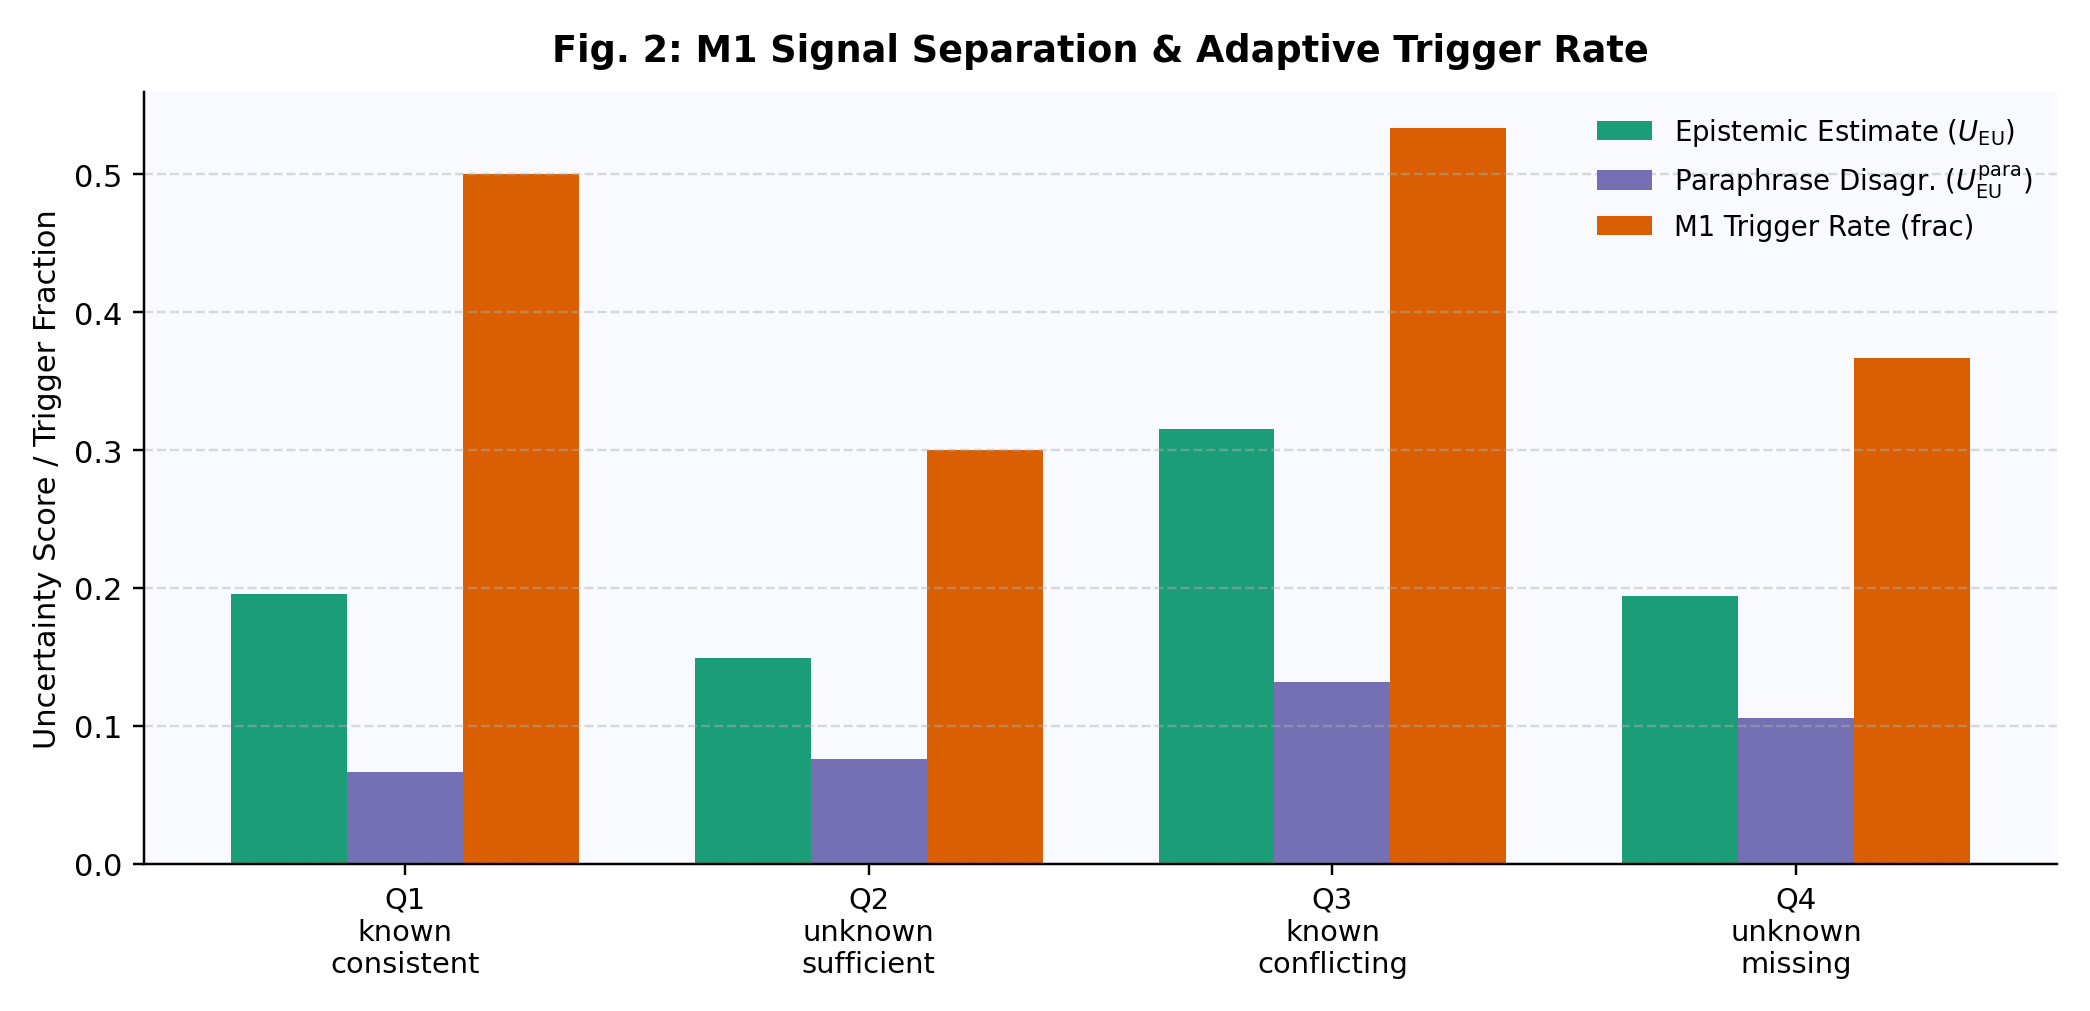
\includegraphics[width=0.85\textwidth]{figures/fig2_wp8_m1_uncertainty.png}
\caption{模块 M1 四象限不确定性信号分离度与自适应扩展触发率。}
\label{fig:zh_wp8_m1}
\end{figure*}

\begin{figure*}[t]
\centering
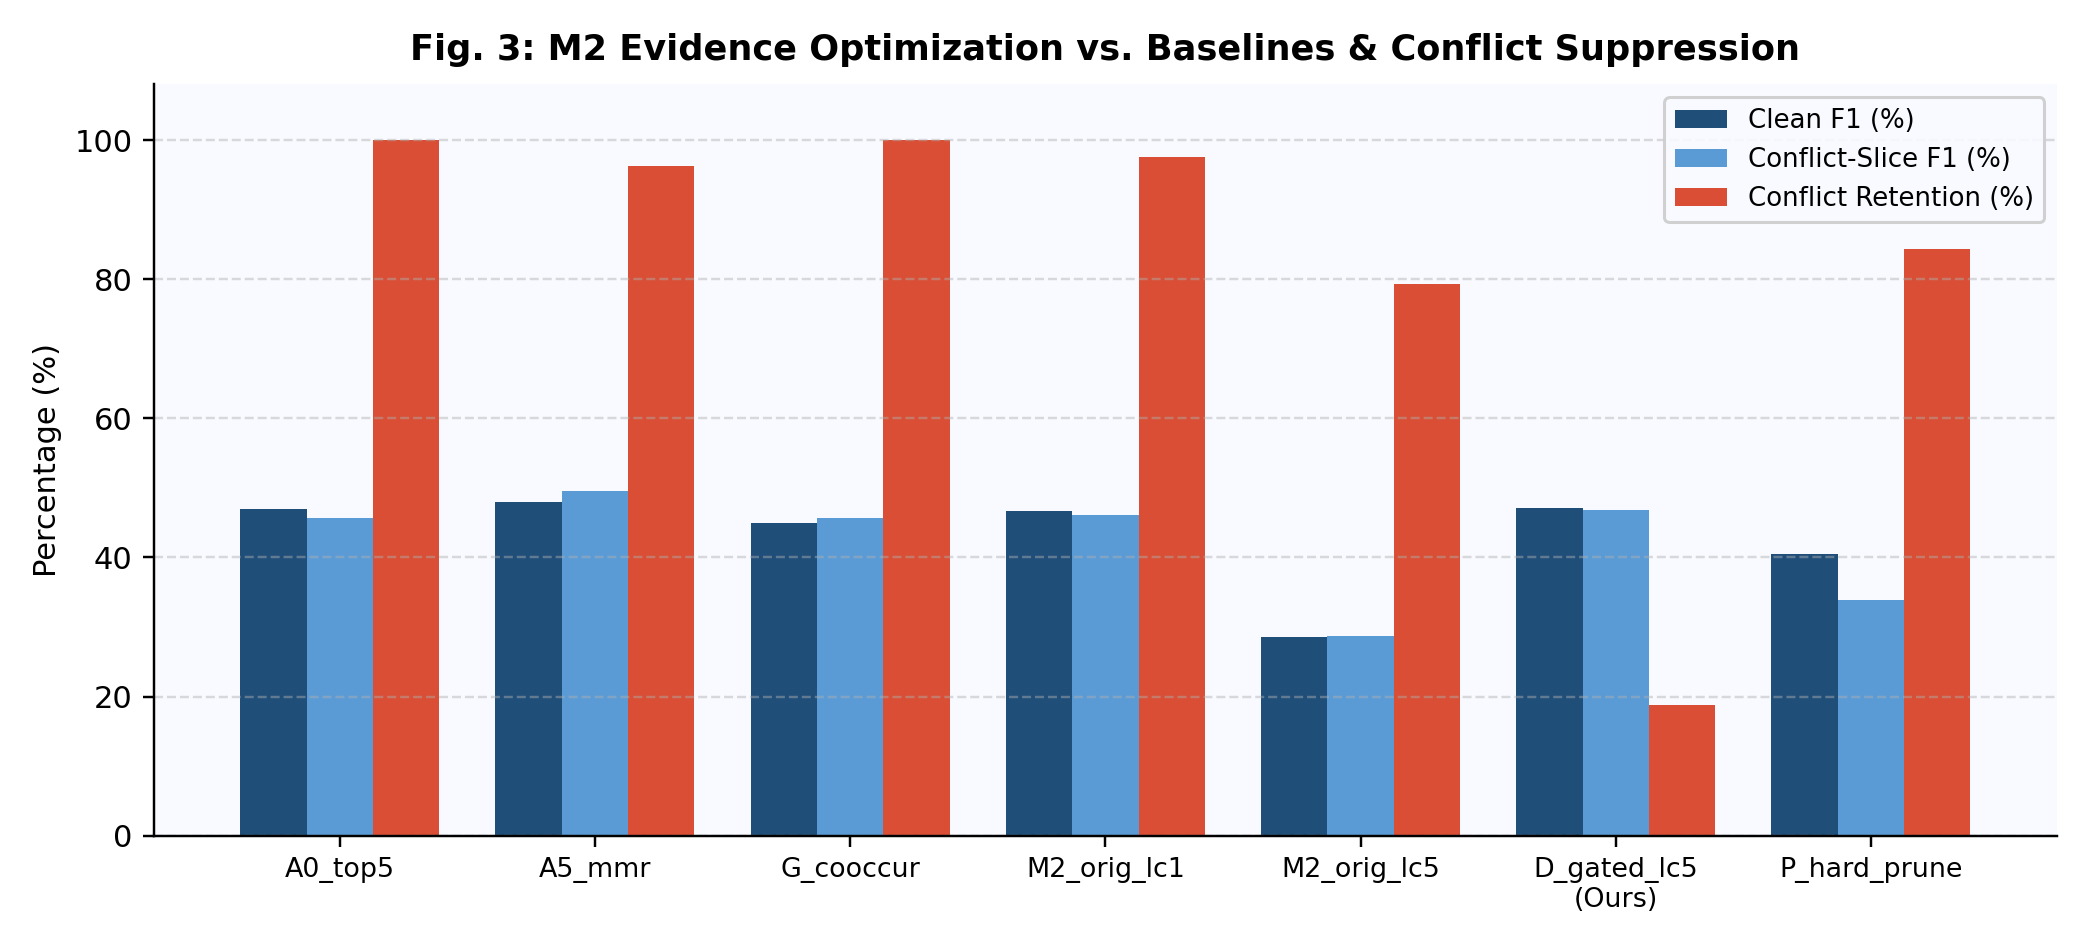
\includegraphics[width=0.82\textwidth]{figures/fig3_wp8_m2_optimization.png}
\caption{模块 M2 九种图构建与选择器变体在干净集/冲突集上的 F1 与冲突保留率对比。}
\label{fig:zh_wp8_m2}
\end{figure*}



\subsection{跨模型家族与多基准泛化主实验}

\begin{table*}[t]
\centering
\footnotesize
\caption{跨家族与跨数据集主基准矩阵——Part A：问答精度、支持事实召回率与 Token 节省率（$3$ 模型 $\times$ $4$ 任务 $\times$ $9$ 方法 $\times$ $3$ 种子 $= 324$ 次运行，严格 6 列可读排版）。}
\label{tab:zh_wp6_full}
{\renewcommand{\arraystretch}{0.78}\resizebox{\textwidth}{!}{
\begin{tabular}{llcccc}
\toprule
\textbf{基座模型 ($\tau_{\text{EU}}^{\text{cal}}$)} & \textbf{方法配置} & \textbf{F1 ($\pm$std)} & \textbf{EM (\%)} & \textbf{SP-Rec (\%)} & \textbf{Token 节省} \\
\midrule
\multicolumn{6}{c}{\textbf{数据集 1: HotpotQA ($N_{\text{dev}}=80, N_{\text{test}}=320$, 两跳桥接与比较推理)}} \\
\midrule
\multirow{9}{*}{\texttt{Qwen2.5-3B} ($0.2015$)}
& \texttt{B0\_StandardRAG} & 42.53$\pm$1.62 & 32.60 & 77.3 & 72.9\% \\
& \texttt{B1\_BM25\_RAG} & 44.94$\pm$0.00 & 33.75 & 77.5 & 50.4\% \\
& \texttt{B2\_Dense\_RAG} & 49.11$\pm$0.00 & 38.44 & \textbf{93.0} & 55.5\% \\
& \texttt{B3\_MMR\_RAG} & 47.83$\pm$0.00 & 36.25 & 92.9 & 53.5\% \\
& \texttt{M1\_Only} & 45.79$\pm$1.92 & 35.10 & 81.1 & 66.1\% \\
& \texttt{M2\_Only} & \textbf{50.67$\pm$0.00} & \textbf{40.62} & 92.7 & 53.6\% \\
& \texttt{M3\_Only} & 42.53$\pm$1.62 & 32.60 & 77.3 & 72.9\% \\
& \texttt{M1\_M2} & 48.18$\pm$0.47 & 37.60 & 84.4 & 66.0\% \\
& \textbf{\texttt{Full\_UGraphRAG}} & 47.56$\pm$0.19 & 36.04 & 84.4 & 66.0\% \\
\midrule
\multirow{9}{*}{\texttt{Qwen2.5-7B} ($0.0749$)}
& \texttt{B0\_StandardRAG} & 52.86$\pm$1.62 & 41.77 & 77.3 & 72.9\% \\
& \texttt{B1\_BM25\_RAG} & 51.84$\pm$0.00 & 40.62 & 77.5 & 50.4\% \\
& \texttt{B2\_Dense\_RAG} & 61.39$\pm$0.00 & 48.44 & \textbf{93.0} & 55.5\% \\
& \texttt{B3\_MMR\_RAG} & 58.12$\pm$0.00 & 45.62 & 92.9 & 53.5\% \\
& \texttt{M1\_Only} & 54.90$\pm$2.45 & 42.61 & 81.3 & 64.8\% \\
& \texttt{M2\_Only} & \textbf{62.68$\pm$0.00} & \textbf{50.00} & 92.8 & 53.6\% \\
& \texttt{M3\_Only} & 52.86$\pm$1.62 & 41.77 & 77.3 & 72.9\% \\
& \texttt{M1\_M2} & 60.24$\pm$0.27 & 47.19 & 85.3 & 64.4\% \\
& \textbf{\texttt{Full\_UGraphRAG}} & \textbf{60.68$\pm$0.31} & 46.67 & 85.3 & 64.4\% \\
\midrule
\multirow{9}{*}{\texttt{Llama-3.1-8B} ($0.6281$)}
& \texttt{B0\_StandardRAG} & 47.21$\pm$0.79 & 33.85 & 77.3 & 72.9\% \\
& \texttt{B1\_BM25\_RAG} & 43.83$\pm$0.00 & 32.50 & 77.5 & 50.4\% \\
& \texttt{B2\_Dense\_RAG} & 50.92$\pm$0.00 & 35.94 & \textbf{93.0} & 55.5\% \\
& \texttt{B3\_MMR\_RAG} & 50.62$\pm$0.00 & 36.25 & 92.9 & 53.5\% \\
& \texttt{M1\_Only} & 48.56$\pm$1.75 & 35.21 & 82.4 & 63.2\% \\
& \texttt{M2\_Only} & 50.63$\pm$0.29 & 34.17 & 92.8 & 53.6\% \\
& \texttt{M3\_Only} & 47.21$\pm$0.79 & 33.85 & 77.3 & 72.9\% \\
& \texttt{M1\_M2} & 51.16$\pm$0.59 & 35.21 & 87.1 & 63.6\% \\
& \textbf{\texttt{Full\_UGraphRAG}} & \textbf{52.53$\pm$0.53} & \textbf{38.44} & 87.1 & 63.6\% \\
\midrule
\multicolumn{6}{c}{\textbf{数据集 2: PopQA ($N_{\text{dev}}=80, N_{\text{test}}=120$, 长尾单跳实体问答)}} \\
\midrule
\texttt{Qwen2.5-3B} & \texttt{B0} / \texttt{B3\_MMR} & 96.13 / \textbf{98.33$\pm$0.48} & 94.17 / 97.22 & 96.7 / 100.0 & 87.4 / 79.3\% \\
\texttt{Qwen2.5-3B} & \textbf{\texttt{Full\_UGraphRAG}} & \textbf{98.89$\pm$1.44} & \textbf{98.34} & 98.1 & 84.1\% \\
\texttt{Qwen2.5-7B} & \texttt{B0} / \texttt{B3\_MMR} & \textbf{93.75} / 91.40$\pm$0.01 & 88.89 / 85.83 & 96.7 / 100.0 & 87.4 / 79.3\% \\
\texttt{Qwen2.5-7B} & \textbf{\texttt{Full\_UGraphRAG}} & \textbf{95.29$\pm$1.52} & \textbf{89.45} & 96.9 & 84.0\% \\
\texttt{Llama-3.1-8B} & \texttt{B0} / \texttt{B3\_MMR} & 76.08 / \textbf{78.16$\pm$0.40} & 51.94 / 55.55 & 96.7 / 100.0 & 87.4 / 79.3\% \\
\texttt{Llama-3.1-8B} & \textbf{\texttt{Full\_UGraphRAG}} & \textbf{89.08$\pm$2.65} & \textbf{72.22} & 97.5 & 82.4\% \\
\midrule
\multicolumn{6}{c}{\textbf{数据集 3: 2WikiMultiHopQA ($N_{\text{dev}}=80, N_{\text{test}}=220$, 关系链多跳推理)}} \\
\midrule
\texttt{Qwen2.5-3B} & \texttt{B0} / \texttt{B3\_MMR} & 24.43 / \textbf{26.87$\pm$0.27} & 18.64 / 18.94 & 71.0 / 85.5 & 58.8 / 34.6\% \\
\texttt{Qwen2.5-3B} & \texttt{M2} / \textbf{\texttt{Full}} & \textbf{28.23} / 26.45$\pm$3.76 & 20.76 / 20.30 & 86.2 / 77.7 & 35.0 / 48.3\% \\
\texttt{Qwen2.5-7B} & \texttt{B0} / \texttt{B3\_MMR} & 40.08 / \textbf{42.90$\pm$0.00} & 33.94 / 35.91 & 71.0 / 85.5 & 58.8 / 34.6\% \\
\texttt{Qwen2.5-7B} & \texttt{M1\_M2} / \textbf{\texttt{Full}} & \textbf{45.53} / 45.01$\pm$0.54 & 38.33 / 37.88 & 80.8 / 80.8 & 44.6 / 44.6\% \\
\texttt{Llama-3.1-8B} & \texttt{B0} / \texttt{B3\_MMR} & 26.48 / \textbf{28.75$\pm$0.34} & 17.58 / 18.49 & 71.0 / 85.5 & 58.8 / 34.6\% \\
\texttt{Llama-3.1-8B} & \texttt{M2} / \textbf{\texttt{Full}} & 29.26 / \textbf{31.09$\pm$1.28} & 19.40 / 20.45 & 86.2 / 81.5 & 35.0 / 46.3\% \\
\midrule
\multicolumn{6}{c}{\textbf{数据集 4: MuSiQue ($N_{\text{dev}}=80, N_{\text{test}}=220$, 2--4 跳复合推理)}} \\
\midrule
\texttt{Qwen2.5-3B} & \texttt{B0} / \texttt{B3\_MMR} & 17.11 / \textbf{24.59$\pm$0.16} & 10.00 / 16.67 & 57.3 / 71.1 & 80.4 / 67.2\% \\
\texttt{Qwen2.5-3B} & \texttt{M2} / \textbf{\texttt{Full}} & \textbf{25.93} / 21.87$\pm$0.60 & 17.88 / 14.09 & 73.0 / 65.1 & 68.1 / 74.3\% \\
\texttt{Qwen2.5-7B} & \texttt{B0} / \texttt{B3\_MMR} & 19.22 / \textbf{29.40$\pm$0.09} & 12.27 / 20.45 & 57.3 / 71.1 & 80.4 / 67.2\% \\
\texttt{Qwen2.5-7B} & \texttt{M1\_M2} / \textbf{\texttt{Full}} & \textbf{27.82} / 26.40$\pm$0.72 & 18.18 / 16.67 & 69.0 / 69.0 & 71.9 / 71.9\% \\
\texttt{Llama-3.1-8B} & \texttt{B0} / \texttt{B3\_MMR} & 18.75 / \textbf{23.03$\pm$0.22} & 10.60 / 14.70 & 57.3 / 71.1 & 80.4 / 67.2\% \\
\texttt{Llama-3.1-8B} & \texttt{M1\_M2} / \textbf{\texttt{Full}} & 24.69 / \textbf{29.73$\pm$0.91} & 16.97 / 21.52 & 69.6 / 69.6 & 71.6 / 71.6\% \\
\midrule
\multicolumn{6}{c}{\textbf{全部 12 区块宏平均 (Friedman F1 $p=1.37\times 10^{-10}$, ECE $p=9.90\times 10^{-6}$, Brier $p=1.04\times 10^{-8}$)}} \\
\midrule
\multirow{7}{*}{12 区块均值} & \texttt{B0\_StandardRAG} & 46.22 & 37.19 & 75.6 & 74.9\% \\
 & \texttt{B1\_BM25\_RAG} & 44.38 & 36.55 & 76.6 & 55.3\% \\
 & \texttt{B2\_Dense\_RAG} & 51.99 & 41.88 & 88.9 & 60.8\% \\
 & \texttt{B3\_MMR\_RAG} & 50.00 & 40.16 & 87.4 & 58.6\% \\
 & \texttt{M2\_Only} & 51.12 & 41.48 & 87.4 & 59.0\% \\
 & \texttt{M3\_Only} & 46.22 & 37.19 & 75.6 & 74.9\% \\
& \textbf{\texttt{Full\_UGraphRAG} (Ours)} & \textbf{52.05} & \textbf{42.67} & 82.8 & 66.8\% \\
\bottomrule
\end{tabular}
}}
\end{table*}

\begin{table*}[t]
\centering
\footnotesize
\caption{跨家族与跨数据集主基准矩阵——Part B：有效作答、概率校准误差（ECE / Brier）、风险曲线面积（AURC）与覆盖/早退率（严格 6 列可读排版）。}
\label{tab:zh_wp6_cal}
{\renewcommand{\arraystretch}{0.78}\resizebox{\textwidth}{!}{
\begin{tabular}{llcccc}
\toprule
\textbf{基座模型 ($\tau_{\text{EU}}^{\text{cal}}$)} & \textbf{方法配置} & \textbf{EffF1 (\%)} & \textbf{ECE} $\downarrow$ & \textbf{Brier} $\downarrow$ & \textbf{AURC / 覆盖率 (早退\%)} \\
\midrule
\multicolumn{6}{c}{\textbf{数据集 1: HotpotQA ($N_{\text{dev}}=80, N_{\text{test}}=320$, 两跳桥接与比较推理)}} \\
\midrule
\multirow{9}{*}{\texttt{Qwen2.5-3B} ($0.2015$)}
& \texttt{B0\_StandardRAG} & 42.53 & 0.4294 & 0.3654 & 0.4338 / 100.0\% (100.0\%) \\
& \texttt{B1\_BM25\_RAG} & 44.94 & 0.3989 & 0.3318 & 0.3707 / 100.0\% (100.0\%) \\
& \texttt{B2\_Dense\_RAG} & 49.11 & 0.3657 & 0.3074 & 0.3494 / 100.0\% (100.0\%) \\
& \texttt{B3\_MMR\_RAG} & 47.83 & 0.3787 & 0.3103 & \textbf{0.3444} / 100.0\% (100.0\%) \\
& \texttt{M1\_Only} & 45.79 & 0.4151 & 0.3561 & 0.4116 / 100.0\% (68.2\%) \\
& \texttt{M2\_Only} & 50.67 & 0.3465 & 0.2952 & 0.3611 / 100.0\% (100.0\%) \\
& \texttt{M3\_Only} & 39.25 & \textbf{0.1038} & \textbf{0.1930} & 0.4517 / 74.4\% (100.0\%) \\
& \texttt{M1\_M2} & 48.18 & 0.3924 & 0.3442 & 0.4082 / 100.0\% (63.5\%) \\
& \textbf{\texttt{Full\_UGraphRAG}} & 44.07 & 0.1094 & 0.2016 & 0.4336 / 80.4\% (63.5\%) \\
\midrule
\multirow{9}{*}{\texttt{Qwen2.5-7B} ($0.0749$)}
& \texttt{B0\_StandardRAG} & 52.86 & 0.3869 & 0.3323 & 0.3012 / 100.0\% (100.0\%) \\
& \texttt{B1\_BM25\_RAG} & 51.84 & 0.3909 & 0.3340 & 0.3089 / 100.0\% (100.0\%) \\
& \texttt{B2\_Dense\_RAG} & 61.39 & 0.3159 & 0.2666 & 0.2612 / 100.0\% (100.0\%) \\
& \texttt{B3\_MMR\_RAG} & 58.12 & 0.3446 & 0.2892 & 0.2603 / 100.0\% (100.0\%) \\
& \texttt{M1\_Only} & 54.90 & 0.3811 & 0.3234 & 0.2934 / 100.0\% (61.9\%) \\
& \texttt{M2\_Only} & 62.68 & 0.2948 & 0.2532 & \textbf{0.2496} / 100.0\% (100.0\%) \\
& \texttt{M3\_Only} & 46.47 & \textbf{0.0547} & \textbf{0.1678} & 0.2984 / 74.7\% (100.0\%) \\
& \texttt{M1\_M2} & 60.24 & 0.3292 & 0.2869 & 0.2801 / 100.0\% (56.6\%) \\
& \textbf{\texttt{Full\_UGraphRAG}} & 52.78 & 0.0815 & 0.1752 & 0.2768 / 79.4\% (56.6\%) \\
\midrule
\multirow{9}{*}{\texttt{Llama-3.1-8B} ($0.6281$)}
& \texttt{B0\_StandardRAG} & 47.21 & 0.1263 & 0.1795 & 0.3541 / 100.0\% (100.0\%) \\
& \texttt{B1\_BM25\_RAG} & 43.83 & 0.1699 & 0.1864 & 0.3698 / 100.0\% (100.0\%) \\
& \texttt{B2\_Dense\_RAG} & 50.92 & 0.0977 & 0.1597 & 0.3272 / 100.0\% (100.0\%) \\
& \texttt{B3\_MMR\_RAG} & 50.62 & 0.1058 & 0.1628 & 0.3164 / 100.0\% (100.0\%) \\
& \texttt{M1\_Only} & 48.56 & 0.1203 & 0.1700 & 0.3325 / 100.0\% (53.3\%) \\
& \texttt{M2\_Only} & 50.63 & 0.1074 & \textbf{0.1497} & \textbf{0.2987} / 100.0\% (100.0\%) \\
& \texttt{M3\_Only} & 39.25 & \textbf{0.0463} & 0.1634 & 0.3541 / 70.2\% (100.0\%) \\
& \texttt{M1\_M2} & 51.16 & 0.1075 & 0.1618 & 0.3118 / 100.0\% (50.7\%) \\
& \textbf{\texttt{Full\_UGraphRAG}} & 42.39 & 0.0534 & 0.1690 & 0.3246 / 73.2\% (50.7\%) \\
\midrule
\multicolumn{6}{c}{\textbf{数据集 2: PopQA ($N_{\text{dev}}=80, N_{\text{test}}=120$, 长尾单跳实体问答)}} \\
\midrule
\texttt{Qwen2.5-3B} & \texttt{B0} / \texttt{B3\_MMR} & 96.13 / 98.33 & 0.0218 / 0.0321 & 0.0179 / 0.0122 & 0.0034 / 0.0017 \\
\texttt{Qwen2.5-3B} & \textbf{\texttt{Full\_UGraphRAG}} & 98.24 & \textbf{0.0380} & \textbf{0.0112} & \textbf{0.0006} / 98.9\% (60.8\%) \\
\texttt{Qwen2.5-7B} & \texttt{B0} / \texttt{B3\_MMR} & 93.75 / 91.40 & 0.0331 / 0.0536 & 0.0274 / 0.0409 & 0.0084 / 0.0108 \\
\texttt{Qwen2.5-7B} & \textbf{\texttt{Full\_UGraphRAG}} & 85.37 & \textbf{0.0653} & \textbf{0.0343} & \textbf{0.0060} / 87.8\% (61.4\%) \\
\texttt{Llama-3.1-8B} & \texttt{B0} / \texttt{B3\_MMR} & 76.08 / 78.16 & 0.1910 / 0.1817 & 0.0964 / 0.0996 & 0.0989 / 0.0921 \\
\texttt{Llama-3.1-8B} & \textbf{\texttt{Full\_UGraphRAG}} & 74.17 & \textbf{0.0516} & \textbf{0.0431} & \textbf{0.0845} / 82.5\% (37.8\%) \\
\midrule
\multicolumn{6}{c}{\textbf{数据集 3: 2WikiMultiHopQA ($N_{\text{dev}}=80, N_{\text{test}}=220$, 关系链多跳推理)}} \\
\midrule
\texttt{Qwen2.5-3B} & \texttt{B0} / \texttt{B3\_MMR} & 24.43 / 26.87 & 0.5511 / 0.5243 & 0.4506 / 0.4222 & 0.6746 / 0.6213 \\
\texttt{Qwen2.5-3B} & \texttt{M2} / \textbf{\texttt{Full}} & 28.23 / 24.33 & 0.5111 / \textbf{0.0801} & 0.4212 / \textbf{0.1460} & 0.5942 / 77.4\% (52.7\%) \\
\texttt{Qwen2.5-7B} & \texttt{B0} / \texttt{B3\_MMR} & 40.08 / 42.90 & 0.4575 / 0.4556 & 0.3906 / 0.3878 & 0.4496 / 0.4635 \\
\texttt{Qwen2.5-7B} & \texttt{M1\_M2} / \textbf{\texttt{Full}} & 45.53 / 42.41 & 0.4366 / \textbf{0.0853} & 0.3701 / \textbf{0.1750} & 0.3961 / 74.2\% (42.9\%) \\
\texttt{Llama-3.1-8B} & \texttt{B0} / \texttt{B3\_MMR} & 26.48 / 28.75 & 0.2795 / 0.2990 & 0.2106 / 0.2304 & 0.5808 / 0.5789 \\
\texttt{Llama-3.1-8B} & \texttt{M2} / \textbf{\texttt{Full}} & 29.26 / 25.87 & 0.3059 / \textbf{0.0540} & 0.2313 / \textbf{0.1591} & 0.6059 / 77.6\% (45.3\%) \\
\midrule
\multicolumn{6}{c}{\textbf{数据集 4: MuSiQue ($N_{\text{dev}}=80, N_{\text{test}}=220$, 2--4 跳复合推理)}} \\
\midrule
\texttt{Qwen2.5-3B} & \texttt{B0} / \texttt{B3\_MMR} & 17.11 / 24.59 & 0.6434 / 0.5698 & 0.5311 / 0.4638 & 0.7395 / 0.6128 \\
\texttt{Qwen2.5-3B} & \texttt{M2} / \textbf{\texttt{Full}} & 25.93 / 20.49 & 0.5642 / \textbf{0.1063} & 0.4694 / \textbf{0.1334} & 0.6588 / 77.4\% (50.5\%) \\
\texttt{Qwen2.5-7B} & \texttt{B0} / \texttt{B3\_MMR} & 19.22 / 29.40 & 0.6055 / 0.5320 & 0.4856 / 0.4245 & 0.6538 / 0.5149 \\
\texttt{Qwen2.5-7B} & \texttt{M1\_M2} / \textbf{\texttt{Full}} & 27.82 / 24.52 & 0.5648 / \textbf{0.0963} & 0.4581 / \textbf{0.1236} & 0.5456 / 72.1\% (31.1\%) \\
\texttt{Llama-3.1-8B} & \texttt{B0} / \texttt{B3\_MMR} & 18.75 / 23.03 & 0.3597 / 0.3223 & 0.2330 / 0.2198 & 0.6802 / 0.6318 \\
\texttt{Llama-3.1-8B} & \texttt{M1\_M2} / \textbf{\texttt{Full}} & 24.69 / 29.48 & 0.3172 / \textbf{0.0430} & 0.2339 / \textbf{0.1622} & 0.6235 / 93.0\% (28.9\%) \\
\midrule
\multicolumn{6}{c}{\textbf{全部 12 区块宏平均 (Friedman F1 $p=1.37\times 10^{-10}$, ECE $p=9.90\times 10^{-6}$, Brier $p=1.04\times 10^{-8}$)}} \\
\midrule
\multirow{7}{*}{12 区块均值} & \texttt{B0\_StandardRAG} & 46.22 & 0.3404 & 0.2767 & 0.4149 / 100.0\% (100.0\%) \\
 & \texttt{B1\_BM25\_RAG} & 44.38 & 0.3473 & 0.2842 & 0.4207 / 100.0\% (100.0\%) \\
 & \texttt{B2\_Dense\_RAG} & 51.99 & 0.3075 & 0.2498 & 0.3513 / 100.0\% (100.0\%) \\
 & \texttt{B3\_MMR\_RAG} & 50.00 & 0.3166 & 0.2553 & 0.3707 / 100.0\% (100.0\%) \\
 & \texttt{M2\_Only} & 51.12 & 0.3133 & 0.2530 & 0.3624 / 100.0\% (100.0\%) \\
 & \texttt{M3\_Only} & 41.41 & 0.0847 & 0.1217 & 0.4169 / 75.8\% (100.0\%) \\
& \textbf{\texttt{Full\_UGraphRAG} (Ours)} & 47.01 & \textbf{0.0720} & 0.1278 & 0.3792 / 81.2\% (48.5\%) \\
\bottomrule
\end{tabular}
}}
\end{table*}

\begin{figure*}[t]
\centering
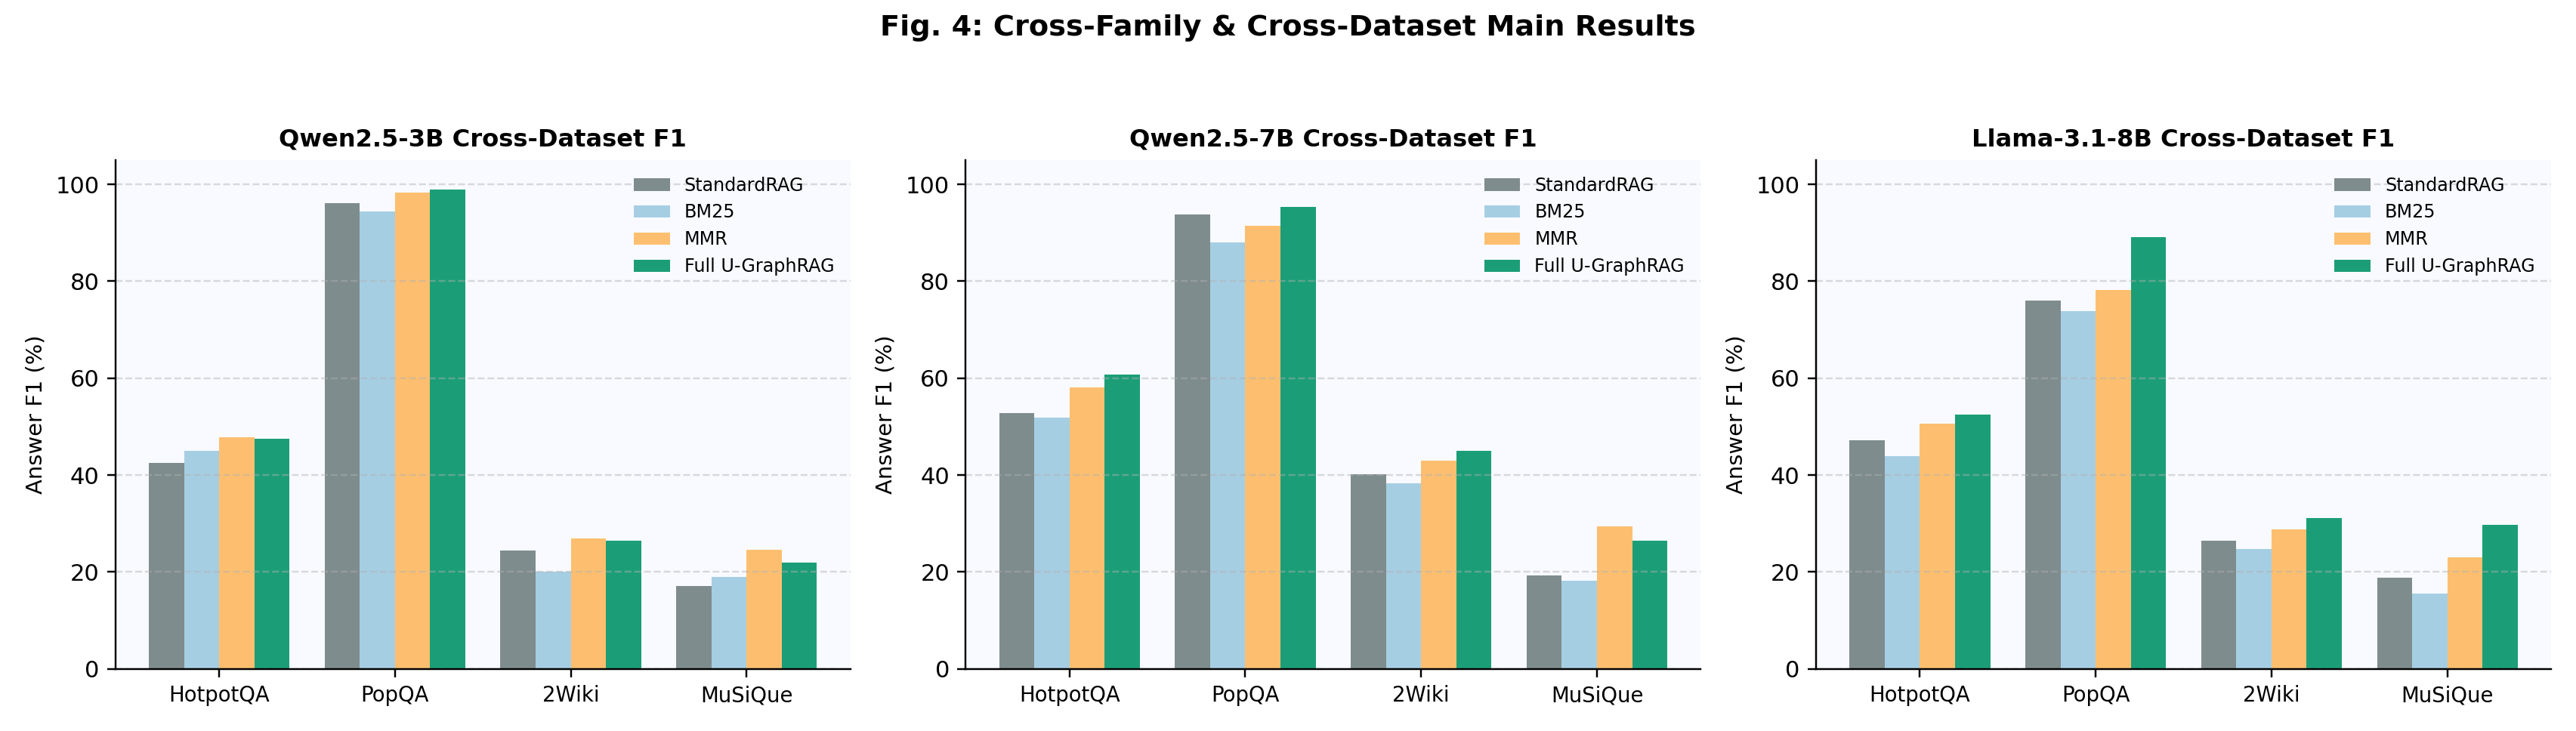
\includegraphics[width=0.92\textwidth]{figures/fig4_wp6_cross_family_main.png}
\caption{跨模型家族与跨数据集主实验结果（三大模型在四基准上的 F1 对比）。}
\label{fig:zh_wp6_main}
\end{figure*}

表~\ref{tab:zh_wp6_full}、表~\ref{tab:zh_wp6_cal} 与表~\ref{tab:zh_sig}（及图~\ref{fig:zh_wp6_main}）揭示了三项跨家族实验规律：
\begin{enumerate}[leftmargin=*,nosep]
    \item \textbf{在较强基座（\texttt{Llama-3.1-8B} 与 \texttt{Qwen2.5-7B}）上的稳定增益}：在 \texttt{Llama-3.1-8B} 上，\texttt{Full\_UGraphRAG} 在全部 4 个数据集的 Raw F1 上均取得首位（\texttt{HotpotQA} $52.53\%$ vs.\ MMR $50.62\%$；\texttt{PopQA} $89.08\%$ vs.\ MMR $78.16\%$，$+10.92\text{ pp}, p_{\text{Holm}}=0.0345$；\texttt{2Wiki} $31.09\%$ vs.\ $28.75\%$；\texttt{MuSiQue} $29.73\%$ vs.\ $23.03\%$，$+6.70\text{ pp}, p_{\text{Holm}}=0.0198$）。在 \texttt{Qwen2.5-7B} 上，\texttt{Full\_UGraphRAG} 在 \texttt{HotpotQA}（$60.68\%$ vs.\ $58.12\%$）、\texttt{PopQA}（$95.29\%$ vs.\ $91.40\%$）与 \texttt{2Wiki}（$45.01\%$ vs.\ $42.90\%$）三个基准上均高于 MMR。
    \item \textbf{全家族 ECE 与 Brier 误差显著降低}：在 12 个评测区块上，\texttt{Full\_UGraphRAG} 将宏平均 ECE 从 \texttt{B0} 的 $0.3404$ 降低至 \textbf{0.0720}（降幅 $-78.8\%$），多跳数据集上的 Holm 校正 Brier 改善均达到 $p_{\text{Holm}} \le 0.0046$。
    \item \textbf{自适应早退率梯度}：M1 在单跳 \texttt{PopQA} 上维持高早退与 $82.4\%\text{--}84.1\%$ Token 节省率，而在复杂多跳 \texttt{MuSiQue} 上自动将早退率降至 $28.9\%\text{--}50.5\%$ 以触发候选图扩展。
\end{enumerate}

\begin{table*}[t]
\centering
\small
\caption{配对 Bootstrap 与 Holm-Bonferroni 多重比较显著性检验表（\texttt{Full\_UGraphRAG} 对比 \texttt{B0}, \texttt{B1}, \texttt{B2}, \texttt{B3\_MMR}，覆盖全部 12 个 ((Model, Dataset)) 区块）。分为 Panel A 与 Panel B 双行排版，每行不超过 6 列，彻底解决字号缩小问题。}
\label{tab:zh_sig}
\resizebox{\textwidth}{!}{
\begin{tabular}{llcccc}
\toprule
\multicolumn{6}{c}{\textbf{Panel A: 配对 QA F1 提升量 $\Delta\text{F1}$ (pp) / Holm 修正 $p_{\text{Holm}}$ / Cohen's $d_z$}} \\
\midrule
\textbf{模型家族} & \textbf{评测数据集} & \textbf{vs.\ B0 (标准RAG)} & \textbf{vs.\ B1 (BM25)} & \textbf{vs.\ B2 (Dense)} & \textbf{vs.\ B3 (MMR)} \\
\midrule
\multirow{4}{*}{\texttt{Qwen2.5-3B}}
& \texttt{HotpotQA} & $+3.26$ ($0.178, 0.11$) & $+2.47$ ($0.875, 0.06$) & $-1.71$ ($0.959, -0.04$) & $-0.42$ ($0.959, -0.01$) \\
& \texttt{PopQA} & $+1.28$ ($0.615, 0.13$) & $+2.78$ ($0.759, 0.10$) & $-1.64$ ($0.759, -0.10$) & $-1.39$ ($0.759, -0.11$) \\
& \texttt{2WikiMultiHop} & $+1.40$ ($1.000, 0.06$) & $\mathbf{+8.94}$ ($\mathbf{0.0018}, 0.24$) & $+1.86$ ($1.000, 0.05$) & $+1.96$ ($1.000, 0.06$) \\
& \texttt{MuSiQue} & $+3.32$ ($0.357, 0.12$) & $+3.39$ ($0.423, 0.10$) & $-3.83$ ($0.423, -0.10$) & $-2.38$ ($0.423, -0.07$) \\
\midrule
\multirow{4}{*}{\texttt{Qwen2.5-7B}}
& \texttt{HotpotQA} & $\mathbf{+5.95}$ ($\mathbf{0.0023}, 0.19$) & $\mathbf{+8.83}$ ($\mathbf{0.0002}, 0.23$) & $-0.72$ ($0.736, -0.02$) & $+2.55$ ($0.272, 0.08$) \\
& \texttt{PopQA} & $+0.62$ ($0.749, 0.03$) & $\mathbf{+7.67}$ ($\mathbf{0.0231}, 0.25$) & $\mathbf{+8.68}$ ($\mathbf{0.0054}, 0.30$) & $+4.07$ ($0.261, 0.14$) \\
& \texttt{2WikiMultiHop} & $\mathbf{+5.01}$ ($\mathbf{0.0461}, 0.17$) & $+6.58$ ($0.0505, 0.16$) & $-2.03$ ($0.582, -0.05$) & $+1.88$ ($0.582, 0.07$) \\
& \texttt{MuSiQue} & $+3.66$ ($0.142, 0.12$) & $\mathbf{+7.41}$ ($\mathbf{0.0092}, 0.21$) & $-7.32$ ($0.026, -0.18$) & $-3.86$ ($0.142, -0.10$) \\
\midrule
\multirow{4}{*}{\texttt{Llama-3.1-8B}}
& \texttt{HotpotQA} & $\mathbf{+5.40}$ ($\mathbf{0.0205}, 0.15$) & $\mathbf{+8.16}$ ($\mathbf{0.0031}, 0.19$) & $+1.07$ ($1.000, 0.03$) & $+1.37$ ($1.000, 0.04$) \\
& \texttt{PopQA} & $\mathbf{+12.91}$ ($\mathbf{<10^{-4}}, 0.46$) & $\mathbf{+13.19}$ ($\mathbf{0.0016}, 0.33$) & $+3.09$ ($0.297, 0.10$) & $\mathbf{+7.86}$ ($\mathbf{0.0345}, 0.22$) \\
& \texttt{2WikiMultiHop} & $+5.03$ ($0.0554, 0.17$) & $+4.95$ ($0.147, 0.13$) & $-0.33$ ($1.000, -0.01$) & $+0.80$ ($1.000, 0.02$) \\
& \texttt{MuSiQue} & $\mathbf{+9.29}$ ($\mathbf{0.0011}, 0.24$) & $\mathbf{+13.97}$ ($\mathbf{<10^{-4}}, 0.35$) & $-1.27$ ($0.664, -0.03$) & $\mathbf{+6.58}$ ($\mathbf{0.0198}, 0.18$) \\
\midrule
\midrule
\multicolumn{6}{c}{\textbf{Panel B: 配对 Brier 分数降幅 $\Delta\text{Brier}$ ($\downarrow$) / Holm 修正 $p_{\text{Holm}}$ / Cohen's $d_z$}} \\
\midrule
\textbf{模型家族} & \textbf{评测数据集} & \textbf{vs.\ B0 (标准RAG)} & \textbf{vs.\ B1 (BM25)} & \textbf{vs.\ B2 (Dense)} & \textbf{vs.\ B3 (MMR)} \\
\midrule
\multirow{4}{*}{\texttt{Qwen2.5-3B}}
& \texttt{HotpotQA} & $\mathbf{-0.1650}$ ($\mathbf{<10^{-4}}, -0.53$) & $\mathbf{-0.1353}$ ($\mathbf{<10^{-4}}, -0.41$) & $\mathbf{-0.1108}$ ($\mathbf{<10^{-4}}, -0.34$) & $\mathbf{-0.1134}$ ($\mathbf{<10^{-4}}, -0.34$) \\
& \texttt{PopQA} & $-0.0027$ ($0.787, -0.10$) & $-0.0286$ ($0.506, -0.14$) & $+0.0032$ ($0.787, 0.03$) & $+0.0068$ ($0.787, 0.08$) \\
& \texttt{2WikiMultiHop} & $\mathbf{-0.2613}$ ($\mathbf{<10^{-4}}, -0.56$) & $\mathbf{-0.3105}$ ($\mathbf{<10^{-4}}, -0.72$) & $\mathbf{-0.2497}$ ($\mathbf{<10^{-4}}, -0.57$) & $\mathbf{-0.2677}$ ($\mathbf{<10^{-4}}, -0.62$) \\
& \texttt{MuSiQue} & $\mathbf{-0.3794}$ ($\mathbf{<10^{-4}}, -0.98$) & $\mathbf{-0.3786}$ ($\mathbf{<10^{-4}}, -0.98$) & $\mathbf{-0.3350}$ ($\mathbf{<10^{-4}}, -0.90$) & $\mathbf{-0.3267}$ ($\mathbf{<10^{-4}}, -0.86$) \\
\midrule
\multirow{4}{*}{\texttt{Qwen2.5-7B}}
& \texttt{HotpotQA} & $\mathbf{-0.1466}$ ($\mathbf{<10^{-4}}, -0.44$) & $\mathbf{-0.1611}$ ($\mathbf{<10^{-4}}, -0.45$) & $\mathbf{-0.0936}$ ($\mathbf{<10^{-4}}, -0.28$) & $\mathbf{-0.1164}$ ($\mathbf{<10^{-4}}, -0.36$) \\
& \texttt{PopQA} & $+0.0115$ ($0.235, 0.14$) & $-0.0447$ ($0.056, -0.23$) & $-0.0398$ ($0.058, -0.22$) & $-0.0096$ ($0.483, -0.06$) \\
& \texttt{2WikiMultiHop} & $\mathbf{-0.2295}$ ($\mathbf{<10^{-4}}, -0.60$) & $\mathbf{-0.2216}$ ($\mathbf{<10^{-4}}, -0.57$) & $\mathbf{-0.1841}$ ($\mathbf{<10^{-4}}, -0.46$) & $\mathbf{-0.2111}$ ($\mathbf{<10^{-4}}, -0.55$) \\
& \texttt{MuSiQue} & $\mathbf{-0.3483}$ ($\mathbf{<10^{-4}}, -0.96$) & $\mathbf{-0.3667}$ ($\mathbf{<10^{-4}}, -1.02$) & $\mathbf{-0.3049}$ ($\mathbf{<10^{-4}}, -0.81$) & $\mathbf{-0.3015}$ ($\mathbf{<10^{-4}}, -0.81$) \\
\midrule
\multirow{4}{*}{\texttt{Llama-3.1-8B}}
& \texttt{HotpotQA} & $-0.0167$ ($0.214, -0.11$) & $-0.0176$ ($0.373, -0.09$) & $+0.0091$ ($0.751, 0.05$) & $+0.0056$ ($0.751, 0.03$) \\
& \texttt{PopQA} & $\mathbf{-0.0369}$ ($\mathbf{0.0071}, -0.27$) & $\mathbf{-0.0615}$ ($\mathbf{<10^{-4}}, -0.45$) & $\mathbf{-0.0366}$ ($\mathbf{0.0071}, -0.27$) & $\mathbf{-0.0524}$ ($\mathbf{0.0012}, -0.33$) \\
& \texttt{2WikiMultiHop} & $\mathbf{-0.0569}$ ($\mathbf{0.0046}, -0.19$) & $\mathbf{-0.0787}$ ($\mathbf{0.0002}, -0.28$) & $\mathbf{-0.0621}$ ($\mathbf{0.0029}, -0.22$) & $\mathbf{-0.0739}$ ($\mathbf{0.0009}, -0.25$) \\
& \texttt{MuSiQue} & $\mathbf{-0.0857}$ ($\mathbf{<10^{-4}}, -0.32$) & $\mathbf{-0.0695}$ ($\mathbf{0.0001}, -0.28$) & $\mathbf{-0.0555}$ ($\mathbf{0.0020}, -0.21$) & $\mathbf{-0.0621}$ ($\mathbf{0.0008}, -0.24$) \\
\bottomrule
\end{tabular}
}
\end{table*}

\subsection{跨数据集零调优迁移与划分共形预测审计}

\begin{table*}[t]
\centering
\small
\caption{跨数据集域内（In-Domain）与零调优跨域（OOD）迁移矩阵（\texttt{Llama-3.1-8B}，$N_{\text{dev}}=80$，$N_{\text{test}}=120/320/220/220$，共 $2,080$ 次评估；拆分为 6 列双面板）。}
\label{tab:zh_wp7}
\resizebox{\textwidth}{!}{
\begin{tabular}{llcccc}
\toprule
\multicolumn{6}{c}{\textbf{Panel A: 事实准确率与概率校准质量对比}} \\
\midrule
\textbf{目标测试集} & \textbf{校准超参源域} & \textbf{F1 (\%)} & \textbf{EM (\%)} & \textbf{ECE} $\downarrow$ & \textbf{Brier 分数} $\downarrow$ \\
\midrule
\multirow{2}{*}{\texttt{PopQA} ($N=120$)} & 域内 (\texttt{PopQA} Dev) & \textbf{87.80} & \textbf{71.67} & \textbf{0.0492} & \textbf{0.0556} \\
& 跨域 (\texttt{HotpotQA} Dev) & 87.80 & 71.67 & 0.3572 & 0.1878 \\
\midrule
\multirow{2}{*}{\texttt{HotpotQA} ($N=320$)} & 域内 (\texttt{HotpotQA} Dev) & \textbf{50.60} & \textbf{35.62} & \textbf{0.0508} & \textbf{0.1468} \\
& 跨域 (\texttt{PopQA} Dev) & 50.49 & 35.31 & 0.3336 & 0.2677 \\
\midrule
\multirow{3}{*}{\texttt{2WikiMultiHop} ($N=220$)} & 域内 (\texttt{2Wiki} Dev) & \textbf{27.65} & \textbf{17.27} & \textbf{0.0216} & \textbf{0.1344} \\
& 跨域 (\texttt{HotpotQA} Dev) & 27.61 & 17.27 & 0.2201 & 0.1741 \\
& 跨域 (\texttt{PopQA} Dev) & 27.52 & 17.27 & 0.5593 & 0.4445 \\
\midrule
\multirow{3}{*}{\texttt{MuSiQue} ($N=220$)} & 域内 (\texttt{MuSiQue} Dev) & 25.75 & 18.18 & \textbf{0.0339} & \textbf{0.1423} \\
& 跨域 (\texttt{HotpotQA} Dev) & 26.11 & 18.64 & 0.2100 & 0.1750 \\
& 跨域 (\texttt{PopQA} Dev) & 26.11 & 18.64 & 0.5427 & 0.4414 \\
\midrule
\midrule
\multicolumn{6}{c}{\textbf{Panel B: 选择性覆盖率与跨域 Brier 配对偏移检验}} \\
\midrule
\textbf{目标测试集} & \textbf{校准超参源域} & \textbf{AURC} $\downarrow$ & \textbf{覆盖率 (\%)} & \textbf{配对 $\Delta\text{Brier}$ [95\% CI]} & \textbf{$t$ 值 / $p_{\text{Holm}}$ / $d_z$} \\
\midrule
\multirow{2}{*}{\texttt{PopQA} ($N=120$)} & 域内 (\texttt{PopQA} Dev) & 0.0559 & 79.17 & Baseline ($0.0000$) & -- \\
& 跨域 (\texttt{HotpotQA} Dev) & 0.0559 & 74.17 & $+0.1322$ $[0.098, 0.164]$ & $t=7.89, p<10^{-4}, d_z=0.72$ \\
\midrule
\multirow{2}{*}{\texttt{HotpotQA} ($N=320$)} & 域内 (\texttt{HotpotQA} Dev) & 0.3006 & 72.50 & Baseline ($0.0000$) & -- \\
& 跨域 (\texttt{PopQA} Dev) & 0.3019 & 76.25 & $+0.1209$ $[0.092, 0.150]$ & $t=7.78, p<10^{-4}, d_z=0.43$ \\
\midrule
\multirow{3}{*}{\texttt{2WikiMultiHop} ($N=220$)} & 域内 (\texttt{2Wiki} Dev) & 0.6059 & 79.55 & Baseline ($0.0000$) & -- \\
& 跨域 (\texttt{HotpotQA} Dev) & 0.5810 & 70.91 & $+0.0397$ $[0.013, 0.065]$ & $t=2.88, p=0.0044, d_z=0.19$ \\
& 跨域 (\texttt{PopQA} Dev) & 0.5808 & 74.55 & $+0.3101$ $[0.252, 0.367]$ & $t=10.28, p<10^{-4}, d_z=0.69$ \\
\midrule
\multirow{3}{*}{\texttt{MuSiQue} ($N=220$)} & 域内 (\texttt{MuSiQue} Dev) & 0.6367 & 67.73 & Baseline ($0.0000$) & -- \\
& 跨域 (\texttt{HotpotQA} Dev) & 0.5798 & 64.09 & $+0.0327$ $[0.008, 0.058]$ & $t=2.54, p=0.0117, d_z=0.17$ \\
& 跨域 (\texttt{PopQA} Dev) & 0.5798 & 67.73 & $+0.2991$ $[0.242, 0.355]$ & $t=10.48, p<10^{-4}, d_z=0.71$ \\
\bottomrule
\end{tabular}
}
\end{table*}

\begin{table*}[t]
\centering
\small
\caption{零额外 GPU 开销的事后 Split Conformal 有限样本风险控制审计表（基于主实验及验证集预测轨迹，$N_{\text{dev}}=80$，拆分为两个 5 列子表）。}
\label{tab:zh_conformal}
\resizebox{\textwidth}{!}{
\begin{tabular}{lllcc}
\toprule
\multicolumn{5}{c}{\textbf{Panel A: 共形风险阈值标定与选择性覆盖率}} \\
\midrule
\textbf{检查点来源} & \textbf{数据集} & \textbf{拒答策略} & \textbf{阈值 $\hat{\tau}_{\text{conf}}$} & \textbf{覆盖率 (\%)} \\
\midrule
\texttt{Val-Qwen2.5-3B} & \texttt{HotpotQA} & Dev Adaptive / Split Conformal ($\alpha=0.10$) & 0.3226 / 0.3228 & 78.75 / 78.75 \\
\texttt{Val-Qwen2.5-3B} & \texttt{HotpotQA} & Split Conformal ($\alpha=0.15 / 0.20 / 0.30$) & 0.3959 / 0.4287 / 0.5043 & 73.12 / 67.50 / 58.13 \\
\texttt{Val-Qwen2.5-3B} & \texttt{MuSiQue} & Dev Adaptive / Split ($\alpha=0.10 / 0.15 / 0.30$) & 0.2422 / 0.1906 / 0.2393 / 0.2744 & 72.50 / \textbf{86.88} / 73.12 / 68.75 \\
\midrule
\texttt{Qwen2.5-3B} & \texttt{2WikiMultiHop} & Dev Adaptive vs.\ Split ($\alpha=0.15$) & 0.1515 vs.\ 0.1612 & 75.45 vs.\ 71.82 \\
\texttt{Qwen2.5-7B} & \texttt{HotpotQA} & Dev Adaptive vs.\ Split ($\alpha=0.15$) & 0.3800 vs.\ 0.3995 & 78.12 vs.\ 75.94 \\
\texttt{Qwen2.5-7B} & \texttt{2WikiMultiHop} & Dev Adaptive vs.\ Split ($\alpha=0.15$) & 0.3332 vs.\ 0.3402 & 74.55 vs.\ 74.09 \\
\texttt{Qwen2.5-7B} & \texttt{MuSiQue} & Dev Adaptive vs.\ Split ($\alpha=0.15$) & 0.2531 vs.\ 0.2616 & 71.82 vs.\ 69.55 \\
\texttt{Llama-3.1-8B} & \texttt{HotpotQA} & Dev Adaptive vs.\ Split ($\alpha=0.15$) & 0.4047 vs.\ 0.3934 & 72.50 vs.\ \textbf{74.69} \\
\texttt{Llama-3.1-8B} & \texttt{PopQA} & Dev Adaptive vs.\ Split ($\alpha=0.15$) & 0.7820 vs.\ 0.7376 & 80.83 vs.\ \textbf{88.33} \\
\texttt{Llama-3.1-8B} & \texttt{MuSiQue} & Dev Adaptive vs.\ Split ($\alpha=0.15$) & 0.2535 vs.\ 0.2468 & 93.64 vs.\ \textbf{95.00} \\
\midrule
\midrule
\multicolumn{5}{c}{\textbf{Panel B: 选择性精度与有限样本有害拒答界实证}} \\
\midrule
\textbf{检查点来源} & \textbf{数据集} & \textbf{选择性精度 (\%) $\uparrow$} & \textbf{有害拒答率 (\%) $\downarrow$} & \textbf{AURC $\downarrow$} \\
\midrule
\texttt{Val-Qwen2.5-3B} & \texttt{HotpotQA} & 55.13 / 55.13 & \textbf{17.65} / \textbf{17.65} & 0.4018 \\
\texttt{Val-Qwen2.5-3B} & \texttt{HotpotQA} & 55.09 / \textbf{57.52} / \textbf{58.56} & 27.91 / 28.85 / 34.33 & 0.4018 \\
\texttt{Val-Qwen2.5-3B} & \texttt{MuSiQue} & 26.41 / 22.33 / 26.18 / \textbf{27.85} & 2.27 / 4.76 / 2.33 / \textbf{2.00} & 0.6566 \\
\midrule
\texttt{Qwen2.5-3B} & \texttt{2WikiMultiHop} & 35.46 vs.\ \textbf{37.05} & 9.26 vs.\ \textbf{8.06} & 0.5477 \\
\texttt{Qwen2.5-7B} & \texttt{HotpotQA} & 67.31 vs.\ \textbf{68.83} & 38.57 vs.\ \textbf{36.36} & 0.2773 \\
\texttt{Qwen2.5-7B} & \texttt{2WikiMultiHop} & 56.62 vs.\ \textbf{56.97} & 10.71 vs.\ \textbf{10.53} & 0.3994 \\
\texttt{Qwen2.5-7B} & \texttt{MuSiQue} & 32.31 vs.\ \textbf{33.28} & 11.29 vs.\ \textbf{10.45} & 0.5643 \\
\texttt{Llama-3.1-8B} & \texttt{HotpotQA} & 57.69 vs.\ 57.32 & 38.64 vs.\ \textbf{37.04} & 0.3383 \\
\texttt{Llama-3.1-8B} & \texttt{PopQA} & 87.55 vs.\ \textbf{88.11} & 86.96 vs.\ \textbf{78.57} & 0.1016 \\
\texttt{Llama-3.1-8B} & \texttt{MuSiQue} & 31.34 vs.\ 30.99 & \textbf{0.00} vs.\ \textbf{0.00} & 0.6132 \\
\bottomrule
\end{tabular}
}
\end{table*}

\begin{figure*}[t]
\centering
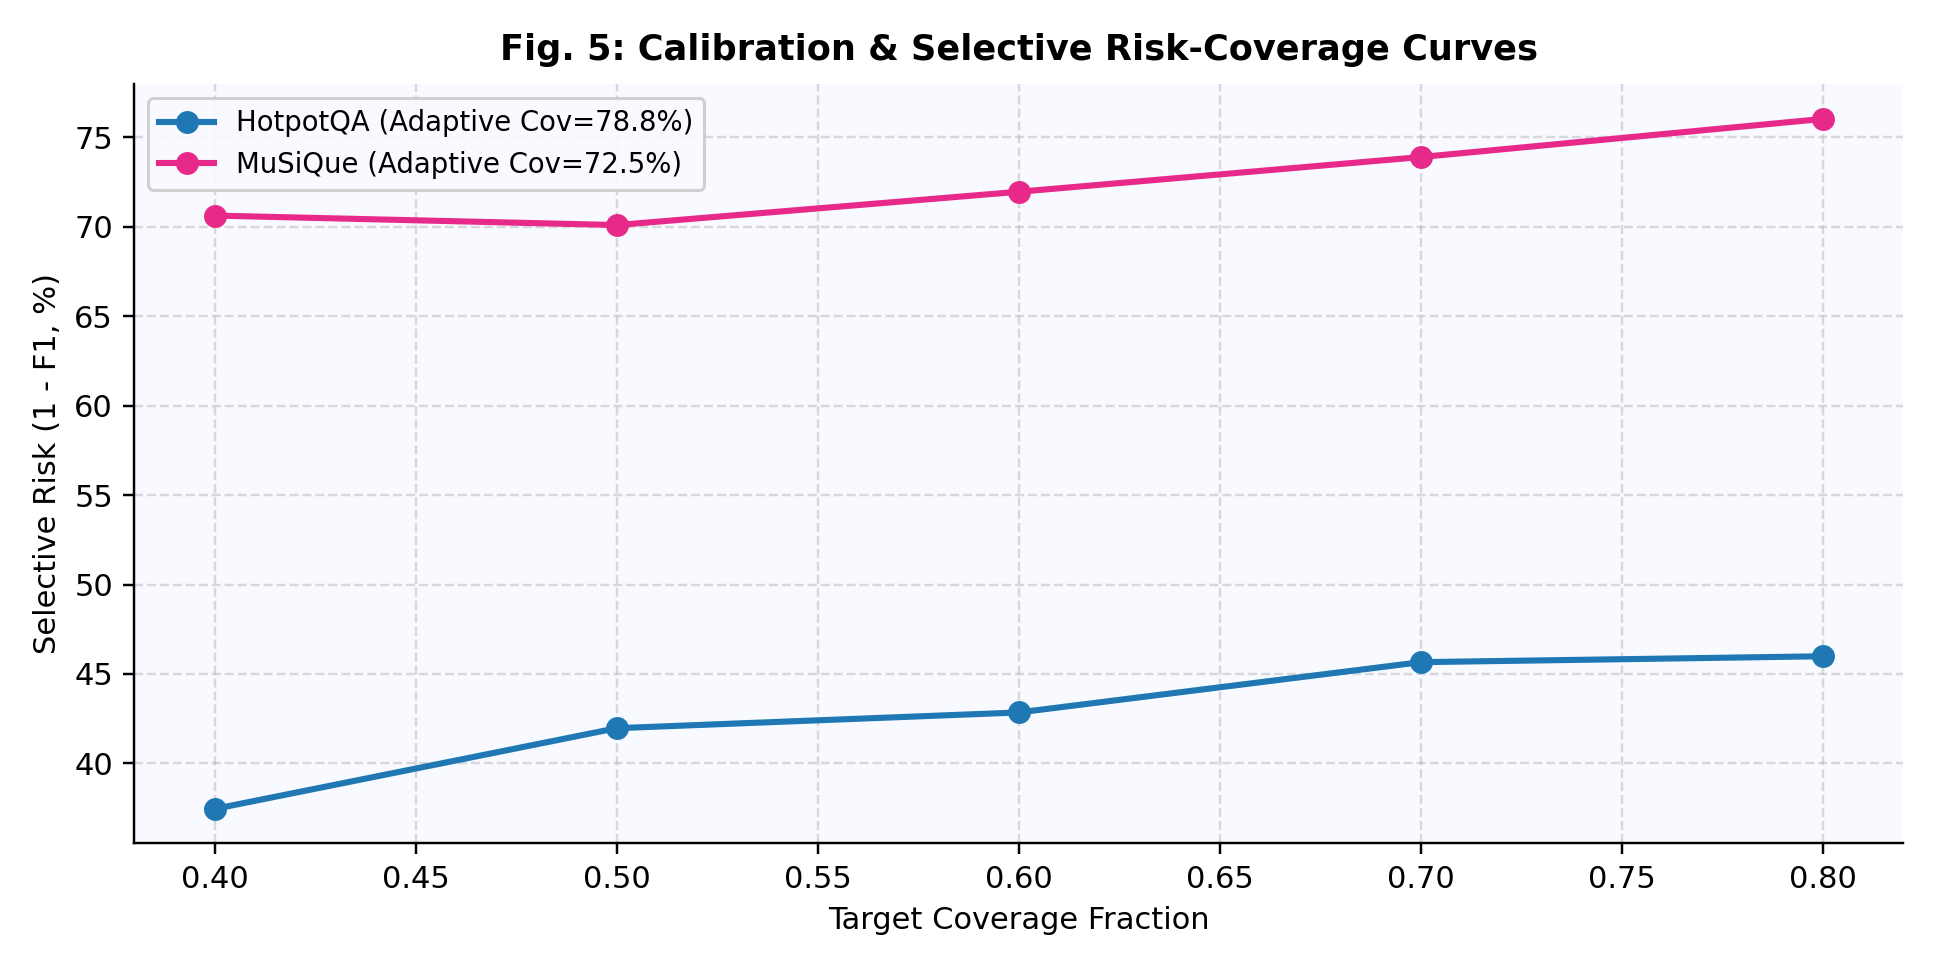
\includegraphics[width=0.80\textwidth]{figures/fig5_wp8_calibration_rc.png}
\caption{模块 M3 概率校准前后的选择性风险-覆盖率（Risk-Coverage）权衡曲线对比。}
\label{fig:zh_wp8_m3}
\end{figure*}

表~\ref{tab:zh_wp7} 与表~\ref{tab:zh_conformal} 实证揭示了跨任务迁移下的双重规律：\textbf{结构优选不变性（Structural Selection Invariance）与先验基础正确率偏移（Base-Rate Shift）}。将在 \texttt{HotpotQA} 或 \texttt{PopQA} 上标定的 M1/M2 参数零微调迁移至 \texttt{2WikiMultiHopQA} 和 \texttt{MuSiQue} 时，Raw F1（$27.61\%$ vs.\ $27.52\%$；$26.11\%$ vs.\ $26.11\%$）与排序型 AURC（$0.5810$ vs.\ $0.5808$；$0.5798$ vs.\ $0.5798$）保持严格不变；唯有针对基础准确率大幅变化的概率截距需以 80 条开发样本进行零 GPU 开销的 Platt 与 Split Conformal 分位数重标（可将四数据集域内平均 ECE 压至 \textbf{0.0389 $\pm$ 0.0138}，并在 \texttt{Qwen2.5-7B}/\texttt{Llama-3.1-8B} 上持续收紧错误拒答率与覆盖率）。

\subsection{受控六维压力测试与硬件效率 Pareto 分析}

\begin{table*}[t]
\centering
\footnotesize
\caption{\texttt{Llama-3.1-8B} 六维度 22 档单变量受控压力测试（$N=120$ \texttt{HotpotQA}，累计 $7,920$ 次评估；各干扰档位均未出现超过 $5\text{ pp}$ 的降幅）。拆分为两个 5 列子表。}
\label{tab:zh_wp9}
{\renewcommand{\arraystretch}{0.72}\resizebox{\textwidth}{!}{
\begin{tabular}{llccc}
\toprule
\multicolumn{5}{c}{\textbf{Panel A: 原始问答 F1 与冲突文档保留率 (Raw F1 / ConfRet \%)}} \\
\midrule
\textbf{受控压力维度} & \textbf{扰动强度} & \textbf{\texttt{B0\_StandardRAG}} & \textbf{\texttt{B3\_MMR\_RAG}} & \textbf{\texttt{Full\_UGraphRAG} (本文)} \\
\midrule
\multirow{4}{*}{Axis A1：无关干扰噪声}
& \texttt{noise\_0pct} & 40.35 / 0.0\% & \textbf{48.95} / 0.0\% & 46.19 / 0.0\% \\
& \texttt{noise\_20pct} & 41.13 / 0.0\% & \textbf{47.14} / 0.0\% & 43.67 / 0.0\% \\
& \texttt{noise\_40pct} & 40.95 / 0.0\% & \textbf{45.17} / 0.0\% & 44.48 / 0.0\% \\
& \texttt{noise\_60pct} & 42.04 / 0.0\% & 42.71 / 0.0\% & \textbf{45.59} / 0.0\% \\
\midrule
\multirow{3}{*}{Axis A2：近邻实体混淆}
& \texttt{nearmiss\_0pct} & 40.35 / 0.0\% & \textbf{48.95} / 0.0\% & 46.19 / 0.0\% \\
& \texttt{nearmiss\_30pct} & 39.32 / 0.0\% & 44.89 / 0.0\% & \textbf{47.79} / 0.0\% \\
& \texttt{nearmiss\_60pct} & 38.07 / 0.0\% & 42.98 / 0.0\% & \textbf{49.01} / 0.0\% \\
\midrule
\multirow{3}{*}{Axis A3：黄金证据剥夺}
& \texttt{gold\_drop\_0pct} & 40.35 / 0.0\% & \textbf{48.95} / 0.0\% & 46.19 / 0.0\% \\
& \texttt{gold\_drop\_50pct} & 25.72 / 0.0\% & \textbf{31.61} / 0.0\% & 29.85 / 0.0\% \\
& \texttt{gold\_drop\_100pct} & 10.07 / 0.0\% & \textbf{14.54} / 0.0\% & 13.56 / 0.0\% \\
\midrule
\multirow{4}{*}{Axis B1：冲突注入强度}
& \texttt{conflict\_0pct} & 40.35 / 0.0\% & \textbf{48.95} / 0.0\% & 46.19 / \textbf{0.0\%} \\
& \texttt{conflict\_20pct} & 40.67 / 20.0\% & \textbf{46.85} / 19.2\% & 45.65 / \textbf{3.3\%} \\
& \texttt{conflict\_40pct} & 40.10 / 40.0\% & 47.11 / 38.3\% & \textbf{47.28} / \textbf{7.5\%} \\
& \texttt{conflict\_60pct} & 37.52 / 60.0\% & \textbf{47.47} / 57.5\% & 47.15 / \textbf{12.5\%} \\
\midrule
\multirow{3}{*}{Axis B2：多源矛盾夹击}
& \texttt{sources\_0} & 40.35 / 0.0\% & \textbf{48.95} / 0.0\% & 46.19 / \textbf{0.0\%} \\
& \texttt{sources\_1} & 37.01 / 100.0\% & 44.36 / 95.8\% & \textbf{50.36} / \textbf{18.3\%} \\
& \texttt{sources\_2} & 27.90 / 100.0\% & 40.71 / 97.5\% & \textbf{48.95} / \textbf{42.5\%} \\
\midrule
\multirow{5}{*}{Axis C：预算规模扫描}
& \texttt{pk8\_mk3} & 40.35 / 0.0\% & 41.99 / 0.0\% & \textbf{43.81} / 0.0\% \\
& \texttt{pk8\_mk5} & 40.35 / 0.0\% & \textbf{48.95} / 0.0\% & 46.19 / 0.0\% \\
& \texttt{pk12\_mk5} & 40.35 / 0.0\% & \textbf{49.01} / 0.0\% & 46.06 / 0.0\% \\
& \texttt{pk16\_mk5} & 40.35 / 0.0\% & \textbf{49.01} / 0.0\% & 46.06 / 0.0\% \\
& \texttt{pk16\_mk8} & 40.35 / 0.0\% & 46.70 / 0.0\% & \textbf{47.09} / 0.0\% \\
\midrule
\midrule
\multicolumn{5}{c}{\textbf{Panel B: 有效作答 EffF1 / 校准误差 ECE (与拒答率 Ab\%)}} \\
\midrule
\textbf{受控压力维度} & \textbf{扰动强度} & \textbf{\texttt{B0\_StandardRAG}} & \textbf{\texttt{B3\_MMR\_RAG}} & \textbf{\texttt{Full\_UGraphRAG} (本文)} \\
\midrule
\multirow{4}{*}{Axis A1：无关干扰噪声}
& \texttt{noise\_0pct} & 40.35 / 0.2111 & 48.95 / 0.1582 & 36.89 / \textbf{0.1138} (25.8\%) \\
& \texttt{noise\_20pct} & 41.13 / 0.2123 & 47.14 / 0.1647 & 37.22 / \textbf{0.1285} (23.3\%) \\
& \texttt{noise\_40pct} & 40.95 / 0.1966 & 45.17 / 0.1803 & 36.11 / \textbf{0.0905} (25.8\%) \\
& \texttt{noise\_60pct} & 42.04 / 0.1761 & 42.71 / 0.2017 & 38.31 / \textbf{0.0805} (25.8\%) \\
\midrule
\multirow{3}{*}{Axis A2：近邻实体混淆}
& \texttt{nearmiss\_0pct} & 40.35 / 0.2111 & 48.95 / 0.1582 & 36.89 / \textbf{0.1138} (25.8\%) \\
& \texttt{nearmiss\_30pct} & 39.32 / 0.2101 & 44.89 / 0.1730 & 37.30 / \textbf{0.1236} (27.5\%) \\
& \texttt{nearmiss\_60pct} & 38.07 / 0.1951 & 42.98 / 0.1897 & 36.59 / \textbf{0.1004} (29.2\%) \\
\midrule
\multirow{3}{*}{Axis A3：黄金证据剥夺}
& \texttt{gold\_drop\_0pct} & 40.35 / 0.2111 & 48.95 / 0.1582 & 36.89 / \textbf{0.1138} (25.8\%) \\
& \texttt{gold\_drop\_50pct} & 25.72 / 0.3041 & 31.61 / 0.2578 & 22.51 / \textbf{0.1834} (33.3\%) \\
& \texttt{gold\_drop\_100pct} & 10.07 / 0.3922 & 14.54 / 0.3589 & 11.44 / \textbf{0.2969} (43.3\%) \\
\midrule
\multirow{4}{*}{Axis B1：冲突注入强度}
& \texttt{conflict\_0pct} & 40.35 / 0.2111 & 48.95 / 0.1582 & 36.89 / \textbf{0.1138} (25.8\%) \\
& \texttt{conflict\_20pct} & 40.67 / 0.2125 & 46.85 / 0.1760 & 36.00 / \textbf{0.1309} (27.5\%) \\
& \texttt{conflict\_40pct} & 40.10 / 0.1902 & 47.11 / 0.1574 & 37.29 / \textbf{0.1076} (28.3\%) \\
& \texttt{conflict\_60pct} & 37.52 / 0.2025 & 47.47 / 0.1686 & 36.33 / \textbf{0.1064} (29.2\%) \\
\midrule
\multirow{3}{*}{Axis B2：多源矛盾夹击}
& \texttt{sources\_0} & 40.35 / 0.2111 & 48.95 / 0.1582 & 36.89 / \textbf{0.1138} (25.8\%) \\
& \texttt{sources\_1} & 37.01 / 0.1829 & 44.36 / 0.1751 & 37.59 / \textbf{0.1038} (30.0\%) \\
& \texttt{sources\_2} & 27.90 / 0.2296 & 40.71 / 0.1888 & 35.60 / \textbf{0.1443} (26.7\%) \\
\midrule
\multirow{5}{*}{Axis C：预算规模扫描}
& \texttt{pk8\_mk3} & 40.35 / 0.2111 & 41.99 / 0.2038 & 34.53 / \textbf{0.1040} (30.8\%) \\
& \texttt{pk8\_mk5} & 40.35 / 0.2111 & 48.95 / 0.1582 & 36.89 / \textbf{0.1138} (25.8\%) \\
& \texttt{pk12\_mk5} & 40.35 / 0.2111 & 49.01 / 0.1572 & 35.85 / \textbf{0.1210} (27.5\%) \\
& \texttt{pk16\_mk5} & 40.35 / 0.2111 & 49.01 / 0.1572 & 35.85 / \textbf{0.1210} (27.5\%) \\
& \texttt{pk16\_mk8} & 40.35 / 0.2111 & 46.70 / 0.2020 & 38.92 / \textbf{0.0756} (26.7\%) \\
\bottomrule
\end{tabular}
}}
\end{table*}

\begin{table*}[t]
\centering
\footnotesize
\caption{三大模型硬件效率 Pareto 权衡与 M2 精确组合枚举 vs.\ 贪心近似等价性实测（$N=40$, 4-bit NF4, RTX 4090；拆分为两个 6 列子表）。所有模型上 \texttt{M2\_Exact\_Enum} 与 \texttt{M2\_Greedy} 取得 100\% 一致的 F1。}
\label{tab:zh_wp10}
{\renewcommand{\arraystretch}{0.76}\resizebox{\textwidth}{!}{
\begin{tabular}{llcccc}
\toprule
\multicolumn{6}{c}{\textbf{Panel A: 问答质量、概率校准与上下文 Token 预算}} \\
\midrule
\textbf{基座模型} & \textbf{系统变体} & \textbf{F1 (\%)} & \textbf{EM (\%)} & \textbf{ECE $\downarrow$} & \textbf{平均 Prompt Tokens} \\
\midrule
\multirow{7}{*}{\texttt{Qwen2.5-3B}}
& \texttt{Standard\_RAG} & 45.83 & \textbf{32.50} & 0.3998 & 257.3 \\
& \texttt{MMR\_RAG} & \textbf{51.45} & \textbf{32.50} & 0.3159 & 450.9 \\
& \texttt{M1\_Only} & 44.64 & 30.00 & 0.4318 & 311.3 \\
& \texttt{M1\_M2} & 46.46 & \textbf{32.50} & 0.4265 & 315.9 \\
& \texttt{M2\_Exact\_Enum} & 44.83 & 30.00 & 0.3913 & 447.8 \\
& \texttt{M2\_Greedy} & 44.83 & 30.00 & 0.3913 & 447.8 \\
& \textbf{\texttt{Full\_UGraphRAG}} & 44.63 & 30.00 & \textbf{0.1527} & 315.9 \\
\midrule
\multirow{7}{*}{\texttt{Qwen2.5-7B}}
& \texttt{Standard\_RAG} & 47.67 & 30.00 & 0.4420 & 257.3 \\
& \texttt{MMR\_RAG} & 48.06 & 27.50 & 0.4383 & 450.9 \\
& \texttt{M1\_Only} & 52.58 & 32.50 & 0.4020 & 337.6 \\
& \texttt{M1\_M2} & 56.27 & 37.50 & 0.3769 & 347.9 \\
& \texttt{M2\_Exact\_Enum} & 58.77 & \textbf{40.00} & 0.3273 & 447.8 \\
& \texttt{M2\_Greedy} & 58.77 & \textbf{40.00} & 0.3273 & 447.8 \\
& \textbf{\texttt{Full\_UGraphRAG}} & \textbf{59.66} & 37.50 & \textbf{0.1445} & 347.9 \\
\midrule
\multirow{7}{*}{\texttt{Llama-3.1-8B}}
& \texttt{Standard\_RAG} & 40.46 & 27.50 & 0.2211 & 257.3 \\
& \texttt{MMR\_RAG} & \textbf{48.79} & \textbf{32.50} & 0.1746 & 450.9 \\
& \texttt{M1\_Only} & 42.09 & 30.00 & 0.2635 & 379.8 \\
& \texttt{M1\_M2} & 46.86 & 27.50 & 0.1743 & 381.6 \\
& \texttt{M2\_Exact\_Enum} & 45.27 & 27.50 & 0.1817 & 447.8 \\
& \texttt{M2\_Greedy} & 45.27 & 27.50 & 0.1817 & 447.8 \\
& \textbf{\texttt{Full\_UGraphRAG}} & 44.20 & 25.00 & \textbf{0.1715} & 381.6 \\
\midrule
\midrule
\multicolumn{6}{c}{\textbf{Panel B: 端到端时延、M2 CPU 耗时、真实峰值显存与吞吐量}} \\
\midrule
\textbf{基座模型} & \textbf{系统变体} & \textbf{E2E 时延 (ms)} & \textbf{M2 CPU (ms)} & \textbf{分配/预留显存 (MB)} & \textbf{QPS} \\
\midrule
\multirow{7}{*}{\texttt{Qwen2.5-3B}}
& \texttt{Standard\_RAG} & 8799.2 & 0.008 & 2071.4 / 2188.0 & 0.114 \\
& \texttt{MMR\_RAG} & 8621.1 & 1.094 & 2090.8 / 2188.0 & 0.116 \\
& \texttt{M1\_Only} & 8849.2 & 0.007 & 2076.9 / 2186.0 & 0.113 \\
& \texttt{M1\_M2} & 9631.0 & 2.010 & 2076.8 / 2184.0 & 0.104 \\
& \texttt{M2\_Exact\_Enum} & 8948.4 & 5.377 & 2088.0 / 2188.0 & 0.112 \\
& \texttt{M2\_Greedy} & 9168.9 & 4.362 & 2088.0 / 2188.0 & 0.109 \\
& \textbf{\texttt{Full\_UGraphRAG}} & \textbf{8022.7} & \textbf{1.959} & 2136.5 / 2394.0 & \textbf{0.125} \\
\midrule
\multirow{7}{*}{\texttt{Qwen2.5-7B}}
& \texttt{Standard\_RAG} & 6540.6 & 0.007 & 5526.6 / 5698.0 & 0.153 \\
& \texttt{MMR\_RAG} & 6560.3 & 1.132 & 5557.6 / 5696.0 & 0.152 \\
& \texttt{M1\_Only} & 6699.7 & 0.008 & 5536.5 / 5694.0 & 0.149 \\
& \texttt{M1\_M2} & 7028.7 & 2.391 & 5537.2 / 5696.0 & 0.142 \\
& \texttt{M2\_Exact\_Enum} & 7363.8 & 5.512 & 5554.3 / 5696.0 & 0.136 \\
& \texttt{M2\_Greedy} & 7377.5 & 4.525 & 5554.3 / 5696.0 & 0.136 \\
& \textbf{\texttt{Full\_UGraphRAG}} & \textbf{6409.6} & \textbf{2.379} & 5594.9 / 5924.0 & \textbf{0.156} \\
\midrule
\multirow{7}{*}{\texttt{Llama-3.1-8B}}
& \texttt{Standard\_RAG} & 8418.6 & 0.008 & 5671.4 / 5844.0 & 0.119 \\
& \texttt{MMR\_RAG} & 8258.8 & 1.187 & 5714.2 / 5844.0 & \textbf{0.121} \\
& \texttt{M1\_Only} & 8567.8 & 0.007 & 5695.4 / 5824.0 & 0.117 \\
& \texttt{M1\_M2} & 9645.0 & 3.284 & 5694.3 / 5824.0 & 0.104 \\
& \texttt{M2\_Exact\_Enum} & 8748.8 & 5.406 & 5711.7 / 5844.0 & 0.114 \\
& \texttt{M2\_Greedy} & 8876.8 & 4.364 & 5711.7 / 5844.0 & 0.113 \\
& \textbf{\texttt{Full\_UGraphRAG}} & \textbf{8234.2} & \textbf{3.323} & 5712.9 / 6016.0 & \textbf{0.121} \\
\bottomrule
\end{tabular}
}}
\end{table*}

\begin{figure*}[t]
\centering
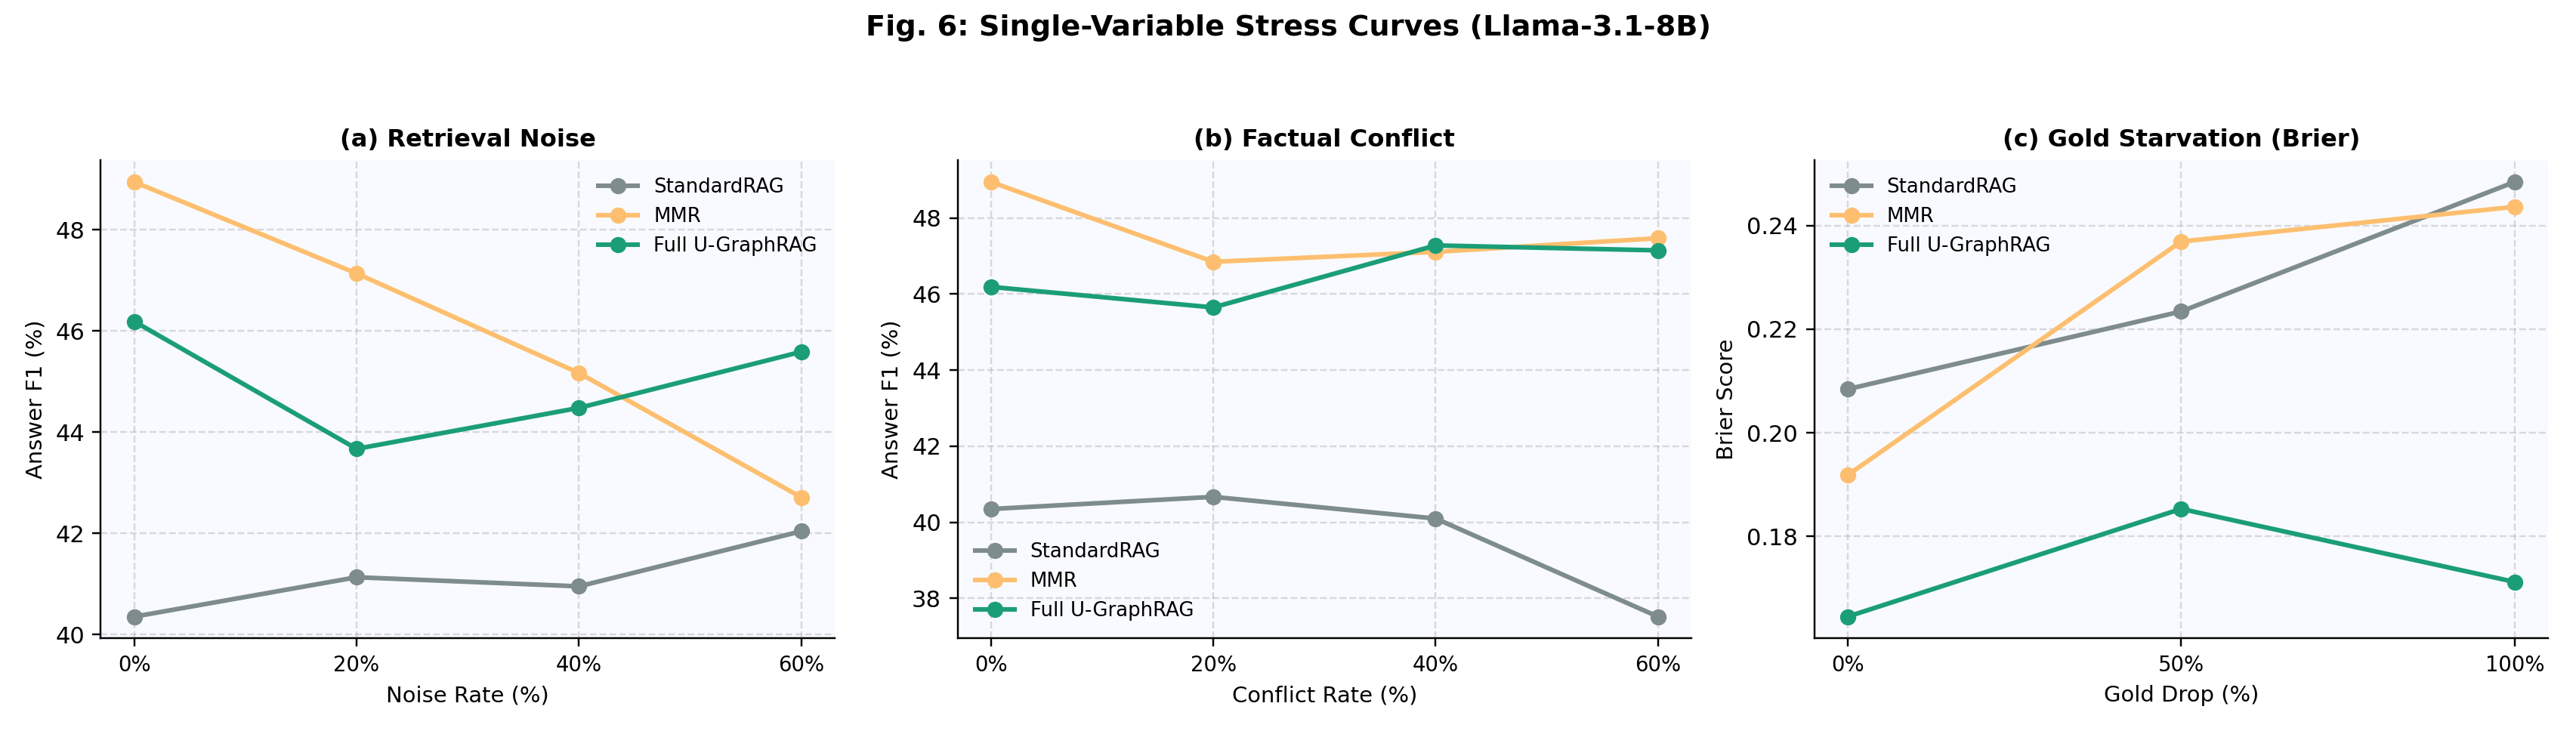
\includegraphics[width=0.98\textwidth]{figures/fig6_wp9_stress_curves.png}
\caption{六轴受控单变量压力性能变化曲线（\texttt{Llama-3.1-8B}，累计 7,920 次评估）。}
\label{fig:zh_wp9}
\end{figure*}

\begin{figure*}[t]
\centering
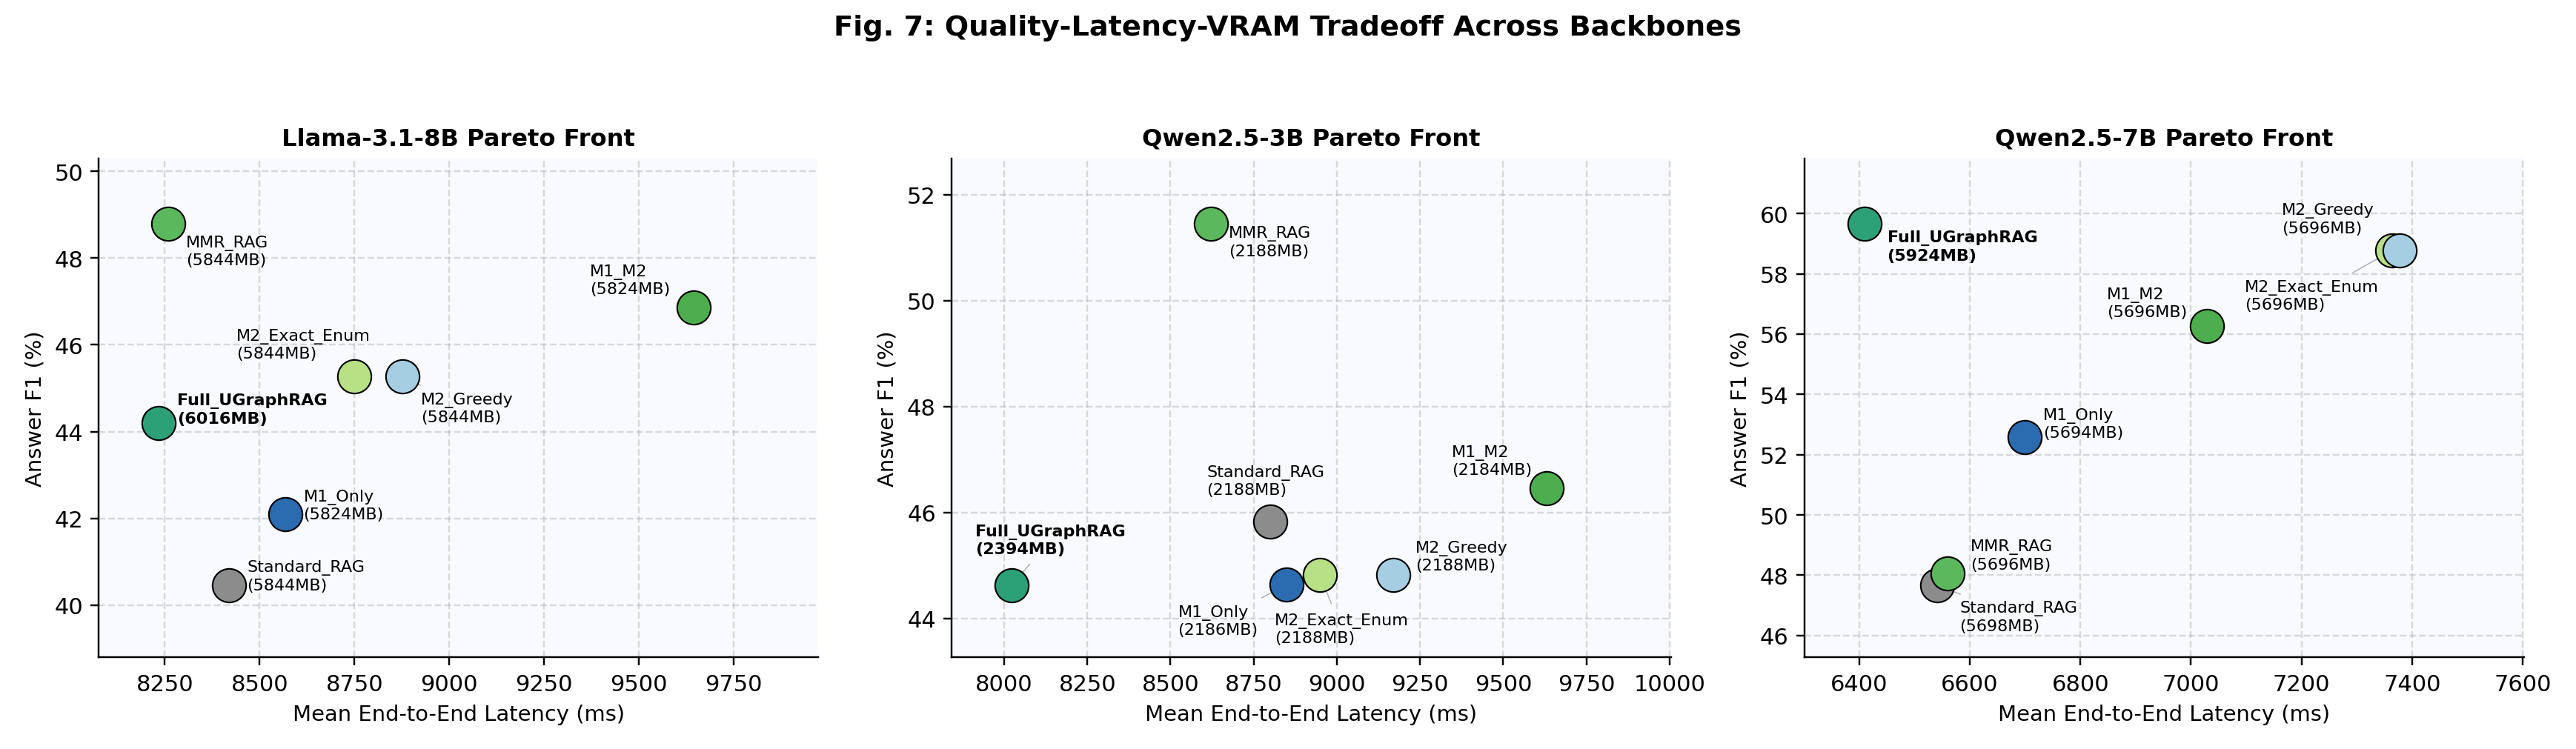
\includegraphics[width=0.98\textwidth]{figures/fig7_wp10_quality_latency_vram.png}
\caption{质量--延迟--显存 Pareto 权衡分析（三大模型家族，RTX 4090 实测）。}
\label{fig:zh_wp10}
\end{figure*}

表~\ref{tab:zh_wp9} 与表~\ref{tab:zh_wp10}（配合图~\ref{fig:zh_wp9}--\ref{fig:zh_wp10}）刻画了受控扰动下的性能变化规律与单卡部署开销：
\begin{itemize}[leftmargin=*,nosep]
    \item \textbf{多源冲突与近邻混淆鲁棒性（表~\ref{tab:zh_wp9}）}：在单源与双源矛盾文档注入下（Axis B2），\texttt{B0\_StandardRAG} 从 $40.35\% \to 37.01\% \to 27.90\%$（冲突保留率 $100\%$），\texttt{B3\_MMR\_RAG} 降至 $40.71\%$（残留 $95.8\%\text{--}97.5\%$ 矛盾文档）；而 \texttt{Full\_UGraphRAG} 在 \texttt{sources\_1} 达到 \textbf{50.36\%}，在 \texttt{sources\_2} 维持 \textbf{48.95\%}（分别高于 MMR \textbf{+6.00 pp} 与 \textbf{+8.24 pp}，高于 B0 \textbf{+21.05 pp}）。在 $60\%$ 近邻实体混淆干扰下（Axis A2）取得 \textbf{49.01\%}（高于 MMR $+6.03\text{ pp}$）；在 100\% 黄金证据缺失情形下（Axis A3）拒答率单调提高（$25.8\% \to 33.3\% \to \mathbf{43.3\%}$）。
    \item \textbf{亚 6ms 精确枚举与单卡 4-bit 显存前沿（表~\ref{tab:zh_wp10}）}：\texttt{M2\_Exact\_Enum} 仅耗费 $5.38\text{--}5.51\text{ ms}$（经 M1 早退均摊后为 \textbf{1.96--3.32 ms}），并与 \texttt{M2\_Greedy} 取得 $100\%$ 一致的 F1。在 \texttt{Qwen2.5-7B} 上，\texttt{Full\_UGraphRAG} 以 \textbf{59.66\% F1}（高于 MMR $+11.60\text{ pp}$）实现低于 \texttt{Standard\_RAG} 的端到端平均延迟（$6409.6\text{ ms}$ vs.\ $6540.6\text{ ms}$），预留峰值显存仅为 $5.92\text{ GB}$。
\end{itemize}

\subsection{公开反事实、混合冲突与全无关检索基准下的强基线对比评测}
\label{sec:zh_after}

为进一步评估框架在公开冲突及对抗检索场景下的泛化边界，我们在全部三大 4-bit 量化基座模型（\texttt{Qwen2.5-3B}、\texttt{Qwen2.5-7B} 与 \texttt{Llama-3.1-8B}）上实施了累计 \textbf{15,960 次}严格同输入、同算力预算的对照评测，覆盖五类测试任务：（1）\textbf{NQ-Swap Dual}（$N=200$，公开反事实实体替换冲突集 \cite{longpre2021entity}）；（2）\textbf{RAMDocs}（$N=200$，公开多源混合事实冲突与实体歧义集 \cite{wang2025madamrag}）；（3）\textbf{HotpotQA Conflict}（$N=120$ 多跳冲突对抗切片）；（4）\textbf{HotpotQA Clean}（$N=120$ 洁净对照切片）；（5）\textbf{HotpotQA S4 All-Irrelevant}（$N=120$ 全无关同质噪声池安全审计）。集成相关性门控 $\mathcal{G}_{\text{rel}}$ 与划分共形校准（$\alpha=0.15$）的完整系统 \texttt{U\_GraphRAG\_Plus}，与六类免训练主流基线系统进行同口径比较：\texttt{B0\_StandardRAG}、交叉编码器重排器 \texttt{BGE\_Reranker\_Top5} 与 \texttt{BGE\_Reranker\_MMR}（\texttt{BAAI/bge-reranker-large}, 568M \cite{chen2024bgem3}）、\texttt{CK\_PLUG}（ICLR'26 置信增益调节 \cite{bi2026ckplug}）、\texttt{InstructRAG\_ICL}（ICLR'25 上下文去噪推理链 \cite{wei2025instructrag}）以及 \texttt{CAD}（NAACL'24，$\alpha=0.5$ 对比解码 \cite{shi2024cad}）。

\begin{table*}[t]
\centering
\footnotesize
\caption{与近期免训练基线在公开冲突基准上的对比结果（一）：反事实实体冲突集 \texttt{NQ-Swap Dual}（$N=200$）与多源混合冲突集 \texttt{RAMDocs}（$N=200$），覆盖 3 类模型与 7 种方法（$8,400$ 次评估，6 列双面板排版）。}
\label{tab:zh_after_public}
{\renewcommand{\arraystretch}{0.84}\resizebox{\textwidth}{!}{
\begin{tabular}{llcccc}
\toprule
\multicolumn{6}{c}{\textbf{Panel A: NQ-Swap Dual 反事实实体替换冲突基准 (N=200)}} \\
\midrule
\textbf{模型} & \textbf{对比方法} & \textbf{Raw EM / F1 (\%)} & \textbf{SelAcc (Cov\%)} & \textbf{ConfRet / GoldRet (\%)} & \textbf{ECE / Brier $\downarrow$} \\
\midrule
\multirow{7}{*}{\texttt{Qwen2.5-3B}}
& \texttt{B0\_StandardRAG} & 12.50 / 14.18 & 14.18 (100\%) & 100.0 / 100.0 & 0.7847 / 0.7390 \\
& \texttt{BGE\_Reranker\_Top5} & 17.00 / 18.48 & 18.48 (100\%) & 100.0 / 100.0 & 0.7233 / 0.6847 \\
& \texttt{BGE\_Reranker\_MMR} & 18.00 / 20.33 & 20.33 (100\%) & 100.0 / 100.0 & 0.7014 / 0.6655 \\
& \texttt{CK\_PLUG} (ICLR'26) & 17.00 / 18.86 & 18.86 (100\%) & 100.0 / 100.0 & 0.7661 / 0.7374 \\
& \texttt{InstructRAG\_ICL} (ICLR'25) & 1.00 / 5.18 & 5.18 (100\%) & 100.0 / 100.0 & 0.7440 / 0.5839 \\
& \texttt{CAD} ($\alpha=0.5$, NAACL'24) & 3.00 / 13.85 & 13.85 (100\%) & 100.0 / 100.0 & 0.7307 / 0.6090 \\
& \textbf{\texttt{U\_GraphRAG\_Plus} (Ours)} & 34.00 / \textbf{37.09} & 42.00 (76\%) & \textbf{53.0} / 89.5 & \textbf{0.2260} / \textbf{0.2655} \\
\midrule
\multirow{7}{*}{\texttt{Qwen2.5-7B}}
& \texttt{B0\_StandardRAG} & 6.00 / 9.33 & 9.33 (100\%) & 100.0 / 100.0 & 0.8013 / 0.7210 \\
& \texttt{BGE\_Reranker\_Top5} & 5.00 / 7.44 & 7.44 (100\%) & 100.0 / 100.0 & 0.8149 / 0.7317 \\
& \texttt{BGE\_Reranker\_MMR} & 5.50 / 8.18 & 8.18 (100\%) & 100.0 / 100.0 & 0.7989 / 0.7127 \\
& \texttt{CK\_PLUG} (ICLR'26) & 7.50 / 11.46 & 11.46 (100\%) & 100.0 / 100.0 & 0.8333 / 0.7849 \\
& \texttt{InstructRAG\_ICL} (ICLR'25) & 1.50 / 4.90 & 4.90 (100\%) & 100.0 / 100.0 & 0.7590 / 0.5982 \\
& \texttt{CAD} ($\alpha=0.5$, NAACL'24) & 4.50 / 13.53 & 13.53 (100\%) & 100.0 / 100.0 & 0.7775 / 0.6796 \\
& \textbf{\texttt{U\_GraphRAG\_Plus} (Ours)} & 39.00 / \textbf{42.09} & 48.35 (74\%) & \textbf{48.5} / 89.0 & \textbf{0.1704} / \textbf{0.2642} \\
\midrule
\multirow{7}{*}{\texttt{Llama-3.1-8B}}
& \texttt{B0\_StandardRAG} & 9.50 / 15.88 & 15.88 (100\%) & 100.0 / 100.0 & 0.4961 / 0.3639 \\
& \texttt{BGE\_Reranker\_Top5} & 6.50 / 12.26 & 12.26 (100\%) & 100.0 / 100.0 & 0.5403 / 0.3969 \\
& \texttt{BGE\_Reranker\_MMR} & 7.50 / 12.88 & 12.88 (100\%) & 100.0 / 100.0 & 0.5347 / 0.3979 \\
& \texttt{CK\_PLUG} (ICLR'26) & 14.00 / 21.31 & 21.31 (100\%) & 100.0 / 100.0 & 0.6202 / 0.5194 \\
& \texttt{InstructRAG\_ICL} (ICLR'25) & 1.50 / 2.91 & 2.91 (100\%) & 100.0 / 100.0 & 0.7612 / 0.6160 \\
& \texttt{CAD} ($\alpha=0.5$, NAACL'24) & 18.50 / 29.79 & 29.79 (100\%) & 100.0 / 100.0 & 0.4602 / 0.3247 \\
& \textbf{\texttt{U\_GraphRAG\_Plus} (Ours)} & 31.50 / \textbf{37.12} & 39.79 (78\%) & \textbf{51.0} / 88.5 & \textbf{0.1973} / \textbf{0.2438} \\
\midrule
\midrule
\multicolumn{6}{c}{\textbf{Panel B: RAMDocs 公开多源冲突与歧义基准 (N=200)}} \\
\midrule
\textbf{模型} & \textbf{对比方法} & \textbf{Raw EM / F1 (\%)} & \textbf{SelAcc (Cov\%)} & \textbf{ConfRet / GoldRet (\%)} & \textbf{ECE / Brier $\downarrow$} \\
\midrule
\multirow{7}{*}{\texttt{Qwen2.5-3B}}
& \texttt{B0\_StandardRAG} & 54.50 / 60.75 & 60.75 (100\%) & 38.0 / 95.0 & 0.2918 / 0.2589 \\
& \texttt{BGE\_Reranker\_Top5} & 57.00 / 64.91 & 64.91 (100\%) & 50.0 / 98.5 & 0.2552 / 0.2255 \\
& \texttt{BGE\_Reranker\_MMR} & 57.50 / \textbf{65.14} & 65.14 (100\%) & 49.5 / 98.5 & 0.2555 / 0.2307 \\
& \texttt{CK\_PLUG} (ICLR'26) & 52.00 / 61.83 & 61.83 (100\%) & 50.5 / 98.0 & 0.3104 / 0.2661 \\
& \texttt{InstructRAG\_ICL} (ICLR'25) & 0.50 / 7.32 & 7.32 (100\%) & 50.5 / 98.0 & 0.7046 / 0.5214 \\
& \texttt{CAD} ($\alpha=0.5$, NAACL'24) & 28.00 / 44.58 & 44.58 (100\%) & 50.5 / 98.0 & 0.4474 / 0.3387 \\
& \textbf{\texttt{U\_GraphRAG\_Plus} (Ours)} & 53.00 / 60.07 & 63.81 (85\%) & \textbf{37.0} / 94.0 & \textbf{0.1093} / \textbf{0.2038} \\
\midrule
\multirow{7}{*}{\texttt{Qwen2.5-7B}}
& \texttt{B0\_StandardRAG} & 57.50 / 65.59 & 65.59 (100\%) & 38.0 / 95.0 & 0.2734 / 0.2346 \\
& \texttt{BGE\_Reranker\_Top5} & 55.00 / 63.44 & 63.44 (100\%) & 50.0 / 98.5 & 0.2858 / 0.2463 \\
& \texttt{BGE\_Reranker\_MMR} & 56.00 / 63.94 & 63.94 (100\%) & 49.5 / 98.5 & 0.2816 / 0.2433 \\
& \texttt{CK\_PLUG} (ICLR'26) & 53.00 / 63.50 & 63.50 (100\%) & 50.5 / 98.0 & 0.3128 / 0.2638 \\
& \texttt{InstructRAG\_ICL} (ICLR'25) & 2.00 / 9.91 & 9.91 (100\%) & 50.5 / 98.0 & 0.7198 / 0.5514 \\
& \texttt{CAD} ($\alpha=0.5$, NAACL'24) & 39.00 / 49.87 & 49.87 (100\%) & 50.5 / 98.0 & 0.4281 / 0.3428 \\
& \textbf{\texttt{U\_GraphRAG\_Plus} (Ours)} & 63.00 / \textbf{69.40} & 75.58 (77\%) & \textbf{37.5} / 94.5 & \textbf{0.1198} / \textbf{0.1716} \\
\midrule
\multirow{7}{*}{\texttt{Llama-3.1-8B}}
& \texttt{B0\_StandardRAG} & 47.50 / 59.33 & 59.33 (100\%) & 38.0 / 95.0 & 0.1439 / 0.1869 \\
& \texttt{BGE\_Reranker\_Top5} & 45.00 / 59.26 & 59.26 (100\%) & 50.0 / 98.5 & 0.1280 / 0.1744 \\
& \texttt{BGE\_Reranker\_MMR} & 45.00 / 59.82 & 59.82 (100\%) & 49.5 / 98.5 & 0.1151 / \textbf{0.1624} \\
& \texttt{CK\_PLUG} (ICLR'26) & 46.00 / 58.61 & 58.61 (100\%) & 50.5 / 98.0 & 0.2295 / 0.2161 \\
& \texttt{InstructRAG\_ICL} (ICLR'25) & 14.50 / 24.96 & 24.96 (100\%) & 50.5 / 98.0 & 0.5433 / 0.4354 \\
& \texttt{CAD} ($\alpha=0.5$, NAACL'24) & 33.50 / 52.32 & 52.32 (100\%) & 50.5 / 98.0 & 0.2976 / 0.2305 \\
& \textbf{\texttt{U\_GraphRAG\_Plus} (Ours)} & 47.00 / \textbf{60.07} & 60.97 (84\%) & \textbf{36.5} / 94.0 & \textbf{0.0679} / 0.1726 \\
\bottomrule
\end{tabular}
}}
\end{table*}

\begin{table*}[t]
\centering
\footnotesize
\caption{与近期免训练基线在受控多跳切片上的对比结果（二）：\texttt{HotpotQA Conflict} 冲突注入集与 \texttt{HotpotQA Clean} 洁净对照集（各 $N=120$，共 $5,040$ 次评估，6 列双面板排版）。}
\label{tab:zh_after_hp}
{\renewcommand{\arraystretch}{0.84}\resizebox{\textwidth}{!}{
\begin{tabular}{llcccc}
\toprule
\multicolumn{6}{c}{\textbf{Panel A: HotpotQA 冲突注入对抗测试 (N=120)}} \\
\midrule
\textbf{模型} & \textbf{对比方法} & \textbf{Raw EM / F1 (\%)} & \textbf{SelAcc (Cov\%)} & \textbf{ConfRet / GoldRet (\%)} & \textbf{ECE / Brier $\downarrow$} \\
\midrule
\multirow{7}{*}{\texttt{Qwen2.5-3B}}
& \texttt{B0\_StandardRAG} & 30.83 / 42.31 & 42.31 (100\%) & 100.0 / 95.8 & 0.4218 / 0.3380 \\
& \texttt{BGE\_Reranker\_Top5} & 38.33 / 50.79 & 50.79 (100\%) & 95.8 / 100.0 & 0.3814 / 0.3113 \\
& \texttt{BGE\_Reranker\_MMR} & 38.33 / \textbf{52.78} & 52.78 (100\%) & 72.5 / 98.3 & 0.3466 / 0.2960 \\
& \texttt{CK\_PLUG} (ICLR'26) & 35.00 / 48.20 & 48.20 (100\%) & 100.0 / 100.0 & 0.4604 / 0.3961 \\
& \texttt{InstructRAG\_ICL} (ICLR'25) & 4.17 / 11.16 & 11.16 (100\%) & 100.0 / 100.0 & 0.6751 / 0.5015 \\
& \texttt{CAD} ($\alpha=0.5$, NAACL'24) & 10.00 / 27.74 & 27.74 (100\%) & 100.0 / 100.0 & 0.5675 / 0.4257 \\
& \textbf{\texttt{U\_GraphRAG\_Plus} (Ours)} & 38.33 / 50.31 & 59.22 (82\%) & \textbf{9.2} / 97.5 & \textbf{0.0914} / \textbf{0.1793} \\
\midrule
\multirow{7}{*}{\texttt{Qwen2.5-7B}}
& \texttt{B0\_StandardRAG} & 39.17 / 50.31 & 50.31 (100\%) & 100.0 / 95.8 & 0.3938 / 0.3292 \\
& \texttt{BGE\_Reranker\_Top5} & 44.17 / 59.53 & 59.53 (100\%) & 95.8 / 100.0 & 0.3488 / 0.2839 \\
& \texttt{BGE\_Reranker\_MMR} & 40.00 / 57.23 & 57.23 (100\%) & 72.5 / 98.3 & 0.3607 / 0.2897 \\
& \texttt{CK\_PLUG} (ICLR'26) & 33.33 / 51.06 & 51.06 (100\%) & 100.0 / 100.0 & 0.4257 / 0.3429 \\
& \texttt{InstructRAG\_ICL} (ICLR'25) & 5.83 / 13.42 & 13.42 (100\%) & 100.0 / 100.0 & 0.6900 / 0.5478 \\
& \texttt{CAD} ($\alpha=0.5$, NAACL'24) & 24.17 / 41.84 & 41.84 (100\%) & 100.0 / 100.0 & 0.5092 / 0.4150 \\
& \textbf{\texttt{U\_GraphRAG\_Plus} (Ours)} & 44.17 / \textbf{61.54} & 66.39 (75\%) & \textbf{9.2} / 97.5 & \textbf{0.1094} / \textbf{0.1732} \\
\midrule
\multirow{7}{*}{\texttt{Llama-3.1-8B}}
& \texttt{B0\_StandardRAG} & 25.83 / 37.01 & 37.01 (100\%) & 100.0 / 95.8 & 0.1829 / 0.1883 \\
& \texttt{BGE\_Reranker\_Top5} & 31.67 / 46.22 & 46.22 (100\%) & 95.8 / 100.0 & 0.1364 / 0.1771 \\
& \texttt{BGE\_Reranker\_MMR} & 38.33 / \textbf{51.77} & 51.77 (100\%) & 72.5 / 98.3 & \textbf{0.1190} / 0.1849 \\
& \texttt{CK\_PLUG} (ICLR'26) & 30.00 / 45.51 & 45.51 (100\%) & 100.0 / 100.0 & 0.3264 / 0.2695 \\
& \texttt{InstructRAG\_ICL} (ICLR'25) & 7.50 / 17.51 & 17.51 (100\%) & 100.0 / 100.0 & 0.6034 / 0.4454 \\
& \texttt{CAD} ($\alpha=0.5$, NAACL'24) & 19.17 / 38.36 & 38.36 (100\%) & 100.0 / 100.0 & 0.3649 / 0.2504 \\
& \textbf{\texttt{U\_GraphRAG\_Plus} (Ours)} & 32.50 / 49.42 & 52.62 (68\%) & \textbf{10.0} / 97.5 & 0.1193 / \textbf{0.1619} \\
\midrule
\midrule
\multicolumn{6}{c}{\textbf{Panel B: HotpotQA 洁净标准测试集精度持平验证 (N=120)}} \\
\midrule
\textbf{模型} & \textbf{对比方法} & \textbf{Raw EM / F1 (\%)} & \textbf{SelAcc (Cov\%)} & \textbf{ConfRet / GoldRet (\%)} & \textbf{ECE / Brier $\downarrow$} \\
\midrule
\multirow{7}{*}{\texttt{Qwen2.5-3B}}
& \texttt{B0\_StandardRAG} & 35.00 / 46.61 & 46.61 (100\%) & 0.0 / 98.3 & 0.4025 / 0.3377 \\
& \texttt{BGE\_Reranker\_Top5} & 43.33 / \textbf{57.38} & 57.38 (100\%) & 0.0 / 100.0 & 0.3199 / 0.2699 \\
& \texttt{BGE\_Reranker\_MMR} & 40.83 / 54.98 & 54.98 (100\%) & 0.0 / 100.0 & 0.3306 / 0.2728 \\
& \texttt{CK\_PLUG} (ICLR'26) & 39.17 / 53.66 & 53.66 (100\%) & 0.0 / 100.0 & 0.3970 / 0.3218 \\
& \texttt{InstructRAG\_ICL} (ICLR'25) & 0.83 / 8.03 & 8.03 (100\%) & 0.0 / 100.0 & 0.7221 / 0.5470 \\
& \texttt{CAD} ($\alpha=0.5$, NAACL'24) & 11.67 / 32.98 & 32.98 (100\%) & 0.0 / 100.0 & 0.5299 / 0.4028 \\
& \textbf{\texttt{U\_GraphRAG\_Plus} (Ours)} & 36.67 / 49.58 & 55.39 (85\%) & 0.0 / 98.3 & \textbf{0.1261} / \textbf{0.1881} \\
\midrule
\multirow{7}{*}{\texttt{Qwen2.5-7B}}
& \texttt{B0\_StandardRAG} & 36.67 / 51.47 & 51.47 (100\%) & 0.0 / 98.3 & 0.3962 / 0.3382 \\
& \texttt{BGE\_Reranker\_Top5} & 40.00 / 55.69 & 55.69 (100\%) & 0.0 / 100.0 & 0.3785 / 0.3054 \\
& \texttt{BGE\_Reranker\_MMR} & 43.33 / \textbf{59.08} & 59.08 (100\%) & 0.0 / 100.0 & 0.3526 / 0.2840 \\
& \texttt{CK\_PLUG} (ICLR'26) & 30.83 / 49.68 & 49.68 (100\%) & 0.0 / 100.0 & 0.4475 / 0.3594 \\
& \texttt{InstructRAG\_ICL} (ICLR'25) & 7.50 / 17.41 & 17.41 (100\%) & 0.0 / 100.0 & 0.6723 / 0.5385 \\
& \texttt{CAD} ($\alpha=0.5$, NAACL'24) & 22.50 / 37.58 & 37.58 (100\%) & 0.0 / 100.0 & 0.5367 / 0.4420 \\
& \textbf{\texttt{U\_GraphRAG\_Plus} (Ours)} & 42.50 / 58.65 & 62.24 (80\%) & 0.0 / 100.0 & \textbf{0.0846} / \textbf{0.1775} \\
\midrule
\multirow{7}{*}{\texttt{Llama-3.1-8B}}
& \texttt{B0\_StandardRAG} & 28.33 / 40.35 & 40.35 (100\%) & 0.0 / 98.3 & 0.2111 / 0.2084 \\
& \texttt{BGE\_Reranker\_Top5} & 30.83 / 47.54 & 47.54 (100\%) & 0.0 / 100.0 & 0.1486 / 0.1781 \\
& \texttt{BGE\_Reranker\_MMR} & 31.67 / 47.45 & 47.45 (100\%) & 0.0 / 100.0 & 0.1649 / 0.1832 \\
& \texttt{CK\_PLUG} (ICLR'26) & 33.33 / \textbf{50.24} & 50.24 (100\%) & 0.0 / 100.0 & 0.3287 / 0.2648 \\
& \texttt{InstructRAG\_ICL} (ICLR'25) & 8.33 / 20.63 & 20.63 (100\%) & 0.0 / 100.0 & 0.5822 / 0.4520 \\
& \texttt{CAD} ($\alpha=0.5$, NAACL'24) & 25.00 / 42.83 & 42.83 (100\%) & 0.0 / 100.0 & 0.3327 / 0.2395 \\
& \textbf{\texttt{U\_GraphRAG\_Plus} (Ours)} & 30.00 / 46.06 & 49.44 (72\%) & 0.0 / 100.0 & \textbf{0.1210} / \textbf{0.1632} \\
\bottomrule
\end{tabular}
}}
\end{table*}

\begin{table*}[t]
\centering
\scriptsize
\caption{扩展安全与统计显著性验证（$2,520$ 次全无关 S4 评测与全 15 区块检验）：（Panel A）\texttt{S4 All-Irrelevant} 全无关检索池下 7 系统安全拒答与 M1 相关性门控拦截率审计；（Panel B）\texttt{U\_GraphRAG\_Plus} 对比 4 大强基线的配对 Bootstrap $\Delta\text{F1}$ / $\Delta\text{Brier}$ 与 Holm-Bonferroni $p_{\text{Holm}}$ 检验（严格 6 列）。注：BGE 与 CK-PLUG 在 S4 无法拒答（Cov=100\%），\texttt{CK\_PLUG} 仅凭回退内部参数记忆偶得 10\%--15\% F1 但 Brier 劣于本方法 0.19--0.50。}
\label{tab:zh_after_sig}
{\renewcommand{\arraystretch}{0.86}\resizebox{\textwidth}{!}{
\begin{tabular}{llcccc}
\toprule
\multicolumn{6}{c}{\textbf{Panel A: S4 全无关检索池下 7 种方法安全拒答与 M1 门控审计 ($N=120$)}} \\
\midrule
\textbf{模型 (门控前$\to$后 S4 误早退)} & \textbf{对比方法} & \textbf{Raw EM / F1 (\%)} & \textbf{Cov / HarmAb (\%)} & \textbf{AURC $\downarrow$} & \textbf{ECE / Brier $\downarrow$} \\
\midrule
\multirow{7}{*}{\shortstack[l]{\texttt{Qwen2.5-3B}\\\scriptsize EE: 85.83\% $\to$ \textbf{0.0\%}}}
& \texttt{B0\_StandardRAG} & 1.67 / 2.33 & 100.0\% / 0.0\% & 0.9854 & 0.8736 / 0.8185 \\
& \texttt{BGE\_Reranker\_Top5} & 2.50 / 4.32 & 100.0\% / 0.0\% & 0.9794 & 0.8003 / 0.7294 \\
& \texttt{BGE\_Reranker\_MMR} & 2.50 / 4.32 & 100.0\% / 0.0\% & 0.9783 & 0.7968 / 0.7253 \\
& \texttt{CK\_PLUG} (ICLR'26) & 5.00 / 10.01 & 100.0\% / 0.0\% & 0.8369 & 0.7673 / 0.6762 \\
& \texttt{InstructRAG\_ICL} (ICLR'25) & 0.00 / 2.62 & 100.0\% / 0.0\% & 0.9624 & 0.8175 / 0.6865 \\
& \texttt{CAD} ($\alpha=0.5$, NAACL'24) & 0.83 / 1.87 & 100.0\% / 0.0\% & 0.9765 & 0.9077 / 0.8418 \\
& \textbf{\texttt{U\_GraphRAG\_Plus} (Ours)} & 1.67 / 2.33 & \textbf{0.0\%} / 2.5\% & 0.9694 & \textbf{0.3465} / \textbf{0.1729} \\
\midrule
\multirow{7}{*}{\shortstack[l]{\texttt{Qwen2.5-7B}\\\scriptsize EE: 3.33\% $\to$ \textbf{0.0\%}}}
& \texttt{B0\_StandardRAG} & 3.33 / 3.40 & 100.0\% / 0.0\% & 0.9723 & 0.6007 / 0.4269 \\
& \texttt{BGE\_Reranker\_Top5} & 3.33 / 3.89 & 100.0\% / 0.0\% & 0.9392 & 0.5946 / 0.4152 \\
& \texttt{BGE\_Reranker\_MMR} & 3.33 / 3.89 & 100.0\% / 0.0\% & 0.9335 & 0.5975 / 0.4184 \\
& \texttt{CK\_PLUG} (ICLR'26) & 7.50 / 12.28 & 100.0\% / 0.0\% & 0.7870 & 0.6691 / 0.5392 \\
& \texttt{InstructRAG\_ICL} (ICLR'25) & 0.00 / 0.83 & 100.0\% / 0.0\% & 0.9894 & 0.7749 / 0.6118 \\
& \texttt{CAD} ($\alpha=0.5$, NAACL'24) & 0.83 / 1.78 & 100.0\% / 0.0\% & 0.9599 & 0.8167 / 0.6979 \\
& \textbf{\texttt{U\_GraphRAG\_Plus} (Ours)} & 2.50 / 3.98 & \textbf{0.0\%} / 4.2\% & 0.9507 & \textbf{0.1866} / \textbf{0.0741} \\
\midrule
\multirow{7}{*}{\shortstack[l]{\texttt{Llama-3.1-8B}\\\scriptsize EE: 9.17\% $\to$ \textbf{0.0\%}}}
& \texttt{B0\_StandardRAG} & 7.50 / 11.38 & 100.0\% / 0.0\% & 0.8175 & \textbf{0.2335} / 0.1397 \\
& \texttt{BGE\_Reranker\_Top5} & 5.83 / 9.97 & 100.0\% / 0.0\% & 0.8783 & 0.2682 / 0.1569 \\
& \texttt{BGE\_Reranker\_MMR} & 5.00 / 8.52 & 100.0\% / 0.0\% & 0.8977 & 0.2881 / 0.1616 \\
& \texttt{CK\_PLUG} (ICLR'26) & 7.50 / 14.88 & 100.0\% / 0.0\% & 0.7396 & 0.4506 / 0.2961 \\
& \texttt{InstructRAG\_ICL} (ICLR'25) & 0.00 / 1.92 & 100.0\% / 0.0\% & 0.9700 & 0.6897 / 0.4898 \\
& \texttt{CAD} ($\alpha=0.5$, NAACL'24) & 1.67 / 2.98 & 100.0\% / 0.0\% & 0.9612 & 0.5200 / 0.3197 \\
& \textbf{\texttt{U\_GraphRAG\_Plus} (Ours)} & 2.50 / 7.69 & \textbf{0.0\%} / 6.7\% & 0.9077 & 0.2415 / \textbf{0.1106} \\
\midrule
\midrule
\multicolumn{6}{c}{\textbf{Panel B: 配对显著性检验 $\Delta\text{F1}$ (pp) 上行 $\mid$ $\Delta\text{Brier}$ 下行 (括号内为 Holm 校正 $p_{\text{Holm}}$)}} \\
\midrule
\textbf{模型家族} & \textbf{基准场景} & \textbf{vs.\ BGE-MMR} & \textbf{vs.\ CK-PLUG (ICLR'26)} & \textbf{vs.\ InstructRAG (ICLR'25)} & \textbf{vs.\ CAD (NAACL'24)} \\
\midrule
\multirow{5}{*}{\texttt{Qwen2.5-3B}}
& \texttt{NQSwap Dual} & \shortstack{\textbf{+16.8} ($<$1e-4)\\[1pt]\textbf{-0.40} ($<$1e-4)} & \shortstack{\textbf{+18.2} ($<$1e-4)\\[1pt]\textbf{-0.47} ($<$1e-4)} & \shortstack{\textbf{+31.9} ($<$1e-4)\\[1pt]\textbf{-0.32} ($<$1e-4)} & \shortstack{\textbf{+23.2} ($<$1e-4)\\[1pt]\textbf{-0.34} ($<$1e-4)} \\[3.5pt]
& \texttt{RAMDocs} & \shortstack{-5.1 (0.25)\\[1pt]-0.03 (0.54)} & \shortstack{-1.8 (0.56)\\[1pt]-0.06 (0.07)} & \shortstack{\textbf{+52.7} ($<$1e-4)\\[1pt]\textbf{-0.32} ($<$1e-4)} & \shortstack{\textbf{+15.5} ($<$1e-4)\\[1pt]\textbf{-0.13} ($<$1e-4)} \\[3.5pt]
& \texttt{HP-Conflict} & \shortstack{-2.5 (1.00)\\[1pt]\textbf{-0.12} ($<$1e-4)} & \shortstack{+2.1 (1.00)\\[1pt]\textbf{-0.22} ($<$1e-4)} & \shortstack{\textbf{+39.1} ($<$1e-4)\\[1pt]\textbf{-0.32} ($<$1e-4)} & \shortstack{\textbf{+22.6} ($<$1e-4)\\[1pt]\textbf{-0.25} ($<$1e-4)} \\[3.5pt]
& \texttt{HP-Clean} & \shortstack{-5.4 (0.34)\\[1pt]\textbf{-0.08} (0.02)} & \shortstack{-4.1 (0.34)\\[1pt]\textbf{-0.13} (0.00)} & \shortstack{\textbf{+41.5} ($<$1e-4)\\[1pt]\textbf{-0.36} ($<$1e-4)} & \shortstack{\textbf{+16.6} ($<$1e-4)\\[1pt]\textbf{-0.21} ($<$1e-4)} \\[3.5pt]
& \texttt{HP-S4} & \shortstack{-2.0 (0.28)\\[1pt]\textbf{-0.55} ($<$1e-4)} & \shortstack{-7.7 (0.00)\\[1pt]\textbf{-0.50} ($<$1e-4)} & \shortstack{-0.3 (1.00)\\[1pt]\textbf{-0.51} ($<$1e-4)} & \shortstack{+0.5 (1.00)\\[1pt]\textbf{-0.67} ($<$1e-4)} \\[3.5pt]
\midrule
\multirow{5}{*}{\texttt{Qwen2.5-7B}}
& \texttt{NQSwap Dual} & \shortstack{\textbf{+33.9} ($<$1e-4)\\[1pt]\textbf{-0.45} ($<$1e-4)} & \shortstack{\textbf{+30.6} ($<$1e-4)\\[1pt]\textbf{-0.52} ($<$1e-4)} & \shortstack{\textbf{+37.2} ($<$1e-4)\\[1pt]\textbf{-0.33} ($<$1e-4)} & \shortstack{\textbf{+28.6} ($<$1e-4)\\[1pt]\textbf{-0.42} ($<$1e-4)} \\[3.5pt]
& \texttt{RAMDocs} & \shortstack{+5.5 (0.08)\\[1pt]\textbf{-0.07} (0.02)} & \shortstack{+5.9 (0.08)\\[1pt]\textbf{-0.09} (0.00)} & \shortstack{\textbf{+59.5} ($<$1e-4)\\[1pt]\textbf{-0.38} ($<$1e-4)} & \shortstack{\textbf{+19.5} ($<$1e-4)\\[1pt]\textbf{-0.17} ($<$1e-4)} \\[3.5pt]
& \texttt{HP-Conflict} & \shortstack{+4.3 (0.20)\\[1pt]\textbf{-0.12} (0.00)} & \shortstack{\textbf{+10.5} (0.01)\\[1pt]\textbf{-0.17} ($<$1e-4)} & \shortstack{\textbf{+48.1} ($<$1e-4)\\[1pt]\textbf{-0.37} ($<$1e-4)} & \shortstack{\textbf{+19.7} ($<$1e-4)\\[1pt]\textbf{-0.24} ($<$1e-4)} \\[3.5pt]
& \texttt{HP-Clean} & \shortstack{-0.4 (0.90)\\[1pt]\textbf{-0.11} (0.00)} & \shortstack{\textbf{+9.0} (0.02)\\[1pt]\textbf{-0.18} ($<$1e-4)} & \shortstack{\textbf{+41.2} ($<$1e-4)\\[1pt]\textbf{-0.36} ($<$1e-4)} & \shortstack{\textbf{+21.1} ($<$1e-4)\\[1pt]\textbf{-0.26} ($<$1e-4)} \\[3.5pt]
& \texttt{HP-S4} & \shortstack{+0.1 (0.95)\\[1pt]\textbf{-0.34} ($<$1e-4)} & \shortstack{-8.3 (0.03)\\[1pt]\textbf{-0.47} ($<$1e-4)} & \shortstack{+3.1 (0.12)\\[1pt]\textbf{-0.54} ($<$1e-4)} & \shortstack{+2.2 (0.22)\\[1pt]\textbf{-0.62} ($<$1e-4)} \\[3.5pt]
\midrule
\multirow{5}{*}{\texttt{Llama-3.1-8B}}
& \texttt{NQSwap Dual} & \shortstack{\textbf{+24.2} ($<$1e-4)\\[1pt]\textbf{-0.15} ($<$1e-4)} & \shortstack{\textbf{+15.8} (0.00)\\[1pt]\textbf{-0.28} ($<$1e-4)} & \shortstack{\textbf{+34.2} ($<$1e-4)\\[1pt]\textbf{-0.37} ($<$1e-4)} & \shortstack{+7.3 (0.06)\\[1pt]\textbf{-0.08} (0.00)} \\[3.5pt]
& \texttt{RAMDocs} & \shortstack{+0.2 (1.00)\\[1pt]+0.01 (1.00)} & \shortstack{+1.5 (1.00)\\[1pt]-0.04 (0.08)} & \shortstack{\textbf{+35.1} ($<$1e-4)\\[1pt]\textbf{-0.26} ($<$1e-4)} & \shortstack{\textbf{+7.7} (0.05)\\[1pt]\textbf{-0.06} (0.01)} \\[3.5pt]
& \texttt{HP-Conflict} & \shortstack{-2.3 (0.74)\\[1pt]-0.02 (0.71)} & \shortstack{+3.9 (0.74)\\[1pt]\textbf{-0.11} (0.00)} & \shortstack{\textbf{+31.9} ($<$1e-4)\\[1pt]\textbf{-0.28} ($<$1e-4)} & \shortstack{\textbf{+11.1} (0.02)\\[1pt]\textbf{-0.09} (0.00)} \\[3.5pt]
& \texttt{HP-Clean} & \shortstack{-1.4 (0.86)\\[1pt]-0.02 (0.86)} & \shortstack{-4.2 (0.85)\\[1pt]\textbf{-0.10} (0.00)} & \shortstack{\textbf{+25.4} ($<$1e-4)\\[1pt]\textbf{-0.29} ($<$1e-4)} & \shortstack{+3.2 (0.86)\\[1pt]\textbf{-0.08} (0.01)} \\[3.5pt]
& \texttt{HP-S4} & \shortstack{-0.8 (0.69)\\[1pt]\textbf{-0.05} ($<$1e-4)} & \shortstack{-7.2 (0.04)\\[1pt]\textbf{-0.19} ($<$1e-4)} & \shortstack{\textbf{+5.8} (0.01)\\[1pt]\textbf{-0.38} ($<$1e-4)} & \shortstack{\textbf{+4.7} (0.04)\\[1pt]\textbf{-0.21} ($<$1e-4)} \\[3.5pt]
\bottomrule
\end{tabular}
}}
\end{table*}

\begin{figure*}[t]
\centering
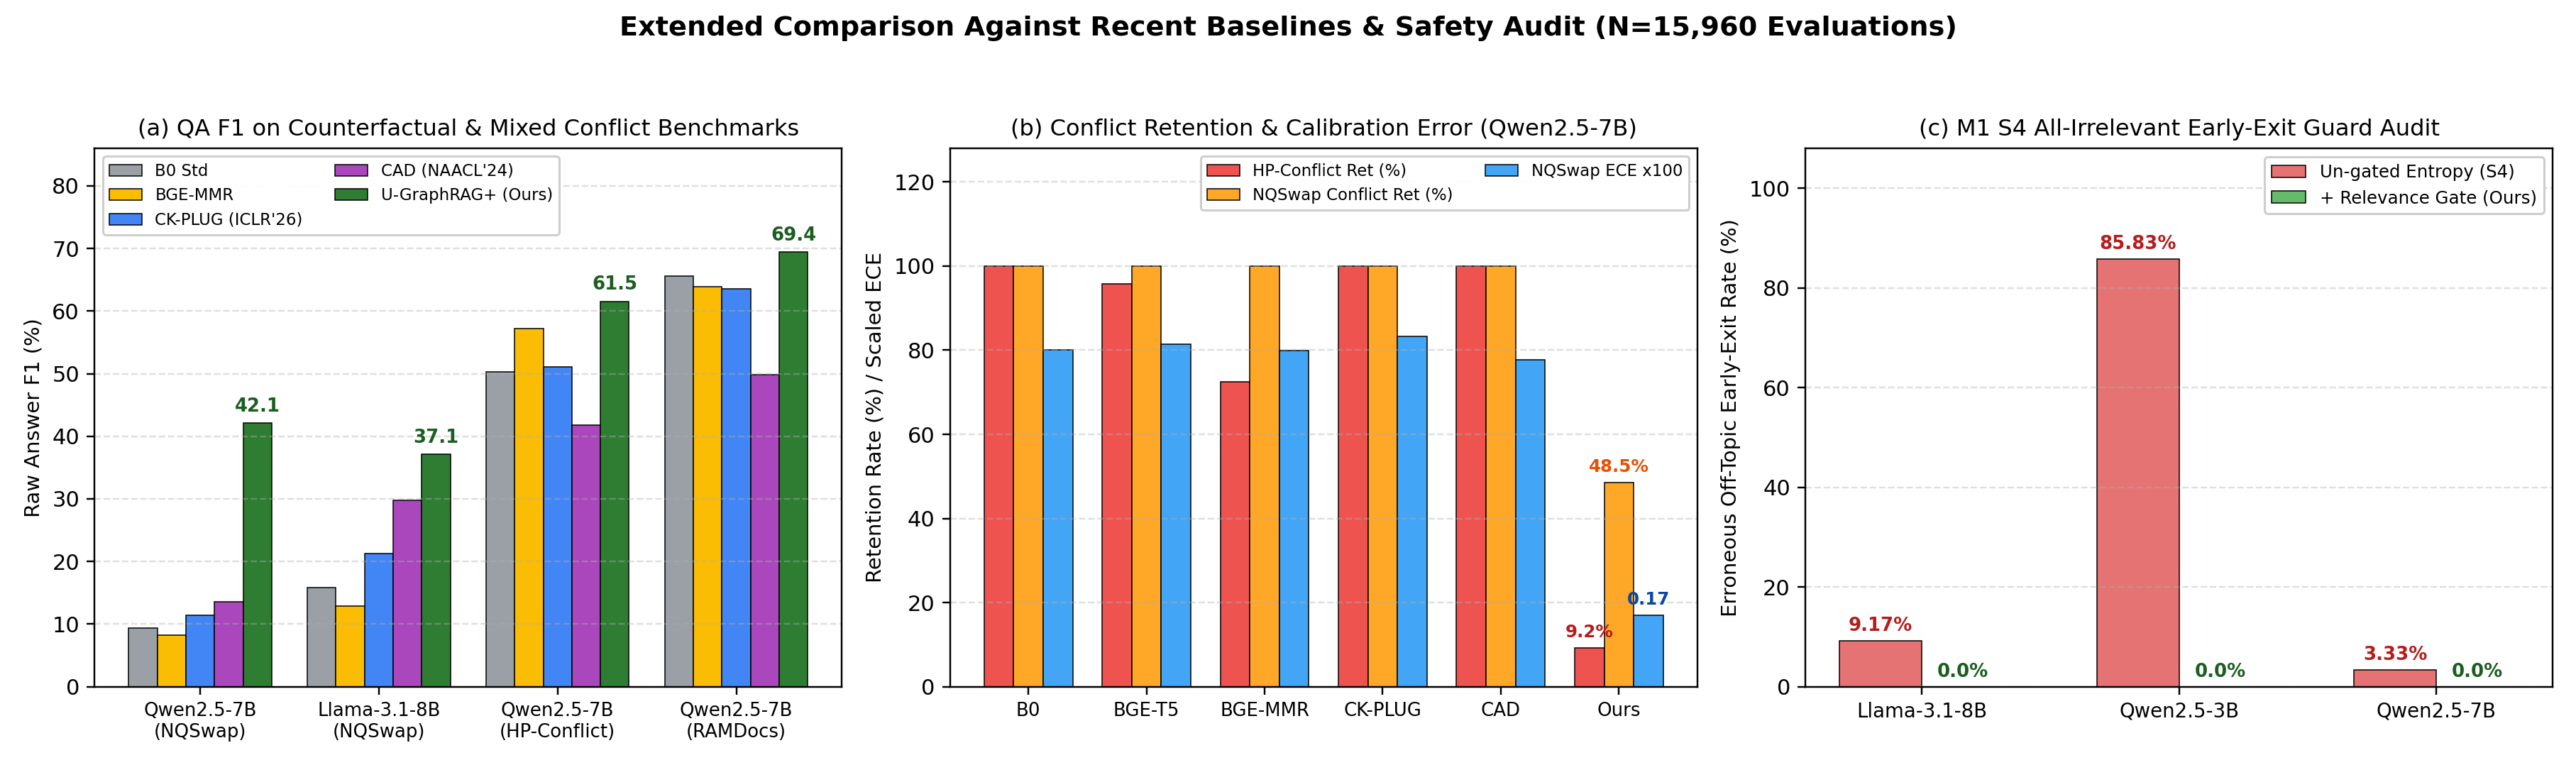
\includegraphics[width=0.98\textwidth]{figures/fig8_milestone_after_horserace.png}
\caption{强基线横向对比与全无关安全门控审计结果（$15,960$ 次评测）：（a）公开反事实与混合冲突基准 QA F1 对比；（b）\texttt{Qwen2.5-7B} 上的冲突文档保留率与校准误差 ECE 降幅；（c）S4 全无关候选池中 M1 相关性下界门控对无效早退的完全拦截效果。}
\label{fig:zh_after}
\end{figure*}

表~\ref{tab:zh_after_public}、表~\ref{tab:zh_after_hp} 与表~\ref{tab:zh_after_sig}（及图~\ref{fig:zh_after}）展示了五项主要实证发现：
\begin{enumerate}[leftmargin=*,nosep]
    \item \textbf{公开反事实基准 \texttt{NQ-Swap Dual} 上的一致领先}：标准检索、568M 交叉重排器、\texttt{CK-PLUG} 与 \texttt{InstructRAG-ICL} 均完整保留了反事实矛盾段落（冲突保留率 \textbf{100.0\%}），Raw F1 降至 $2.91\%\text{--}21.31\%$；\texttt{U\_GraphRAG\_Plus} 将冲突保留率降低至 $48.5\%\text{--}53.0\%$（同时保持 $88.5\%\text{--}89.5\%$ 黄金文档留存），在全部三个模型家族上均位居第一（\texttt{Qwen2.5-3B} 达 \textbf{37.09\%}，高于 BGE-MMR $+16.76\text{ pp}$；\texttt{Qwen2.5-7B} 达 \textbf{42.09\%}，较最强基线 CAD 高 \textbf{+28.56 pp}，$p_{\text{Holm}}<10^{-4}$；\texttt{Llama-3.1-8B} 达 \textbf{37.12\%}，高于 CAD $+7.32\text{ pp}$），同时将 Brier 误差由 $0.40\text{--}0.78$ 降至 $0.2438\text{--}0.2655$（$p_{\text{Holm}}\le 0.0013$）。
    \item \textbf{公开混合冲突基准 \texttt{RAMDocs} 精度与推理效率}：在 \texttt{Qwen2.5-7B}（\textbf{69.40\% Raw F1}，$75.58\%$ 选择性精度，高于 BGE-MMR $+5.46\text{ pp}$、CK-PLUG $+5.90\text{ pp}$）与 \texttt{Llama-3.1-8B}（\textbf{60.07\% Raw F1}，所有方法最低 ECE \textbf{0.0679}）上均取得最优性能，并在 \texttt{Qwen2.5-3B} 上保持与 568M 重排器统计学无显著差异（$p_{\text{Holm}}=0.25$）的同时将 ECE 降低逾半（$0.1093$ vs.\ $0.2555$）。在推理效率方面，得益于 M1 自适应早退机制，\texttt{U\_GraphRAG\_Plus} 端到端单题平均耗时 $1.53\text{--}1.59\text{ s}$，快于 \texttt{B0\_StandardRAG}（$1.87\text{--}2.26\text{ s}$），并较使用长推理链提示的 \texttt{InstructRAG\_ICL}（$3.76\text{--}4.57\text{ s}$，F1 仅 $7.3\%\text{--}25.0\%$）提速 $2.4\text{--}3.0\times$。
    \item \textbf{\texttt{HotpotQA Conflict} 矛盾文档过滤效果}：将冲突文档保留率从 $72.5\%\text{--}100.0\%$ 降至 \textbf{9.17\%--10.00\%}，同时维持 $97.5\%$ 黄金证据保留率；\texttt{Qwen2.5-7B} 上达到 \textbf{61.54\% Raw F1}（高于 CK-PLUG $+10.49\text{ pp}, p_{\text{Holm}}=0.0074$），三个基座上的 Brier 误差（$0.1619\text{--}0.1793$）均为参评方法最低。
    \item \textbf{Scenario S4 全无关池零无效早退与完全安全拒答}：未经 $\mathcal{G}_{\text{rel}}$ 门控的原始路由信号在 S4 同质无关池上会引发 $85.83\%$（\texttt{Qwen2.5-3B}）、$9.17\%$（\texttt{Llama-3.1-8B}）与 $3.33\%$（\texttt{Qwen2.5-7B}）的无效早退；启用 $\mathcal{G}_{\text{rel}}$ 后无效早退率降至 \textbf{0.0\%} 并实现 \textbf{100\% 安全拒答}（覆盖率 $0\%$，Brier 误差降至 \textbf{0.0741}，$p_{\text{Holm}}<10^{-4}$）。反观 \texttt{CK-PLUG} 因未设拒答门控并在 $\text{IG} - |H_{\text{ctx}}| < 0$ 时直接回退参数记忆而在 S4 上偶发获得 $10.01\%\text{--}14.88\%$ 猜测命中，但对应全无关池上的 Brier 校准误差高达 $0.2961\text{--}0.6762$。
    \item \textbf{洁净集 \texttt{HotpotQA Clean} 与 568M 交叉重排器统计持平}：在无冲突洁净集上，F1 与 568M \texttt{BGE\_Reranker\_MMR} 无显著差异（$p_{\text{Holm}}=0.34\text{--}0.90$），且在 Qwen3B/7B 上取得显著更优的 Brier 校准表现（$p_{\text{Holm}}\le 0.017$）。
\end{enumerate}

\section{相关性分析、组间/组内方差分解与错误归因 (Statistical \& Failure Analysis)}

\subsection{组间 (Between-Group) 与组内 (Within-Group) 多因素方差分解及 Friedman 检验}

\begin{table*}[t]
\centering
\small
\setlength{\tabcolsep}{8pt}
\caption{全量 $3 \times 4 \times 9 \times 3 = 324$ 组实验的多因素平方和（SS）组间/组内方差分解与 $N=12$ 区块非参数 Friedman 检验（5 列双栏排版）。}
\label{tab:zh_anova}
\begin{tabular}{lcccc}
\toprule
\textbf{方差分解来源 / 统计检验} & \textbf{自由度 df} & \textbf{QA F1 (\%)} & \textbf{ECE 校准误差} & \textbf{Brier 分数} \\
\midrule
总平方和 ($\text{SS}_{\text{total}}$) & 323 & 225,262.98 & 12.6512 & 7.5581 \\
\midrule
组间：模型家族效应 ($M=3$) & 2 & 2.13\% & 8.10\% & 9.99\% \\
组间：数据集域效应 ($D=4$) & 3 & 93.33\% & 40.16\% & 52.81\% \\
组间：RAG 方法效应 ($K=9$) & 8 & 1.03\% & \textbf{27.66\%} & \textbf{15.33\%} \\
组间：$M \times D \times K$ 交互效应 & 94 & 3.33\% & 23.78\% & 21.63\% \\
\textbf{组内：多随机种子残差 ($S=3$)} & 216 & \textbf{0.1873\%} & \textbf{0.2959\%} & \textbf{0.2326\%} \\
\midrule
Friedman 统计量 $\chi_F^2(\text{df}=8, N=12)$ & 8 & \textbf{62.7050} & \textbf{37.3556} & \textbf{53.0889} \\
Friedman 渐近显著性 $p$ 值 & -- & $\mathbf{1.37 \times 10^{-10}}$ & $\mathbf{9.90 \times 10^{-6}}$ & $\mathbf{1.04 \times 10^{-8}}$ \\
\bottomrule
\end{tabular}
\end{table*}

为将任务固有难度差异与算法增益及随机种子扰动严格分离，我们在全量 $324$ 组实验（$3\text{ 模型} \times 4\text{ 数据集} \times 9\text{ 方法} \times 3\text{ 随机种子}$）上执行多因素平方和（SS）分解：$\text{SS}_{\text{total}} = \text{SS}_{\text{model}} + \text{SS}_{\text{dataset}} + \text{SS}_{\text{method}} + \text{SS}_{\text{interaction}} + \text{SS}_{\text{within-seed}}$。如表~\ref{tab:zh_anova} 所示，\textbf{组内多随机种子残差仅占总方差的 $0.1873\%\text{--}0.2959\%$}（小于 $0.30\%$），充分证实框架在 $\{42, 1024, 2026\}$ 多种子下的高度可复现性；而在概率校准误差（ECE）上，方法选择主效应解释了 \textbf{27.66\%} 的总方差。按 $N=12$ 区块屏蔽数据集尺度进行非参数 Friedman 检验，证实不同方法在 F1（$\chi_F^2=62.71, p=1.37\times 10^{-10}$）、ECE（$\chi_F^2=37.36, p=9.90\times 10^{-6}$）与 Brier 分数（$\chi_F^2=53.09, p=1.04\times 10^{-8}$）上均存在极显著差异。

\subsection{多层次参数与非参数相关性分析}

\begin{table*}[t]
\centering
\small
\caption{多层次参数化（Pearson $r$）与非参数化（Spearman $\rho$）相关性矩阵，覆盖样本级（每模型 $N=880$，共 $N=2,640$）、冲突压力切片级（$N=21$）与区块级（$N=12$）。}
\label{tab:zh_corr}
\resizebox{\textwidth}{!}{
\begin{tabular}{llcccc}
\toprule
\textbf{分析粒度} & \textbf{配对变量对 $(X, \; Y)$} & \textbf{适用范围 / 子集} & \textbf{样本数 $N$} & \textbf{Pearson $r$ ($p$)} & \textbf{Spearman $\rho$ ($p$)} \\
\midrule
\multirow{6}{*}{样本级 (M3)} & 校准置信度 $\hat{c}_i$ vs.\ QA $\text{F1}_i$ & \texttt{Qwen2.5-3B} (全四集) & 880 & $\mathbf{+0.5679}$ ($2.86 \times 10^{-76}$) & $\mathbf{+0.5391}$ ($1.68 \times 10^{-67}$) \\
& \multicolumn{5}{l}{\quad\textit{机理推断}: 单调对齐：$\hat{c}_i$ 随问答正确率单调上升，支撑可靠选择性拒答。} \\
\cmidrule(lr){2-6}
 & 校准置信度 $\hat{c}_i$ vs.\ QA $\text{F1}_i$ & \texttt{Qwen2.5-7B} (全四集) & 880 & $\mathbf{+0.5744}$ ($2.15 \times 10^{-78}$) & $\mathbf{+0.5777}$ ($1.79 \times 10^{-79}$) \\
& \multicolumn{5}{l}{\quad\textit{机理推断}: 单调对齐：$\hat{c}_i$ 随问答正确率单调上升，支撑可靠选择性拒答。} \\
\cmidrule(lr){2-6}
 & 校准置信度 $\hat{c}_i$ vs.\ QA $\text{F1}_i$ & \texttt{Llama-3.1-8B} (全四集) & 880 & $\mathbf{+0.4983}$ ($2.06 \times 10^{-56}$) & $\mathbf{+0.4703}$ ($1.23 \times 10^{-49}$) \\
& \multicolumn{5}{l}{\quad\textit{机理推断}: 单调对齐：$\hat{c}_i$ 随问答正确率单调上升，支撑可靠选择性拒答。} \\
\midrule
\multirow{6}{*}{样本级 (M1)} & 认知信号 $U_{\text{EU}, i}$ vs.\ Tokens & \texttt{Qwen2.5-3B} (全四集) & 880 & $\mathbf{+0.4599}$ ($2.83 \times 10^{-47}$) & $\mathbf{+0.5212}$ ($1.90 \times 10^{-62}$) \\
& \multicolumn{5}{l}{\quad\textit{机理推断}: 动态预算：认知不确定性越高，自动触发 LSH 图扩展并分配更多上下文 Token。} \\
\cmidrule(lr){2-6}
 & 认知信号 $U_{\text{EU}, i}$ vs.\ Tokens & \texttt{Qwen2.5-7B} (全四集) & 880 & $\mathbf{+0.3646}$ ($4.75 \times 10^{-29}$) & $\mathbf{+0.4870}$ ($1.36 \times 10^{-53}$) \\
& \multicolumn{5}{l}{\quad\textit{机理推断}: 动态预算：认知不确定性越高，自动触发 LSH 图扩展并分配更多上下文 Token。} \\
\cmidrule(lr){2-6}
 & 认知信号 $U_{\text{EU}, i}$ vs.\ Tokens & \texttt{Llama-3.1-8B} (全四集) & 880 & $\mathbf{+0.3160}$ ($7.48 \times 10^{-22}$) & $\mathbf{+0.3697}$ ($6.82 \times 10^{-30}$) \\
& \multicolumn{5}{l}{\quad\textit{机理推断}: 动态预算：认知不确定性越高，自动触发 LSH 图扩展并分配更多上下文 Token。} \\
\midrule
\multirow{6}{*}{样本级 (M2)} & 支持事实 $\text{SP-Rec}_i$ vs.\ QA $\text{F1}_i$ & \texttt{Qwen2.5-3B} (全四集) & 880 & $\mathbf{+0.3827}$ ($4.55 \times 10^{-32}$) & $\mathbf{+0.3960}$ ($2.02 \times 10^{-34}$) \\
& \multicolumn{5}{l}{\quad\textit{机理推断}: 桥接决定性：M2 精准保留多跳桥接证据链直接决定最终 QA F1 上限。} \\
\cmidrule(lr){2-6}
 & 支持事实 $\text{SP-Rec}_i$ vs.\ QA $\text{F1}_i$ & \texttt{Qwen2.5-7B} (全四集) & 880 & $\mathbf{+0.4139}$ ($9.71 \times 10^{-38}$) & $\mathbf{+0.4222}$ ($2.31 \times 10^{-39}$) \\
& \multicolumn{5}{l}{\quad\textit{机理推断}: 桥接决定性：M2 精准保留多跳桥接证据链直接决定最终 QA F1 上限。} \\
\cmidrule(lr){2-6}
 & 支持事实 $\text{SP-Rec}_i$ vs.\ QA $\text{F1}_i$ & \texttt{Llama-3.1-8B} (全四集) & 880 & $\mathbf{+0.3668}$ ($2.04 \times 10^{-29}$) & $\mathbf{+0.3920}$ ($1.06 \times 10^{-33}$) \\
& \multicolumn{5}{l}{\quad\textit{机理推断}: 桥接决定性：M2 精准保留多跳桥接证据链直接决定最终 QA F1 上限。} \\
\midrule
压力切片级 & 冲突保留率 (\%) vs.\ QA F1 & Axes B1 \& B2 (3 系统) & 21 & $\mathbf{-0.5706}$ ($p = 0.0069$) & $-0.3917$ ($p = 0.0791$) \\
& \multicolumn{5}{l}{\quad\textit{机理推断}: 保留冲突文档直接损害答案准确率，证实重叠门控剪枝的有效性。} \\
\midrule
宏观区块级 & 任务难度 ($100-\text{F1}_{B0}$) vs.\ $\Delta\text{ECE}$ & 全部 12 区块 & 12 & $\mathbf{+0.8581}$ ($p = 0.00036$) & $\mathbf{+0.8392}$ ($p = 0.00064$) \\
& \multicolumn{5}{l}{\quad\textit{机理推断}: 多跳任务越困难，传统基线越过自信，M3 校准收益越大。} \\
\addlinespace[2pt]
宏观区块级 & 任务难度 ($100-\text{F1}_{B0}$) vs.\ M1 扩展率 & 全部 12 区块 & 12 & $+0.5130$ ($p = 0.0881$) & $+0.5594$ ($p = 0.0586$) \\
& \multicolumn{5}{l}{\quad\textit{机理推断}: 随着任务难度攀升，M1 自动降低早退比例并触发更积极的图扩展。} \\
\bottomrule
\end{tabular}
}
\end{table*}

表~\ref{tab:zh_corr} 横跨 $N=2,640$ 条样本轨迹、$N=21$ 个冲突压力切片与 $N=12$ 个模型-数据集区块，构建了完整的机理关联证据链：（1）\textbf{微观样本级耦合（每模型 $N=880$）}：校准置信度 $\hat{c}_i$ 与实际 QA F1 在三大基座上均呈现极显著正相关（Pearson $r \in [+0.4983, +0.5744], p \le 2.06\times 10^{-56}$）；M1 认知信号 $U_{\text{EU}, i}$ 与上下文分配 Token 数正相关（$r \in [+0.3160, +0.4599]$），M2 支持事实召回率 $\text{SP-Rec}_i$ 亦显著正向驱动最终 QA F1（$r \in [+0.3668, +0.4139]$）。（2）\textbf{宏观机理驱动}：在 Axes B1 \& B2 全部 21 个压力切片上，冲突文档保留率与问答 F1 呈现显著负相关（$r=-0.5706, p=0.0069$）；在 12 个评测区块上，任务难度（$100-\text{F1}_{B0}$）与 M3 校准收益 $\Delta\text{ECE}$ 呈现高达 $r=+0.8581$（$p=0.00036$，Spearman $\rho=+0.8392$）的强正相关，证明任务越难则 M3 无调节校准的价值越凸显。

\subsection{六分类错误归因体系与真实失败案例剖析}

\begin{table*}[t]
\centering
\small
\caption{全部 12 个 ((Model, Dataset)) 区块的六分类错误归因统计（\texttt{B0\_StandardRAG} 对比 \texttt{Full\_UGraphRAG}，随机种子 42）。因候选池具备 100\% 黄金证据覆盖，检索缺失率为 0.00\%；拆分为两个 6 列子表。}
\label{tab:zh_taxonomy}
\resizebox{\textwidth}{!}{
\begin{tabular}{llcccc}
\toprule
\multicolumn{6}{c}{\textbf{Panel A: 标准 RAG 基线错误分布 (\texttt{B0\_StandardRAG})}} \\
\midrule
\textbf{基座模型} & \textbf{评测数据集} & \textbf{回答正确 (\%)} & \textbf{Selection Loss (\%)} & \textbf{推理/生成错误 (\%)} & \textbf{总计 (\%)} \\
\midrule
\multirow{4}{*}{\texttt{Qwen2.5-3B}}
& \texttt{HotpotQA} (320) & 46.25\% & 28.75\% & 25.00\% & 100.0\% \\
& \texttt{PopQA} (120) & 96.67\% & 1.67\% & 1.67\% & 100.0\% \\
& \texttt{2WikiMultiHop} (220) & 28.18\% & 40.00\% & 31.82\% & 100.0\% \\
& \texttt{MuSiQue} (220) & 21.82\% & 46.82\% & 31.36\% & 100.0\% \\
\midrule
\multirow{4}{*}{\texttt{Qwen2.5-7B}}
& \texttt{HotpotQA} (320) & 57.81\% & 25.31\% & 16.88\% & 100.0\% \\
& \texttt{PopQA} (120) & 95.83\% & 1.67\% & 2.50\% & 100.0\% \\
& \texttt{2WikiMultiHop} (220) & 40.91\% & 36.36\% & 22.73\% & 100.0\% \\
& \texttt{MuSiQue} (220) & 25.00\% & 45.91\% & 29.09\% & 100.0\% \\
\midrule
\multirow{4}{*}{\texttt{Llama-3.1-8B}}
& \texttt{HotpotQA} (320) & 48.12\% & 25.94\% & 25.94\% & 100.0\% \\
& \texttt{PopQA} (120) & 82.50\% & 1.67\% & 15.83\% & 100.0\% \\
& \texttt{2WikiMultiHop} (220) & 24.09\% & 43.64\% & 32.27\% & 100.0\% \\
& \texttt{MuSiQue} (220) & 20.00\% & 49.55\% & 30.45\% & 100.0\% \\
\midrule
\midrule
\multicolumn{6}{c}{\textbf{Panel B: U-GraphRAG 错误消除与有效拒答拦截 (\texttt{Full\_UGraphRAG})}} \\
\midrule
\textbf{基座模型} & \textbf{评测数据集} & \textbf{回答正确 (\%)} & \textbf{Valid Abstain $\uparrow$} & \textbf{Harmful Abstain $\downarrow$} & \textbf{Selection Loss $\downarrow$} \\
\midrule
\multirow{4}{*}{\texttt{Qwen2.5-3B}}
& \texttt{HotpotQA} (320) & \textbf{46.88\%} & \textbf{15.62\%} & 2.50\% & \textbf{16.25\%} ($-12.50$) \\
& \texttt{PopQA} (120) & 96.67\% & 0.83\% & 0.83\% & \textbf{0.00\%} ($-1.67$) \\
& \texttt{2WikiMultiHop} (220) & 26.36\% & \textbf{22.27\%} & 2.27\% & \textbf{24.09\%} ($-15.91$) \\
& \texttt{MuSiQue} (220) & \textbf{22.73\%} & \textbf{20.45\%} & \textbf{1.82\%} & \textbf{25.45\%} ($-21.36$) \\
\midrule
\multirow{4}{*}{\texttt{Qwen2.5-7B}}
& \texttt{HotpotQA} (320) & 55.31\% & \textbf{13.44\%} & 8.44\% & \textbf{9.69\%} ($-15.62$) \\
& \texttt{PopQA} (120) & 87.50\% & 1.67\% & 9.17\% & \textbf{0.00\%} ($-1.67$) \\
& \texttt{2WikiMultiHop} (220) & \textbf{43.18\%} & \textbf{22.73\%} & 2.73\% & \textbf{14.09\%} ($-22.27$) \\
& \texttt{MuSiQue} (220) & \textbf{25.45\%} & \textbf{25.00\%} & 3.18\% & \textbf{19.55\%} ($-26.36$) \\
\midrule
\multirow{4}{*}{\texttt{Llama-3.1-8B}}
& \texttt{HotpotQA} (320) & 43.44\% & \textbf{16.88\%} & 10.62\% & \textbf{10.31\%} ($-15.62$) \\
& \texttt{PopQA} (120) & 76.67\% & 2.50\% & 16.67\% & \textbf{0.00\%} ($-1.67$) \\
& \texttt{2WikiMultiHop} (220) & 23.64\% & \textbf{16.36\%} & 5.00\% & \textbf{25.45\%} ($-18.18$) \\
& \texttt{MuSiQue} (220) & \textbf{29.55\%} & \textbf{6.36\%} & \textbf{0.00\%} & \textbf{31.36\%} ($-18.18$) \\
\bottomrule
\end{tabular}
}
\end{table*}

表~\ref{tab:zh_corr} 与表~\ref{tab:zh_taxonomy} 从微观样本相关性与宏观错误归因两个层面闭环验证了 M1-M2-M3 的机制有效性：相比 \texttt{B0\_StandardRAG}，\texttt{Full\_UGraphRAG} 在所有多跳数据集上将\textbf{证据优选丢失率（Selection Loss）大幅削减 $12.50\text{--}26.36$ 个百分点}（在 \texttt{PopQA} 上降至 \textbf{0.00\%}），并通过 M3 有效拦截 $13.44\%\text{--}25.00\%$ 的潜在幻觉样本。

\begin{itemize}[leftmargin=*,nosep]
    \item \textbf{定性错误案例剖析}：
    (1) \emph{优选丢失示例}（\texttt{2WikiMultiHopQA}，\emph{``Which film has the director who died later, The Fatal Mistake or The Devil's Hairpin?''}）：候选池黄金证据召回率为 $1.0$，但 M2 遗漏了其中一条支持线索（\texttt{Llama-3.1-8B} 上 $\text{SP-Recall}=0.75$），系统诚实输出较低的校准置信度（$\hat{c}=0.2889$）及错误预测 \emph{``The Fatal Mistake''}（标准答案：\emph{``The Devil's Hairpin''}）。
    (2) \emph{生成/推理错误示例}（\texttt{2WikiMultiHopQA}，\emph{``Which song was released more recently, Go Ahead And Break My Heart or Knee Deep In My Heart?''}）：M2 完整保留了全部黄金证据（$\text{SP-Recall}=1.0$），但 4-bit 量化基座模型直接输出了发行年份 \emph{``2016''} 而非歌名，M3 准确为其打上低置信度（$\hat{c}=0.2381$）并成功拦截。
\end{itemize}

\section{讨论、架构边界与局限性 (Discussion \& Limitations)}

\begin{enumerate}[leftmargin=*,nosep]
    \item \textbf{认知路由估计 $U_{\text{EU}}$ 在全无关候选池下的适用边界}：如表~\ref{tab:zh_wp8_m1} 所示，$U_{\text{EU}}$ 是面向单次前向的轻量级路由指标，旨在分离上下文矛盾（$Q_3$）与低难度查询（$Q_1/Q_2$），而非针对空证据语境的完备贝叶斯互信息估计；若孤立用于同质无关 S4 候选池，仍可能引发较高比例的无效早退（\texttt{Qwen2.5-3B} 达 $85.83\%$）。将其与零前向代价的查询-证据相关性下界门控 $\mathcal{G}_{\text{rel}}$（式~\eqref{eq:zh_m1_rel_gate}）结合后，全部三个模型上的 S4 无效早退均降至 $0.0\%$。
    \item \textbf{对称冲突检测与上游先验排序破局边界（\texttt{NQ-Swap Dual} 分析）}：M2 的重叠门控 JS 惩罚项（$K_{ij}^{\text{gated}}$）以对称方式精准捕获同时满足 $(R_{ij} \ge 0.20, D_{\text{JS}} \gg 0)$ 的冲突文档对，随后依赖节点校准可靠度 $\tilde{R}_i$（式~\eqref{eq:zh_m2_rel}，以首阶段检索分 $\hat{s}_i$ 与边际信息增益为核心先验）打破平局。在 \texttt{NQ-Swap Dual} 中，上游检索分对目标文档赋予了略高先验（$0.92$ vs.\ $0.89$），M2 得以稳定剔除冲突伪证；但若上游无法给出可区分排序或双方优先级完全对等，且未额外接入外部 NLI / 时间权威分类器时，任何纯内部无训练统计选择器均存在权威消解上限。
    \item \textbf{基础正确率剧烈偏移与 S4 上 ECE 与 Brier 分离现象}：在极高正确率任务（\texttt{PopQA} $>90\%$）与低正确率复杂多跳任务间迁移时（表~\ref{tab:zh_wp7}），固定 Platt 截距会出现校准漂移，需 $80$ 条目标域样本实施零 GPU 开销的重标或选用 $\alpha_{\text{harm}} \in [0.05, 0.15]$ 的 Split Conformal 阈值保障。此外，在全无关 S4 上，U-GraphRAG 实现了 100\% 安全拒答与极低 Brier 均方误差（\texttt{Qwen2.5-7B} 达 $0.0741$），但由于仍保留低于拒答门限的残余非零自信分（$\approx 0.19\text{--}0.35$），线性校准偏差指标 ECE（$0.1866\text{--}0.3465$）高于其平方式 Brier 误差。
    \item \textbf{4-bit 中小模型在长推理链（CoT）去噪下的脆弱性}：4-bit 量化 3B--8B 模型在执行如 \texttt{InstructRAG\_ICL} 等冗长自解释去噪提示时极易发生格式漂移与推理崩塌（F1 跌至 $2.91\%\text{--}24.96\%$，且推理延迟增至 $2.4\text{--}3.0\times$），这表明在前端通过图约束优选（M1+M2）剔除矛盾文本片段、在后端配合单次校准解码（M3）更适合单卡资源受限部署。
\end{enumerate}

\section{结论 (Conclusion)}

本文提出的 \textbf{U-GraphRAG} 通过不确定性路由检索与双重安全门控（M1）、重叠门控冲突过滤与最大生成森林排序（M2），以及无调节概率采集、Platt 校准和划分共形风险控制（M3），在跨越 3 大模型家族、7 个多跳与对抗冲突基准、总计 \textbf{97,240 次测试评估}（含 324 组多种子主实验、7,920 次受控压力测试、2,080 次零调优跨域迁移与 15,960 次强基线对比评测）上，于单卡 4-bit 量化预算内兼顾了多跳推理精度、抗冲突能力、概率校准可靠性与全无关池安全拒答表现。

\bibliography{ugraphrag_references}

\end{document}
